%\documentclass[journal=jpcbfk,manuscript=article]{achemso}
\documentclass{article}

\usepackage{graphicx}
\usepackage{wrapfig}
\usepackage{subcaption}
\usepackage{amsmath} 
\usepackage[margin=1in]{geometry}\usepackage{amsmath} % or simply amstext
\usepackage{siunitx}
\usepackage{booktabs}
\usepackage[export]{adjustbox}
\newcommand{\angstrom}{\textup{\AA}}
\usepackage{cleveref}
\usepackage{booktabs}
\usepackage{gensymb}
\usepackage{float}
\usepackage{listings}
\usepackage{xr}
\usepackage{array}
\newcolumntype{P}[1]{>{\centering\arraybackslash}p{#1}}

\renewcommand{\thefigure}{S\arabic{figure}}
\renewcommand{\thesection}{S\arabic{section}}   

%\SectionNumbersOn

\externaldocument[M-]{Final_Draft}
\title{Supporting Information : Understanding the Nanoscale Structure of Inverted Hexagonal Phase Lyotropic Liquid Crystal Polymer Membranes}
\author{Benjamin J. Coscia \and Jospeh Yelk \and Matthew A. Glaser \and Douglas L. Gin \and Xunda Feng \and Michael R. Shirts}
\date{}

\begin{document}

  \bibliographystyle{ieeetr}
  \graphicspath{{./figures/}}  % put all the figures here
  \maketitle
  
  \section{Setup and analysis scripts}\label{section:python_scripts}
  
  All python and bash scripts used to set up systems and conduct post-simulation trajectory
  analysis, except for simulating X-ray diffraction (XRD) patterns, are available online at
  \texttt{https://github.com/bencoscia/llcsim}. Table~\ref{table:python_scripts} provides more 
  detail about specific scripts used for each type of analysis performed in the main text.
  
  The python scripts used to simulated XRD patterns are publicly available online at \\
  \texttt{https://github.com/joeyelk/MD-Structure-Factor}. Given a GROMACS trajectory 
  (.trr or .xtc) and a configuration file (.gro), simulate an XRD pattern using
  \texttt{main\_gromacs.py}. Pass the flag \texttt{\--manuscript\_format} to generate patterns
  and cross-sections with the same format as those presented in the main text.

  \section{Further details regarding monomer parameterization}\label{section:parameterization}
 
  We parameterized monomers according to the following procedure:
  \begin{enumerate}
  
	\item \textit{Create monomer structure file with connectivity}: We
	drew atomistic structures using MarvinSketch
	17.13~\cite{chemaxon_marvinsketch_2017} with all hydrogen atoms drawn out
	explicitly. We optimized the 3D geometry of the structure using the `Clean in
	3D' function of MarvinSketch.  We saved the structure as a .mol file, then
	converted it to .pdb format using Open Babel 2.4.1
	\cite{oboyle_open_2011,noauthor_open_nodate}. 
	
	\item \textit{Assign GAFF atomtypes using \texttt{antechamber}}: Using
	the .pdb structure file as input, we ran
	\texttt{antechamber}~\cite{wang_automatic_2006} using the AM1-BCC charge model.
	The net charge on the monomer is input as -1 since the sodium ion is kept as 
	a separate residue. We use \texttt{LEaP}~\cite{case_ambertools16_2016} and the
	output of \texttt{antechamber} to create Amber topology files. A detailed
	tutorial for using \texttt{LEaP} for parameterization can be accessed elsewhere \cite{walker_antechamber_nodate}.

	\item \textit{Create GROMACS topologies from Amber output}: The output
	of \texttt{LEaP} is a .inpcrd and a .prmtop file which are Amber topology
	files. Using acpype.py \cite{sousa_da_silva_acpype_2012}, we converted the
	\texttt{LEaP} output into GROMACS .gro and .top files. 

	\item \textit{Perform a simulated annealing procedure on the monomer}:
	We created a cubic box around the monomer using the GROMACS command \texttt{gmx
	editconf}. The monomer was centered in the box with edges of the
	box spaced at least 3 nm from the monomer on all sides. We ran an energy minimization
	on the system with the steepest descent algorithm. Next we performed an NVT
	simulated annealing procedure. We linearly decreased the temperature of the
	system from 1000 K to 50 K over the course of 10 ns. We randomly chose a monomer
	configuration from the last 10\% of the trajectory. 

	\item \textit{Reassign charges with \texttt{molcharge}}: With the monomer
	configuration taken from the annealed trajectory, we reassigned charges using
	\texttt{molcharge} with the am1bccsym method in order to ensure charges 
	are symmetric. This condition is not guaranteed with \texttt{antechamber}. 
	The charges in the GROMACS topology file (.top) were replaced with the 
	new charges calculated by \texttt{molcharge}. 

	\item \textit{Anneal again to get final structure}: We repeated the
	same simulated annealing procedure using the monomer topology with
	\texttt{molcharge} charges. A random monomer configuration was pulled from the
	last 10\% of the trajectory and was used to build all assemblies reported
	(Figure~\ref{fig:monomer}).
	
  \end{enumerate} 

  \begin{figure}[!htb]
	\centering
        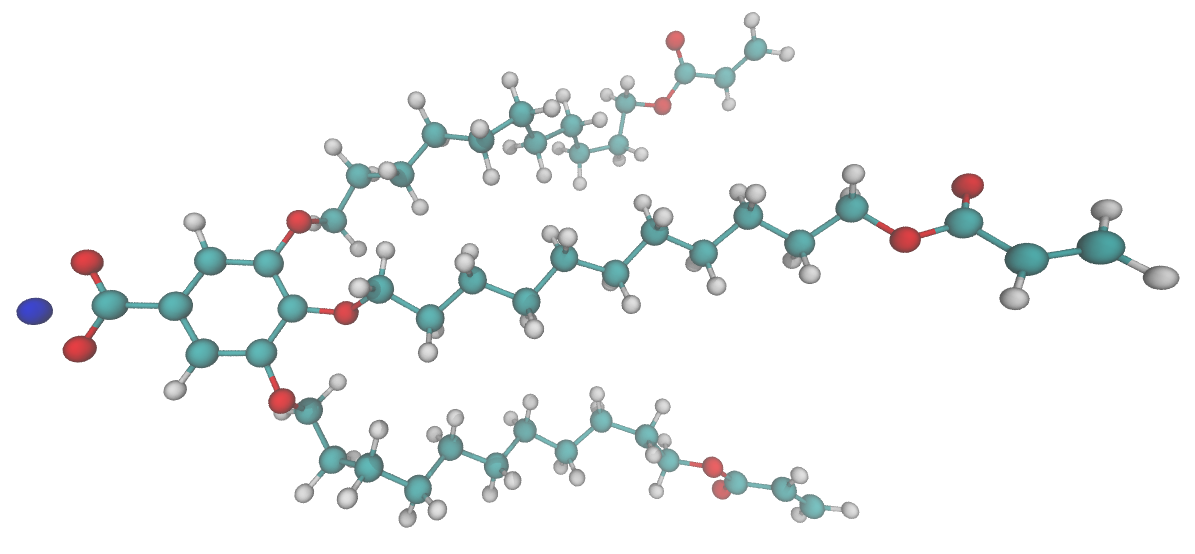
\includegraphics[width=0.9\textwidth]{monomer.png}
	\caption{Atomistic representation of the monomer Na-GA3C11. White atoms
		represent hydrogen, cyan atoms represent carbon, red atoms represent oxygen and
		the blue atom is sodium.}\label{fig:monomer}
  \end{figure}
  
  \clearpage

  \begin{table}[htb!]
  \centering
  \newcolumntype{A}{ >{\centering\arraybackslash} m{2.25in} }
  \newcolumntype{B}{ >{\centering\arraybackslash} m{0.75in} }
  \newcolumntype{C}{m{3in}}
  \begin{tabular}{|A|B|C|}
  \hline
  \textbf{Script Name} & \textbf{Section} & ~~~~~~~~~~~~~~~~~~~~~\textbf{Description} \\
  \hline
  \texttt{/setup/param.sh} & \ref{M-method:parameterization} & Automatically run the monomer
  parameterization scheme outlined in Section~\ref{section:parameterization} given an initial
  structure file in .pdb format. \\ \hline
  
  \texttt{/setup/build.py} & \ref{M-method:unitcell_build} \& \ref{M-method:monomer_placement} &
  Build an initial configuration in the sandwiched or parallel displaced configuration with the 
  desired initial vertical monomer spacing, monomers-per-column, and columns-per-pore. \\ \hline
  
  \texttt{/setup/equil.sh} & \ref{M-section:equilibration} & Wrapper script for running the GROMACS 
  functions and python scripts needed in order to equilibrate an initial configuration. \\ \hline
   
  \texttt{/analysis/Structure\_char.py} & \ref{M-method:pore_spacing} & Calculate the distance 
  between pores. \\ \hline
  
  \texttt{/analysis/correlation.py} & \ref{M-section:correlation_length} & Calculate the 3D 
  correlation function from a trajectory and plot desired slices. \\ \hline
  
  \texttt{/analysis/regional\_density.py} & \ref{M-method:rdfs} & Calculate the density of a given
  monomer component as a function of its distance from the pore center. \\ \hline
  
  \texttt{/analysis/structure\_factor.py} & \ref{M-method:simple_systems} & Generate customizable
  trajectories of point scatterers, then calculate their structure factor and plot slices of it.
  \\ \hline 
  
  \texttt{/analysis/disorder.py} & \ref{M-method:simple_systems} & Measure the magnitude of
  quenched disorder. \\ \hline
  
  \texttt{/analysis/Ionic\_Conductivity.py} & \ref{M-method:ionic_conductivity} & Calculate the 
  ionic conductivity using the Nernst-Einsten relationship and collective diffusion model. \\ \hline
  
  \texttt{/setup/xlink.py} & \ref{M-method:xlink} & Iteratively cross-link a system given an 
  initial configuration. \\ \hline
    
  \texttt{/analysis/orientational\_order.py} & \ref{M-section:mon_per_pore} & Calculate the 
  nematic order parameter. \\ \hline
  
  \texttt{/analysis/tilt.py} & \ref{M-section:rspots} & Calculate the angle between the xy plane
  and the vector extending from the front to the back of each monomer tail. \\ \hline
  
  \texttt{/analysis/tail\_packing.py} & \ref{M-section:rspots} & Calculate the distribution of
  angles between the center of mass of each monomer tail and its nearest neighbor monomer tails.
  \\ \hline
 
  \texttt{/analysis/compare\_disorder.py} & \ref{M-section:rpi} & Measure quenched disorder for
  each trajectory in an ensemble of simulations, then plot distributions of quenched disorder.
  \\ \hline
  
  \texttt{/analysis/hbonds\_pairing.py} & \ref{M-section:rdouble} & Identify all hydrogen bonds
  then count the number of monomer pairs that share hydrogen bonds. \\ \hline
  
  \texttt{/analysis/torsions.py} & \ref{M-section:slow_dynamics} & Calculate the autocorrelation
  function for a chosen dihedral. \\ \hline
  
  \end{tabular}
  
  \caption{The first column provides the names of the python scripts available in
  the \texttt{llcsim} GitHub repository that were used for system setup and post-simulation 
  trajectory analysis. Paths preceding script names are relative to the 
  \texttt{llcsim} root directory. The second columns lists the section in the main
  text where the output or usage of the script is first described. The third column
  gives a brief description of the purpose of each script.
  }~\label{table:python_scripts}
  
  \end{table}
  
  \clearpage
  
  \section{Attempted Self-assembly}\label{section:self_assembly}
  
  We attempted self assembly of Na-GA3C11 monomers by using an isotropic configuration
  generated using Packmol \cite{martinez_packmol:_2009} (Figure~\ref{fig:isotropic_box}).
  The input file given to Packmol is shown below.
  
  \lstset{language=bash}
  \begin{lstlisting}
  tolerance 2.0
  output packed.pdb
  filetype pdb
  structure monomer.pdb
  		number 400
  		inside box 0. 0. 0. 84.3 84.3 84.3
  end structure
  \end{lstlisting}

  We used the same number of monomers (400) that we used in all other simulations. 
  Since Packmol does not have the capability to create monoclinic boxes, we used a cubic
  box with a volume of 660 nm$^3$, 25\% larger than those used to create ordered unit
  cells we studied. We tested systems with semi-isotropic and anisotropic pressure 
  coupling since the shape of the unit cell will likely need to change in order to 
  accommodate hexagonally packed pores.
  
  We use the nematic order parameter as defined in Section~\ref{method:nematic_order} to 
  observe any progress towards system ordering. In both cases, we see that the nematic
  order parameter stays close to zero for the duration of the simulation time, indicating
  an isotropic arrangement of head groups (Figure~\ref{fig:nematic_isotropic}). The values
  are slightly negative since there are only 400 monomers. 
  Equation~\ref{eqn:nematic_order_parameter} is bounded between -1 and 1, however, with a
  proper choice of nematic director, measured values will range between 0 and 1. With a 
  large number of samples, an isotropic system would have an order parameter of 0.
  
  \begin{figure}[!htb]
  \centering
  \begin{subfigure}{0.45\textwidth}
  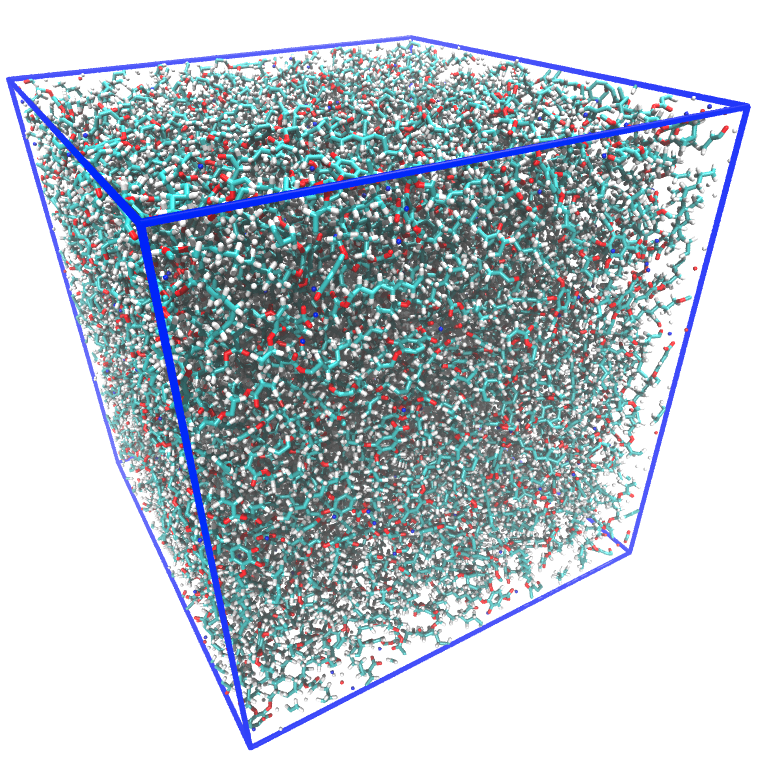
\includegraphics[width=\textwidth]{isotropic_box.png}
  \caption{}\label{fig:isotropic_box}
  \end{subfigure}
  \begin{subfigure}{0.45\textwidth}
  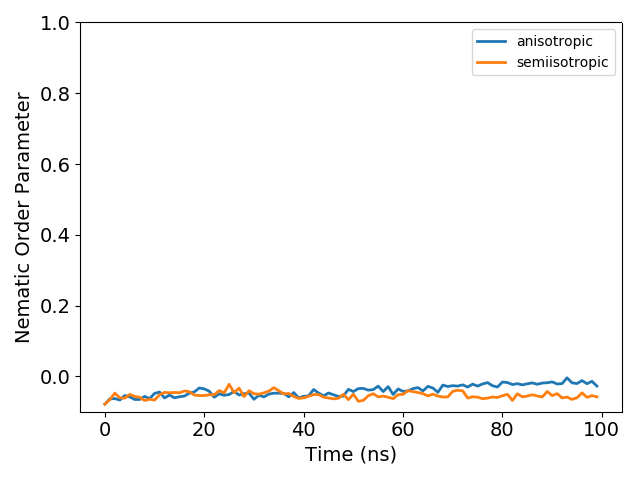
\includegraphics[width=\textwidth]{nematic_isotropic.png}
  \caption{}\label{fig:nematic_isotropic}
  \end{subfigure}
  \caption{(a) We created a box of isotropically packed monomers and allowed it to simulate
  for 100 ns using isotropic and anisotropic pressure coupling. (b) The nematic order 
  parameter hovers close to zero for the duration of the simulation meaning the system
  maintains its isotropic alignment.}\label{fig:self_assembly}
  \end{figure}
  
  \clearpage  
  
  \section{Monomer build procedure}\label{section:monomer_build_procedure}
  
  Figure~\ref{fig:build_procedure} illustrates the procedure carried out by 
  \texttt{build.py} in order to build initial configurations.  
  
  \begin{figure}[!htb]
  \centering
  \begin{subfigure}[t]{0.45\textwidth}
  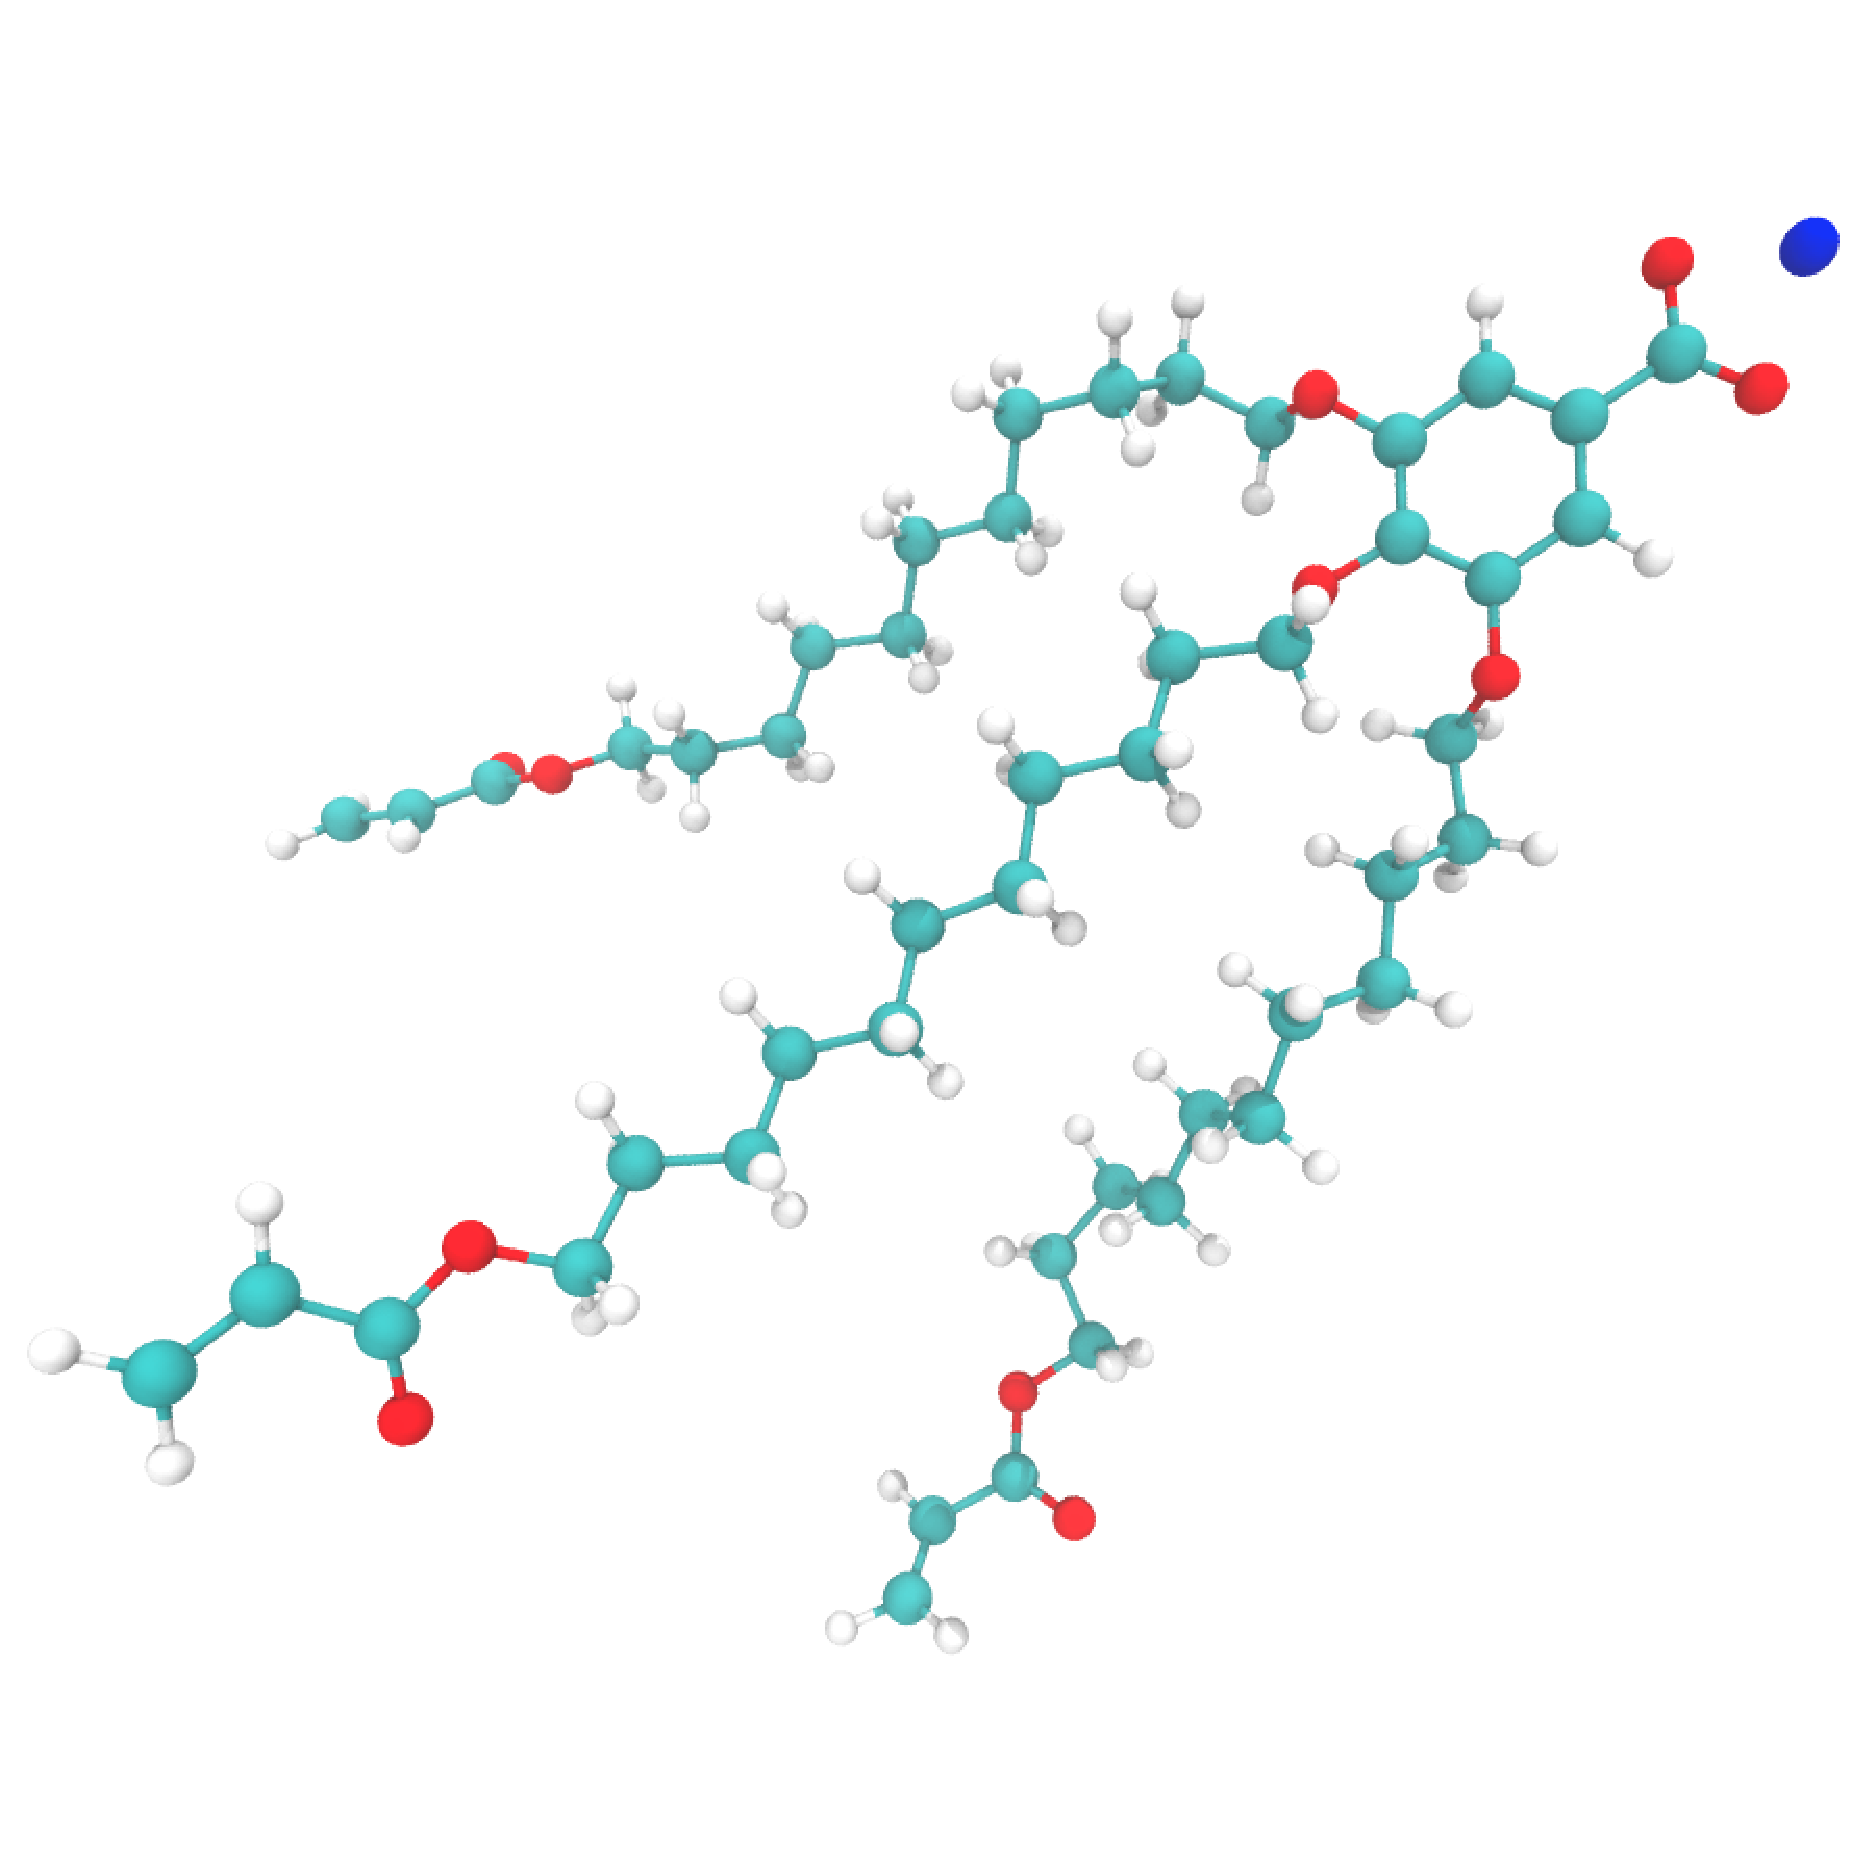
\includegraphics[width=\linewidth]{monomer_diagonal.pdf}
  \caption{}
  \end{subfigure}
  \begin{subfigure}[t]{0.42\textwidth}
  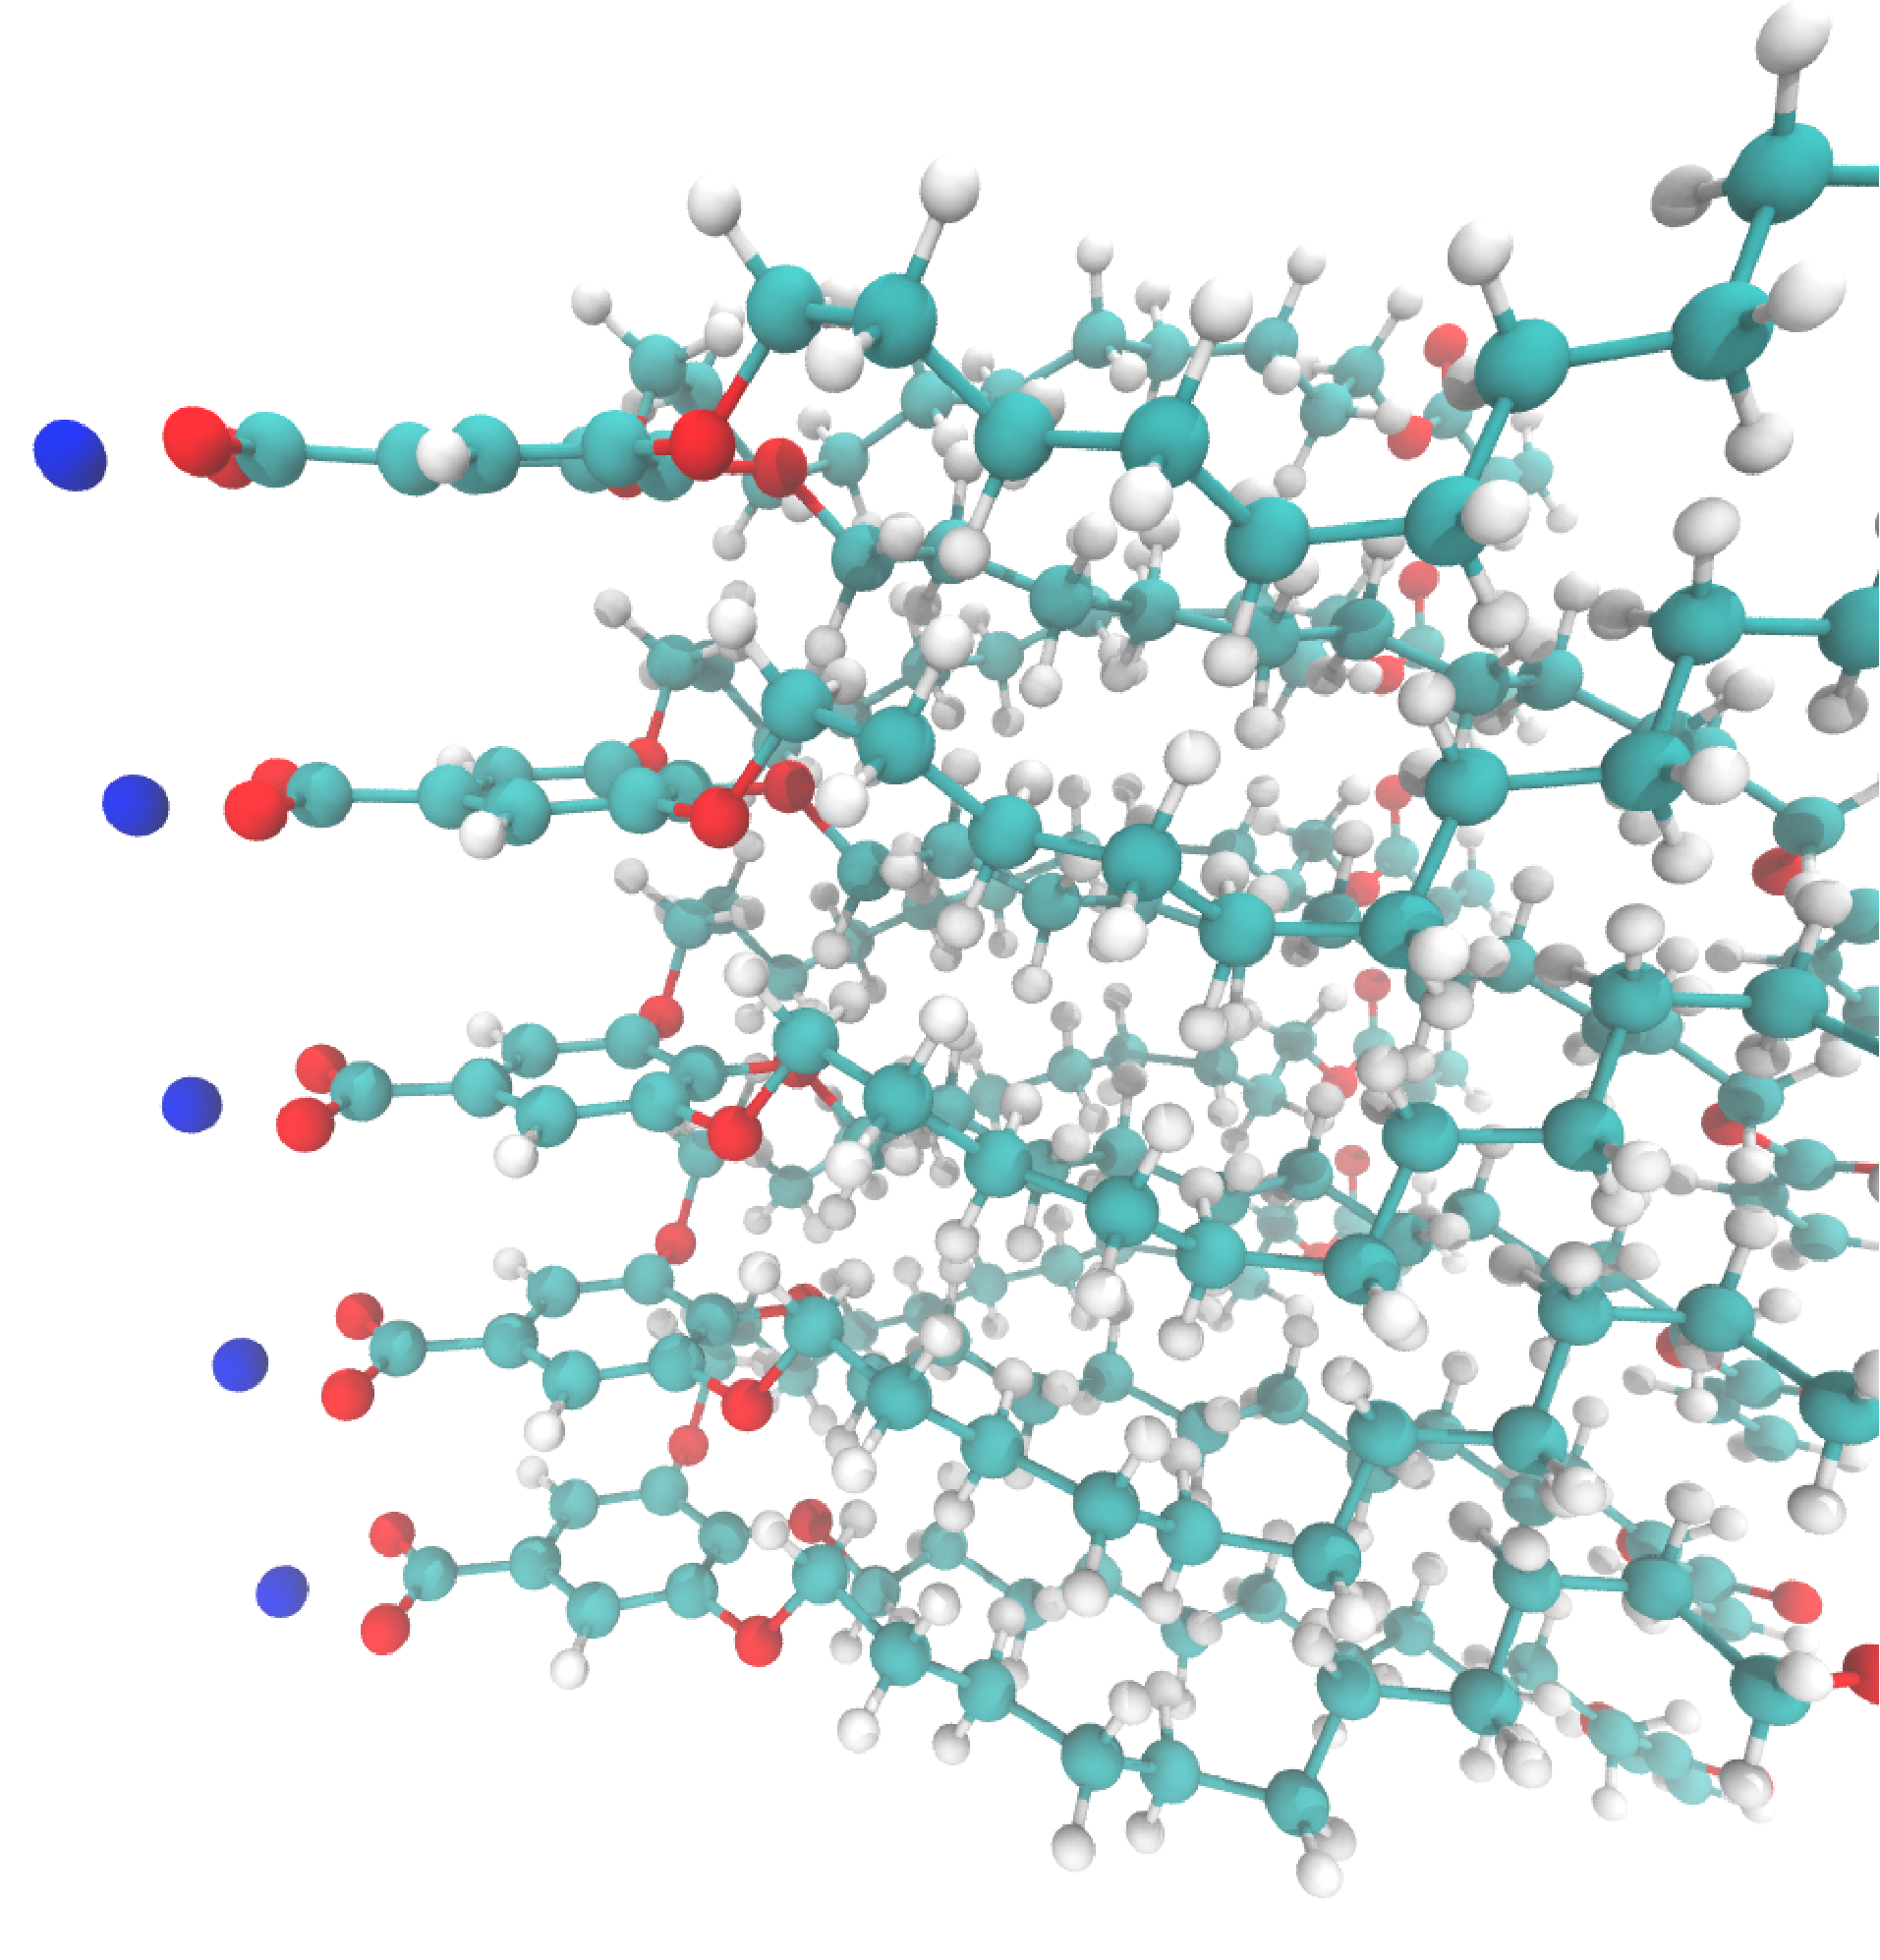
\includegraphics[width=\linewidth]{stacked_monomers.pdf}
  \caption{}
  \end{subfigure}
  \begin{subfigure}[t]{0.35\textwidth}
  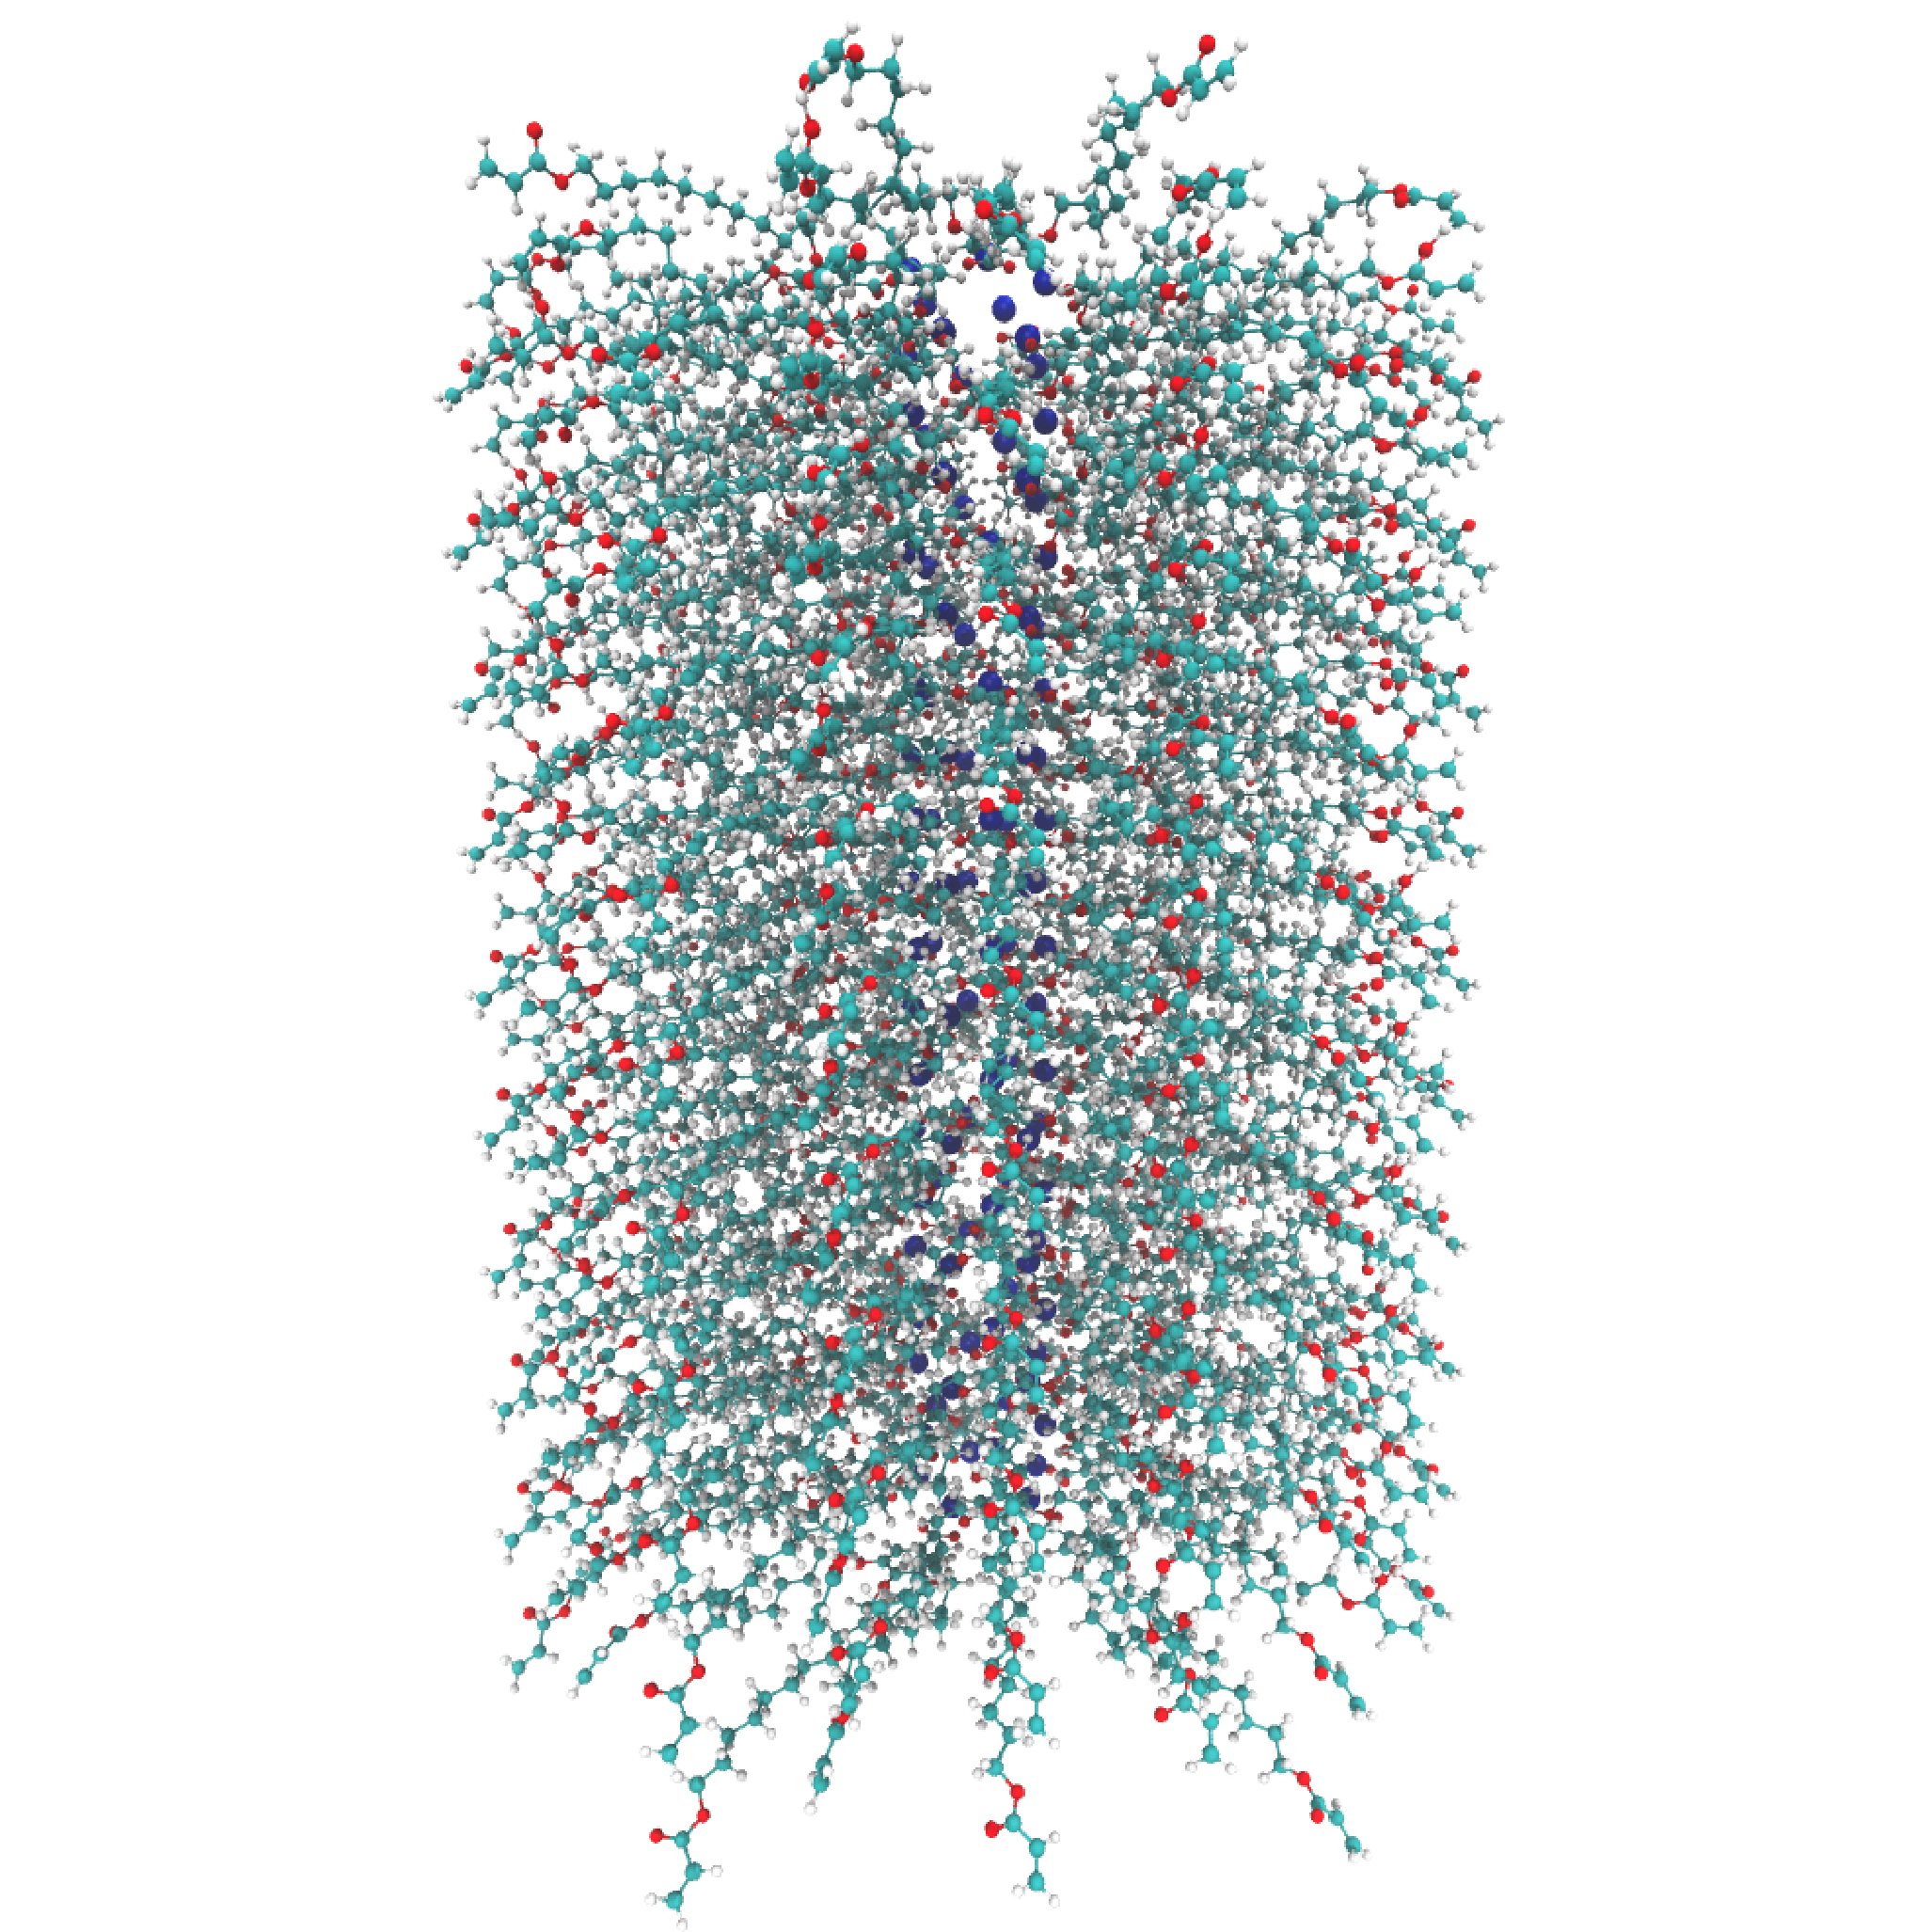
\includegraphics[width=\linewidth]{initial_pore.pdf}
  \caption{}
  \end{subfigure}
  \begin{subfigure}[t]{0.45\textwidth}
  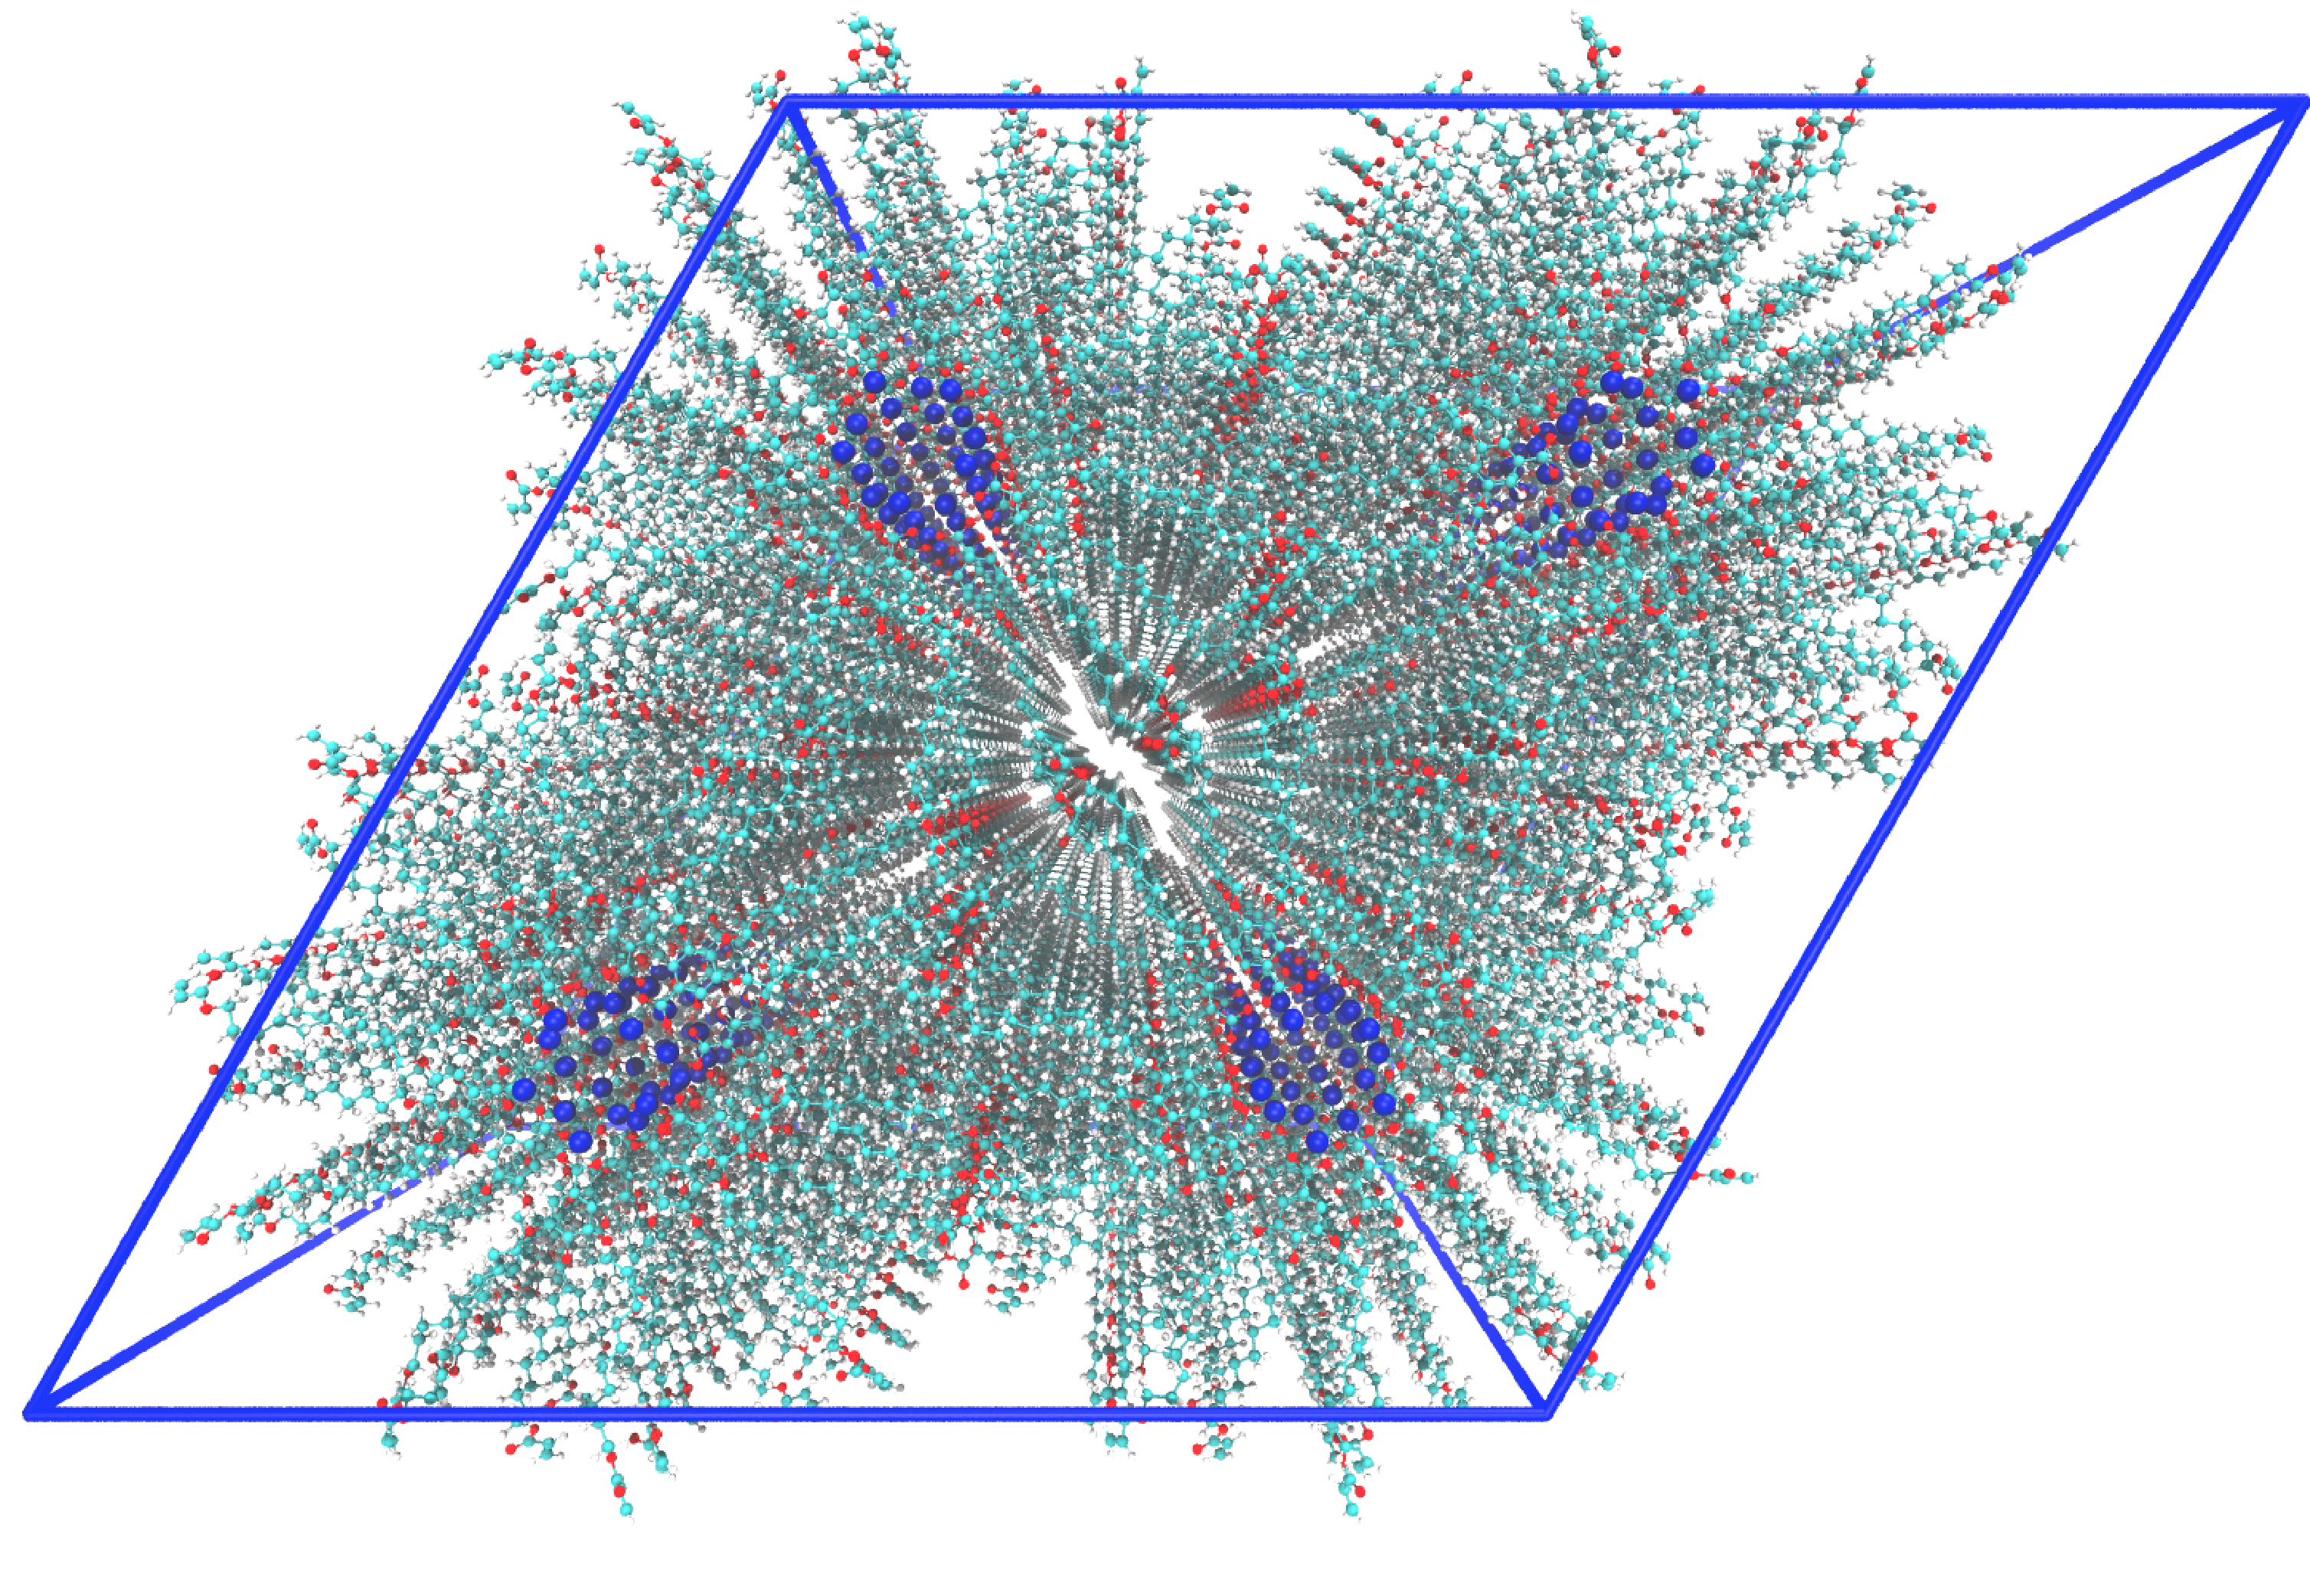
\includegraphics[width=\linewidth]{initial_unit_cell.pdf}
  \caption{}
  \end{subfigure}
  %MRSF: I think this can be put in Supporting Information (we will get pushback to make this paper shorter, this is a good candidate)
  \caption{(a) We parameterized a single monomer and annealed it to produce a low-energy
		configuration. (b) We assembled monomers into columns by stacking them on top of each 
		other. (c) We duplicated each column and rotated them to create hydrophilic pore centers.
		We chose to stack twenty monomers into each column. (d) We duplicated the pores and 
		placed them into a monoclinic unit cell with hexagonal symmetry.}\label{fig:build_procedure}
  \end{figure}

  \section{Number of monomers per column}\label{section:monomers_per_column}
  
  We chose to build all systems using 20 monomers per column, i.e. for a simulation with 5 columns around each pore, there are 100 monomers per pore, and 400 monomers per simulation.  We made this choice
  by considering a number of factors that directly affect the quality of our results. 
  Clearly, choosing a smaller number of layers will cause the system to suffer from 
  larger finite size effects. Even in our 20 monomer-per-column system, axial correlations
  between stacked monomers persist throughout the entire correlation function (see
  Figure~\ref{M-fig:correlation} of the main text). The correlation function of the system which we
  built with 40 monomers per column is very similar to that created with 20 monomers
  per columns (continues to oscillate for its full length
  (Figure~\ref{fig:tall_correlation_full})). If we continue adding monomers, the 
  correlation function will eventually fully decay but it is not worth the 
  computational expense. We do find that the correlation lengths calculated from 20
  monomer per column simulations are in sufficient agreement with experiment. 

  \begin{figure}[!htb]
  \centering
  \begin{subfigure}{0.45\textwidth}
  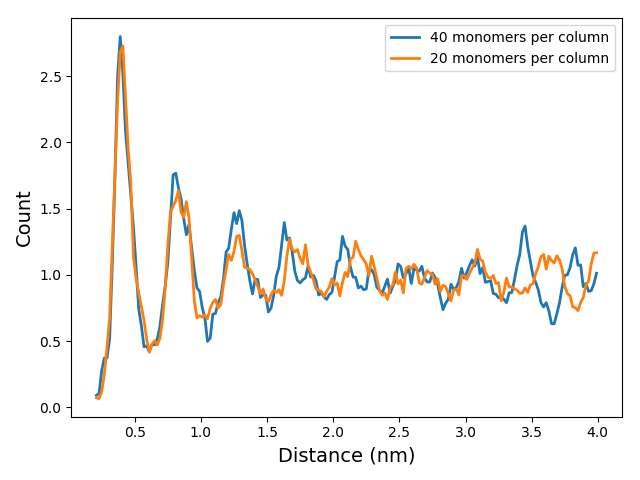
\includegraphics[width=\textwidth]{z_correlation_overlay.png}
  \caption{}\label{fig:z_correlation_overlay}
  \end{subfigure}
  \begin{subfigure}{0.45\textwidth}
  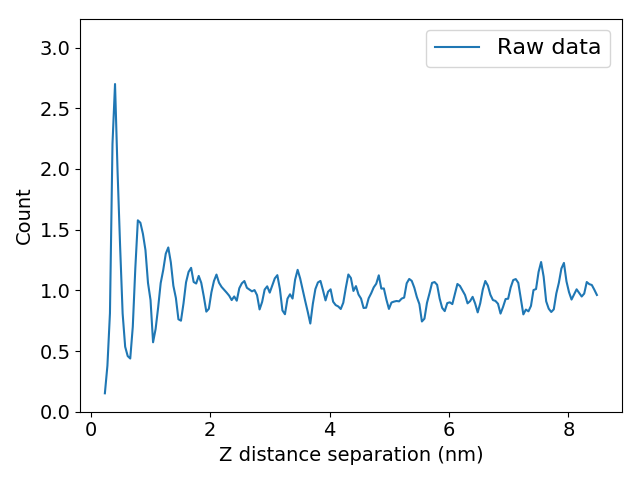
\includegraphics[width=\textwidth]{tall_correlation_full.png}
  \caption{}\label{fig:tall_correlation_full}
  \end{subfigure}
  \caption{(a) The correlation functions generated from ordered basin sandwiched 
  configurations are nearly the same when the $z$-dimension of the system is doubled.
  (b) Oscillations persist throughout the length of the correlation function for the
  sandwiched system in the ordered basin built with 40 monomers per column. The full
  system is ca. 17 nm tall so the full correlation function covers half this length
  since periodicity forces the remaining length to be its mirror image.}\label{fig:correlation_functions}
  \end{figure}
  
  We may be able to simulate systems using less than 20 monomers per column, but chose
  to use 20 since it gives fairly good resolution when simulating X-ray diffraction 
  patterns. The size of the Fourier space bin in each dimension is determined by 
  $\dfrac{2\pi}{L}$ where L is the length of a given box vector. The $z$-box vector 
  for 20 monomer-per-column systems is $\approx$ 85 \AA which means we will see 
  a reciprocal space resolution of 0.074 \AA$^{-1}$ in the z direction. Further decreasing
  the resolution would increase the noise in the simulated patterns and make it more
  difficult to measure the intensity of reflections of interest.

  \section{Initial Configuration Dependence}\label{section:initial_config_dependence}

  We addressed any major dependence on initial configuration in the main text.
  There we showed that systems are stable when made with 4, 5, 6, 7, and 8
  columns per pore. We also showed that systems are stable when monomer head
  groups are oriented in the parallel displaced and sandwiched configurations
  (see Figure~\ref{fig:stacking}). Our model is most consistent with experiment
  when built with 5 columns per pore, with monomers stacked 3.7 \AA~apart in 
  the parallel displaced configuration. 

  There are three other parameters whose choice may influence the equilibrium
  structure: initial pore spacing, initial pore radius and initial stacking distance
  between monomers. Here we show the results of a sensitivity analysis performed
  on the three parameters. To reduce the size of the sensitivity analysis, we
  only tested systems built with 5 columns per pore with monomers stacked in 
  the parallel displaced configuration. We equilibrated all systems according
  to the dry equilibration procedure.

  \subsection{Initial pore spacing}\label{section:initial_pore_spacing}

  We tested five different initial pore spacings, defined as the
  distance between the central axis of each pore with all others
  (Figure~\ref{fig:p2p_diagram}). To reduce the number of variables, we held the
  pore radius constant, at 5 \AA~and the distance between layers at 3.7 \AA~since
  those were the values used in our optimal system in the main text. We
  prioritized ensuring that resulting configurations maintain the expected
  hexagonal symmetry. If initial pore spacing is too small, we observe repulsion
  between columns which disrupts equilibration. If the pore spacing is too large
  the pores squeeze together, but in a distorted hexagonal array because the $xy$
  initial translation of the pores is somewhat erratic. 

%	  If the initial pore spacing is chosen to be
%	  too small, pore columns abruptly repel each other as soon as they are able to
%	  overcome the restraining potential present as part of the dry equilibration
%	  procedure. We avoided using systems that exhibit this behavior since the
%	  behavior increases the chances of a system to become kinetically trapped in an
%	  undesired metastable free energy basin.  

	\begin{enumerate}

	\item 39 \AA~: We tested a pore spacing of 39 \AA~in order to
	have a test system with an initial spacing below the experimental value. As soon
	as the restraining potential switches to 56 kJ mol$^{-1}$ nm$^{-2}$, the
	columns are able to repel resulting in a large jump in pore spacing
	(Figure~\ref{fig:p2p_39}). %After 400 ns, the pore spacing is 4.05 $\pm$ 0.17 nm.
%		There is a large uncertainty in this value because the 1-4 pore spacing
%		(Figure~\ref{fig:p2p_diagram}) deviates significantly from all other pore
%		spacings. The 1-4 pore spacing is 4.31 nm while the average of all other pore
%		spacings is 3.96 nm. The system deviates from hexagonal geometry and is trending
%                towards cubic packing.

		\item 41 \AA~: We chose to test a pore spacing of 41 \AA~since
	it closely matches the experimental pore spacing. Again, we observe abrupt
	repulsion of columns once the restraining potential is switched to 56 kJ
	mol$^{-1}$ nm$^{-2}$ (Figure~\ref{fig:p2p_41}). %After 400 ns, the
%		average pore spacing settles below the experimental value at 4.07 $\pm$ 0.21
%		nm. Again, a large uncertainty in this value occurs because the 1-4 pore spacing
%		(Figure~\ref{fig:p2p_diagram}) deviates significantly from all other pore
%		spacings. The 1-4 pore spacing is 4.44 nm while the average of all other pore
%		spacings is 3.96 nm. 

		\item 45 \AA~: A pore spacing of 45 \AA~is about 10\% larger
	than the experimental value. This systems exhibits the smallest response to our 
 		equilibration procedure (Figure~\ref{fig:p2p_45}) and we chose to use this
        value for all our simulations in the main text.
        %The equilibrated pore spacing is 4.23 $\pm$ 0.03 nm.
	%The system maintains hexagonal symmetry and exhibits the lowest uncertainty in
	%pore spacing. We chose to use this value for all our simulations in the main
	%text. 

	\item 50 \AA~: We tested a pore spacing of 50 \AA, about 20\%
	larger than the experimental value. Once the restraining potential reaches 56
	kJ mol$^{-1}$ nm$^{-2}$, the pore spacing begins to decrease rapidly, following
	a linear trend (Figure~\ref{fig:p2p_50}).
%		After 400 ns, the average pore spacing is 4.37 $\pm$ 0.13 nm.
%		There is a large
 %               uncertainty with this value because, again, the array of pores deviates from 
 %               hexagonal character. Using Figure ~\ref{fig:p2p_diagram} as a reference, pore 
  %              2 drifts outward from the array and forces the 1-4 distance to shrink in 
   %             response.
                
	\item 55 \AA~: We tested a pore spacing of 55 \AA~which is at
	a distance where monomers in each pore no longer intersect those of adjacent pores. Once
	the restraining potential reaches 56 kJ mol$^{-1}$ nm$^{-2}$, the pore spacing
	changes erratically until it begins to settle when the force constants are
	below 3 kJ mol$^{-1}$ nm$^{-2}$ (Figure~\ref{fig:p2p_55}). We recommend
	avoiding a system such as this where vacuum gaps between pore columns are
	introduced unnecessarily. 
	%The system equilibrates to a pore spacing of 4.27
    %$\pm$ 0.18 nm. The 1-2 pore spacing is the outlier in this case with a pore
    %spacing of 3.99 \AA~ which distorts the hexagonal array. 

	\end{enumerate} 

	% BJC: Could put vertical lines to indicate where position restraint values are reduced
  	\begin{figure}[!htb]
	\centering
	\begin{subfigure}{0.3\textwidth}
	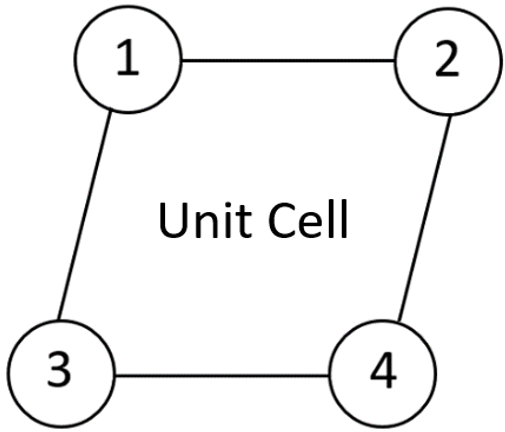
\includegraphics[width=\textwidth]{p2p_diagram.png}
	\caption{}~\label{fig:p2p_diagram}
%		\caption{In a perfect hexagonal, there are 5 distances that should be exactly
%		equal. As pictured in this diagram the distance from 1-2, 1-3, 1-4, 2-4, and 3-4
%		are the same.}~\label{fig:p2p_diagram}
  	\end{subfigure} 
	\begin{subfigure}{0.3\textwidth}
		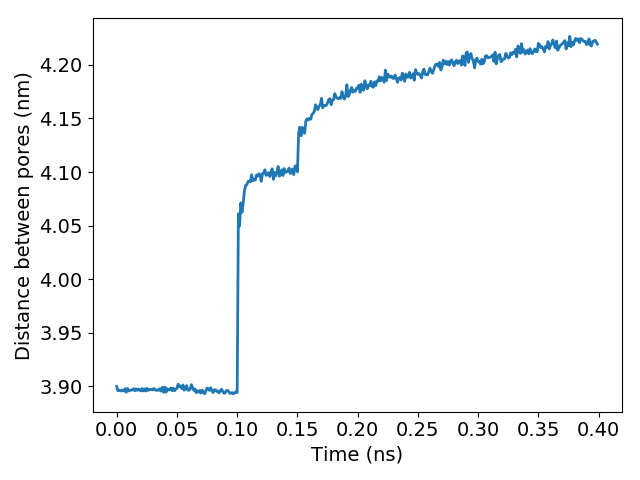
\includegraphics[width=\textwidth]{p2p_39.png}\quad
		\vspace{-1.25em}
		\caption{39 \AA~initial pore spacing}~\label{fig:p2p_39}
	\end{subfigure}
	\begin{subfigure}{0.3\textwidth}
		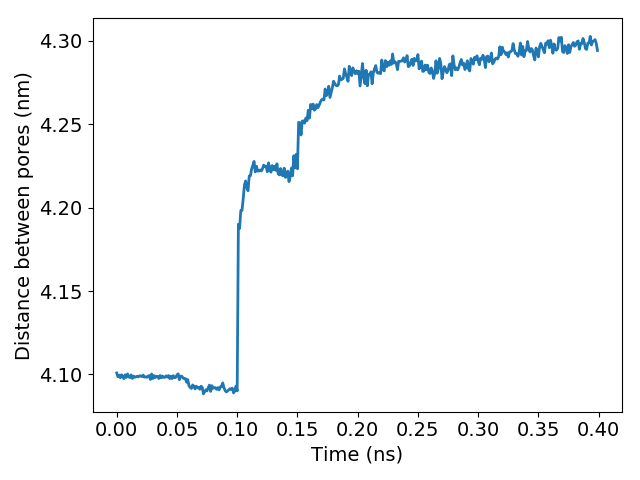
\includegraphics[width=\textwidth]{p2p_41.png}\quad
		\vspace{-1.25em}
		\caption{41 \AA~initial pore spacing}~\label{fig:p2p_41}
	\end{subfigure}
	\begin{subfigure}{0.3\textwidth}
		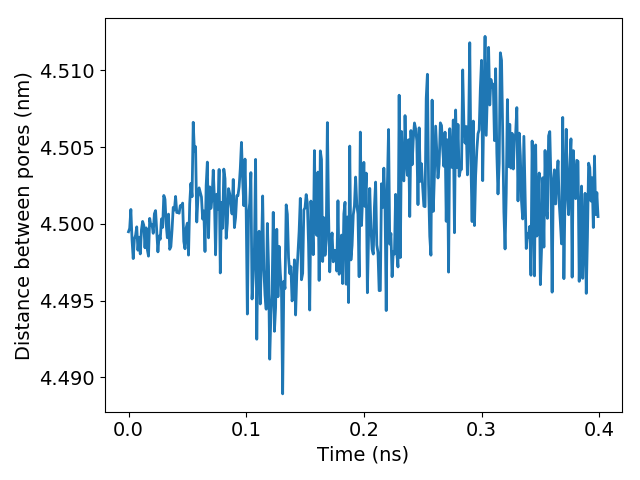
\includegraphics[width=\textwidth]{p2p_45.png}
		\vspace{-1.25em}
		\caption{45 \AA~initial pore spacing}~\label{fig:p2p_45}
	\end{subfigure}
	\begin{subfigure}{0.3\textwidth}
		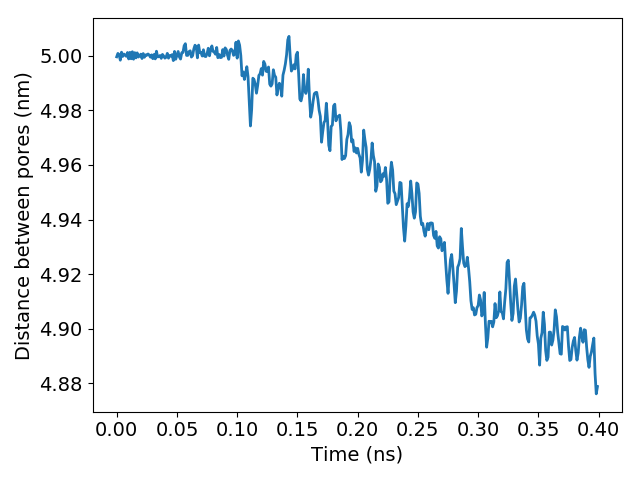
\includegraphics[width=\textwidth]{p2p_50.png}\quad	
		\vspace{-1.25em}
		\caption{50 \AA~initial pore spacing}~\label{fig:p2p_50}
	\end{subfigure}
	\begin{subfigure}{0.3\textwidth}
		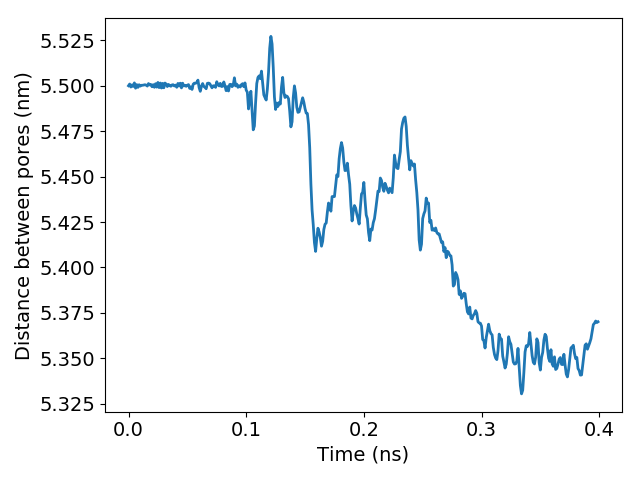
\includegraphics[width=\textwidth]{p2p_55.png}
		\vspace{-1.25em}
		\caption{55 \AA~initial pore spacing}~\label{fig:p2p_55}
	\end{subfigure}
	\caption{(a) In a perfect hexagonal array, there are 5 distances that should be exactly
	equal. As pictured in this diagram the distance from 1-2, 1-3, 1-4, 2-4, and 3-4
	are the same. All plots in (b)--(f) are the average of these distances and represent
	the pore spacing during the restrained portion of the dry equilibration procedure.
	Every 50 ps (0.05 ns) we reduce the force constant on the position restraints according to the sequence: 1000000,
	3162, 56, 8, 3, 2, 1, 0 kJ mol$^{-1}$ nm$^{-2}$. When we chose an initial pore
	spacing below experimental value (b) or at the experimental value (c), there
	is an abrupt change in pore spacing when the position restraints are reduced to 56 kJ
	mol$^{-1}$ nm$^{-2}$. When we initially position pores 45 \AA~apart (d) the pore spacing
	remains relatively stable. When we initially place pores 50 \AA~apart (e), the pore
	spacing decreases nearly linearly once the restraints are reduced to 56 kJ
	mol$^{-1}$ nm$^{-2}$. When we initially place pores 55 \AA~apart (f), so that monomers
	do not intersect with adjacent pores, and position restraints are reduced to 56
	kJ mol$^{-1}$ nm$^{-2}$, the pore spacing changes erratically before stabilizing
	when force constants are reduced below 3 kJ mol$^{-1}$ nm$^{-2}$. } 
	\label{fig:p2p}
  \end{figure}

  \subsection{Initial pore radius}\label{section:initial_pore_radius}

  We tested 3 different pore radii, defined as shown in
  Figure~\ref{fig:pore_radius_illustration}. For each system, we held the initial
  pore spacing constant at 45 \AA~and the initial stacking distance between monomers
  constant at 3.7 \AA. Equilibrated values of pore radii are presented in
  Table~\ref{table:radii}. The pore radius in each simulation frame is calculated
  as the average distance of all carbonyl carbons (see
  Figure~\ref{fig:pore_radius_illustration}) from their associated pore center.
  We generated statistics for the pore radii reported from the time series
  representing the average pore radius at each frame. We detected equilibration
  as described in Section~\ref{M-method:equil_time} of the main text. We 
  calculated the average and standard deviation of pore radii using only data 
  points collected after equilibration was detected.

  \begin{enumerate}

  \item 2.5 \AA~: The smallest pore radius that we can achieve
  before energy minimization becomes problematic is 2.5 \AA. After being run
  through the full dry equilibration procedure, the average pore radius is 0.40
  $\pm$ 0.01 \AA.

  \item 5 \AA~: We tested a pore radius of 5 \AA~because it is
  slightly larger than the equilibrated pore radius of the system simulated with
  an initial pore radius of 2.5 \AA. After being run through the full dry
  equilibration procedure, the average pore radius is 0.42 $\pm$ 0.01 \AA, which
  agrees with the 2.5 \AA~configuration within uncertainty. 

  \item 8 \AA~: The largest pore radius that can achieved before
  energy minimization becomes problematic is 8 \AA. One should use caution with
  such a structure because of the relatively large vacuum space that is created
  in the pore region of the initial configuration. After being run through the
  full dry equilibration procedure, we see a combination of cylindrical and
  slit-like pores (Figure~\ref{fig:slits}). Measuring the pore radius of this
  system does not have a concrete meaning since slits do not have a single
  radius, but its calculated value is still reported in Table ~\ref{table:radii}. We
  are wary of such a non-symmetric structure and choose not to use a pore radius
  of 8 \AA~for our starting configurations. 
  
  \end{enumerate}

  \begin{table}[h]
  \centering
  \begin{tabular}{cc}
  \toprule
  Initial Pore Radius & Equilibrated Pore Radius \\
  \midrule
  2.5 \AA & $4.0 \pm 0.1$ \AA \\
  5 \AA   & $4.2 \pm 0.1$ \AA \\
  8 \AA   & $6.9 \pm 0.1$ \AA \\
  \bottomrule
  \end{tabular}
  \caption{The average pore radii of systems built with an initial pore
	  radius of 2.5 \AA~and 5 \AA~equilibrate to values that agree within error. If
	  the pore radius is too large, slit pores may form.}~\label{table:radii}
  \end{table}

  \begin{figure}[!htb]
  \centering
  \begin{minipage}{0.475\textwidth}
  \centering
  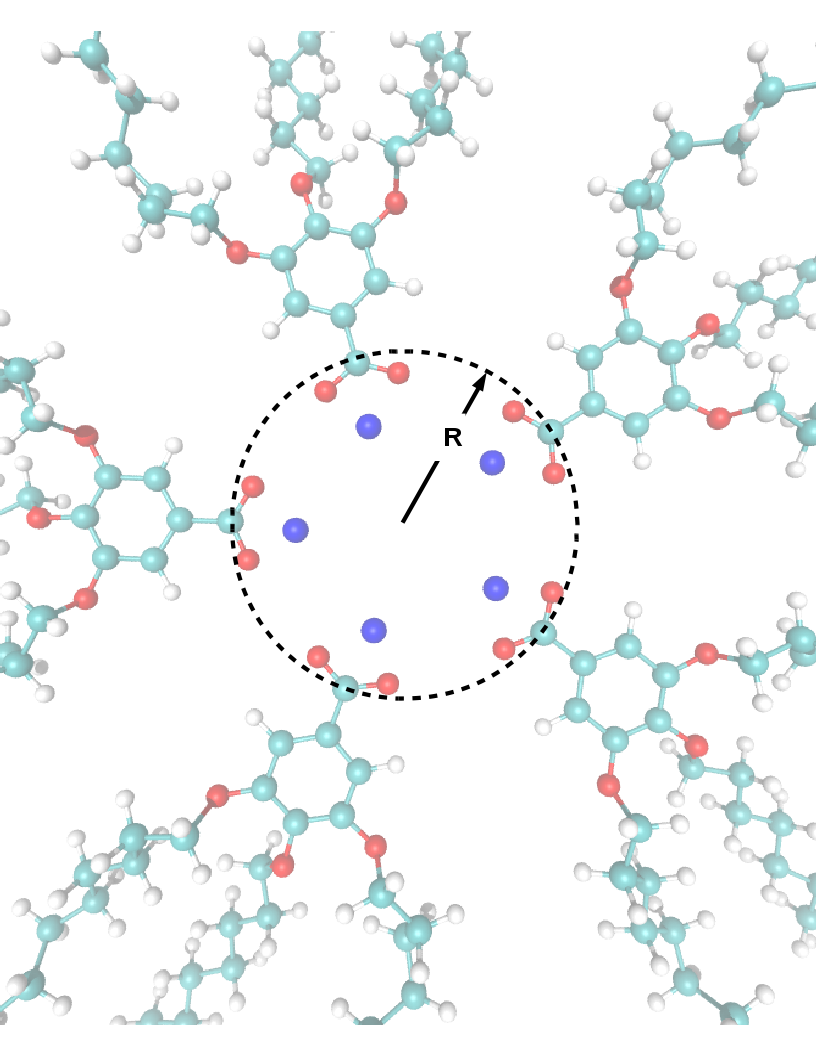
\includegraphics[width=0.8\textwidth]{pore_radius_illustration.png}
  \caption{When creating an initial configuration, we define the pore radius,
  R, based on the distance of the carbonyl carbon from the pore's
  central axis.}~\label{fig:pore_radius_illustration}
  \end{minipage}\qquad
  \begin{minipage}{0.475\textwidth}
  \centering
  \vspace{4em}
  \includegraphics[width=\textwidth]{slit_pores.png}
  \vspace{1em}
  \caption{A system that was built with an initial pore radius of 8~\AA~equilibrates
  to a structure that exhibits both cylindrical and slit-like pores. As pictured 
  here, sodium ions are colored blue, carbon atoms in the aromatic ring of the head 
  group are colored orange and all else is colored cyan.}~\label{fig:slits}
  \end{minipage}
  \end{figure}

  \subsection{Initial stacking distance between monomers}\label{section:initial_dbwl}

  We tested 3 different initial monomer spacings, defined as the $z$-distance
  between the planes of aromatic rings. Systems built with layers
  stacked 3.7 \AA~and 5 \AA~apart are discussed extensively in the main text. We
  also tested a system built with layers stacked 10 \AA~ apart.

  Figure~\ref{fig:dbwl_10} shows the structure of an assembly built
  with an initial layer spacing of 10 \AA~immediately after the restrained
  portion of the equilibration procedure. Since we used position restraints, the
  simulations were run in the NVT ensemble. When layer spacing is large, such as
  this situation, there is a significant amount of vacuum space which the monomer
  attempts to fill. Even if turning pressure control on allows the system to
  recover the geometry of the hexagonal phase, we would likely need much longer
  equilibration times, and it will almost certainly get trapped in a metastable
  configuration that bears no resemblance to the experimental profile. 
 
  \begin{figure}[!htb]
	\centering
	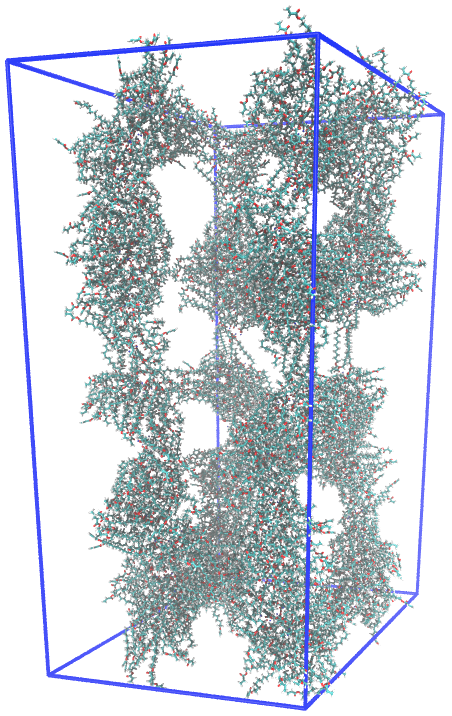
\includegraphics[width=0.3\textwidth]{dbwl_10.png}
	\caption{When layers are initially stacked 10 \AA~apart and the system
                is equilibrated using the dry equilibration procedure, large vacuum gaps
	form as the monomers attempt to fill space.}\label{fig:dbwl_10} 
  \end{figure}

  \clearpage
  \section{Placement of monomer head groups}
  
  The monomer head groups consist of a substituted benzene ring which may participate in
  $\pi-\pi$ stacking interactions. There are three $\pi-\pi$ stacking modes known
  to occur in nature: sandwiched, parallel displaced and T-shaped
  (Figures~\ref{fig:sandwiched}--\ref{fig:tshaped})~\cite{sinnokrot_estimates_2002}.
  We ruled out the T-shaped configuration because its vertical stacking distance is
  inconsistent with experimental spectroscopy. Additionally, steric interactions
  between the bulky alkane tails make this motif unfavorable. We chose to explore
  systems in both the sandwiched and parallel displaced configurations since their
  stacking distances are both consistent with experimental diffraction patterns.
  
  \begin{figure}[!htb]
        \centering
        \begin{subfigure}[b]{0.32\textwidth}
                \centering
                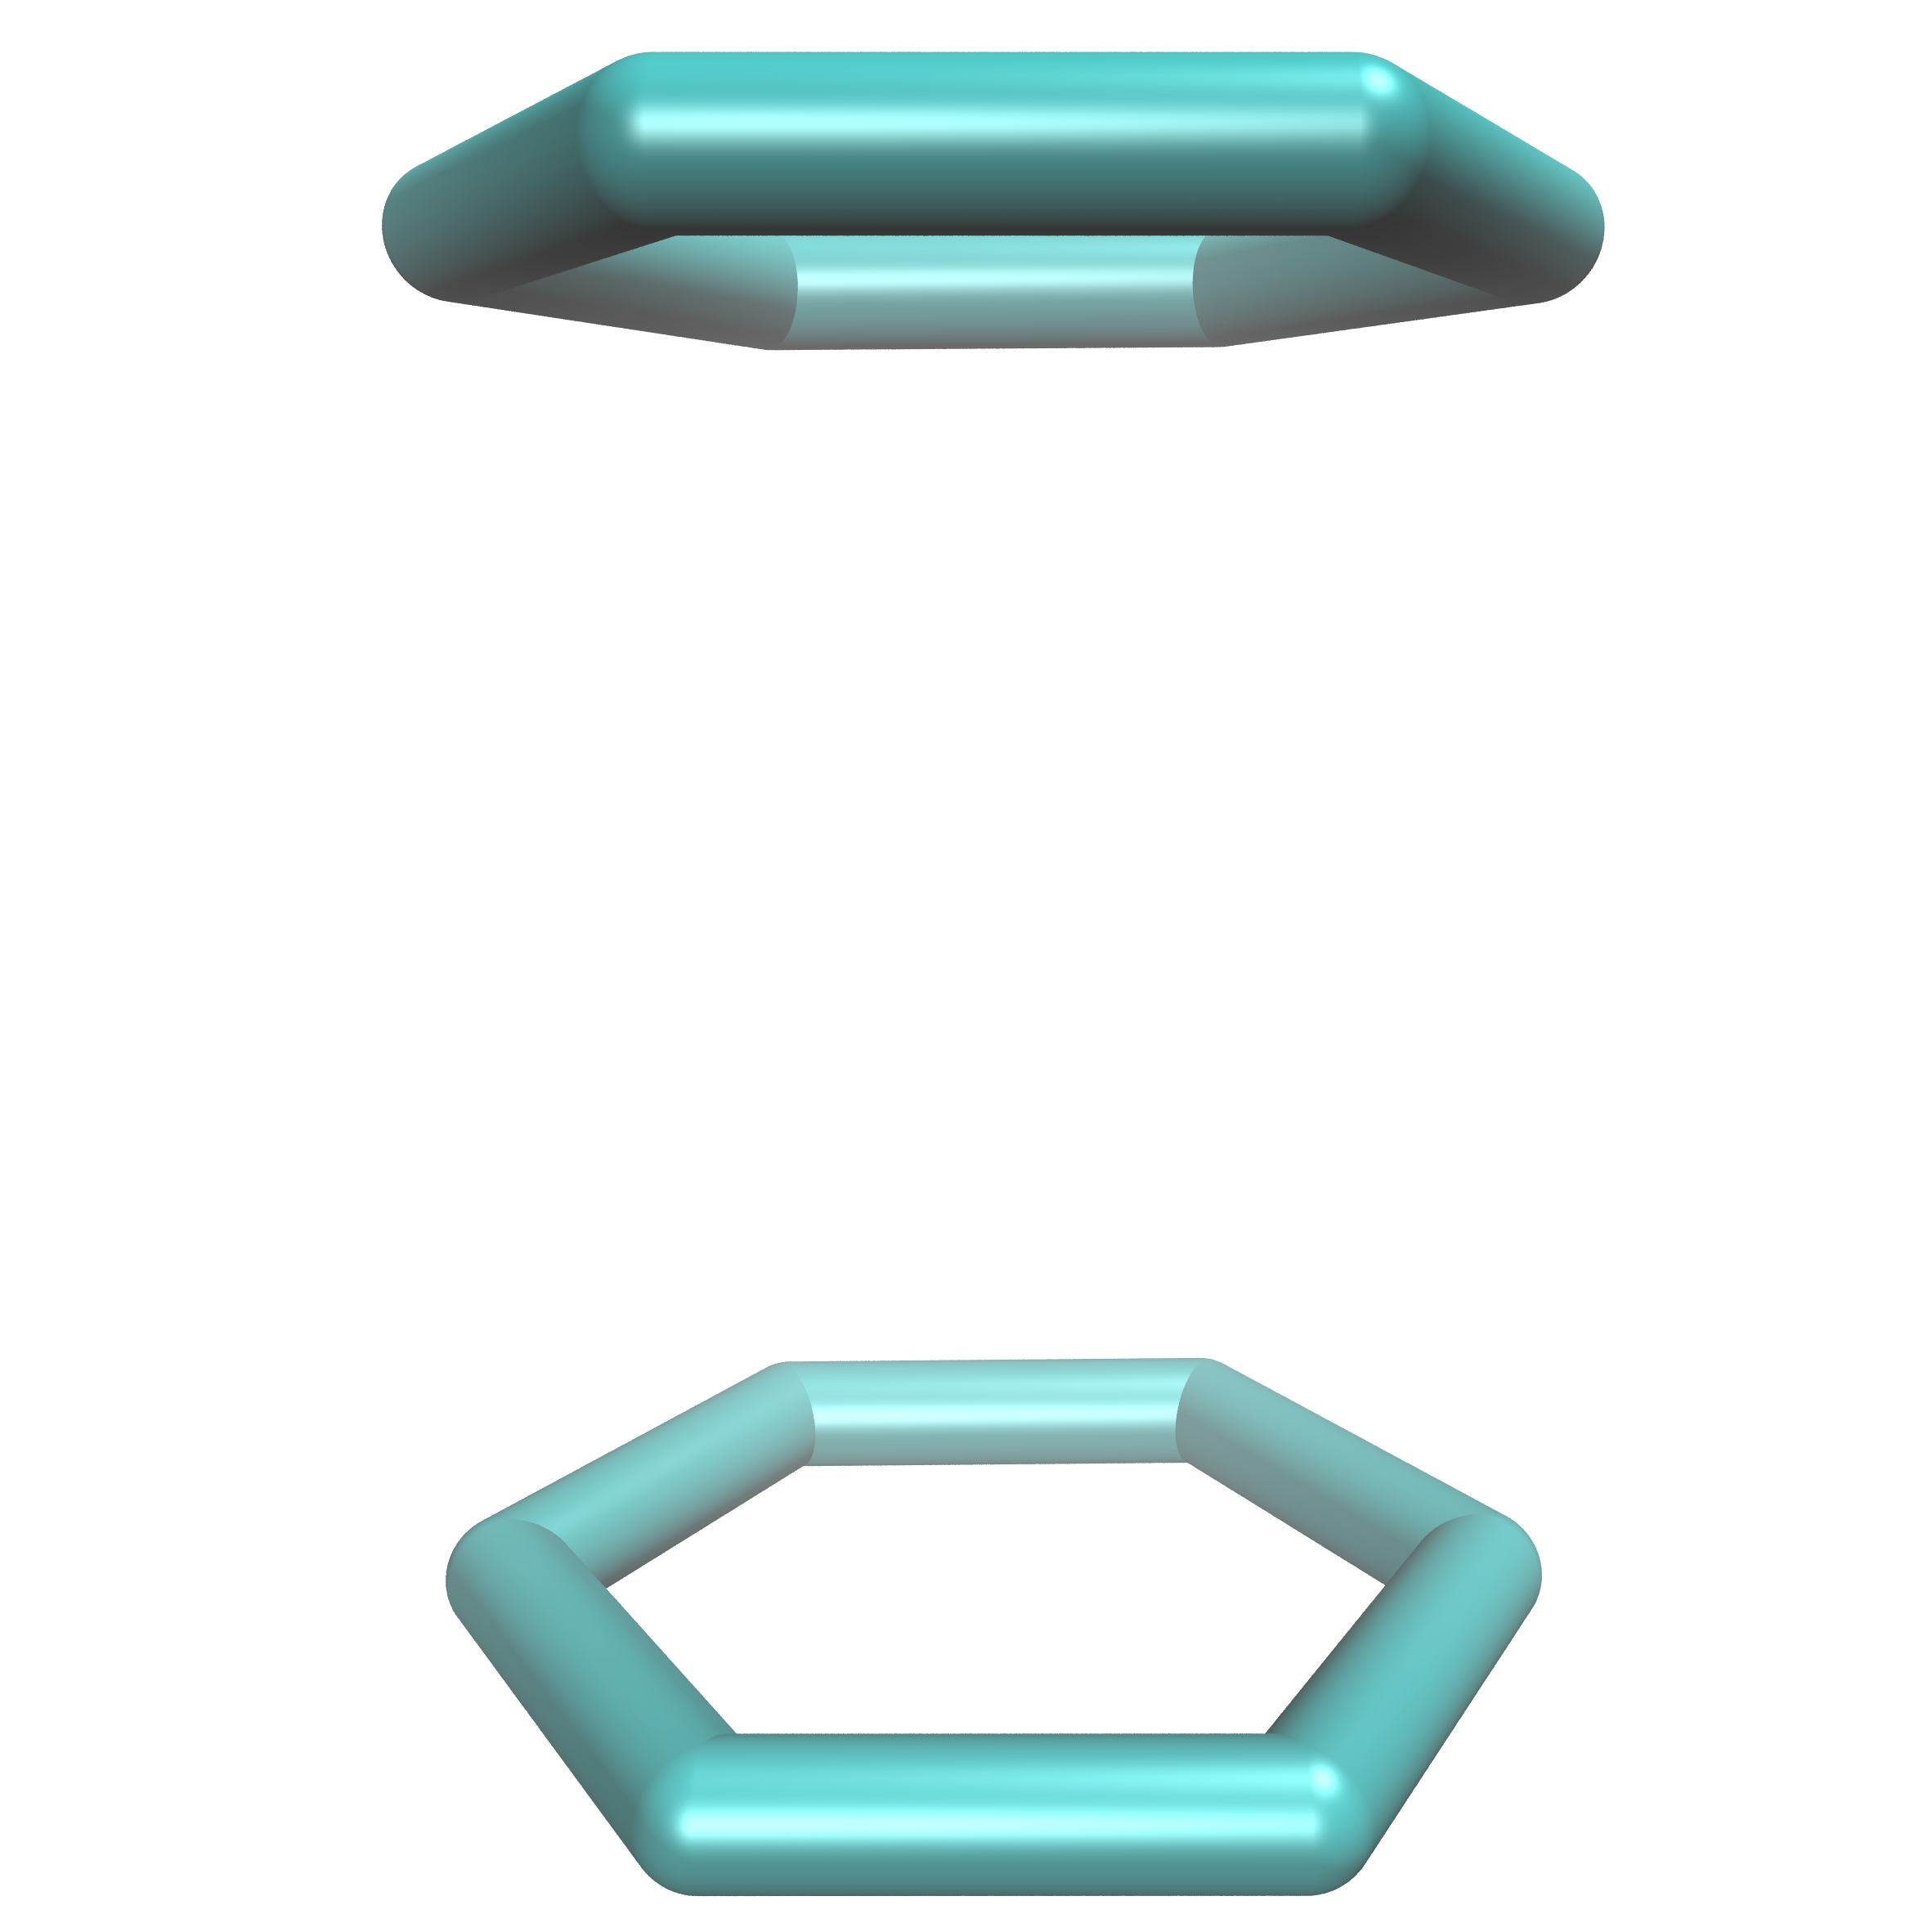
\includegraphics[width=\textwidth]{sandwiched.png}
                \caption{}\label{fig:sandwiched}
        \end{subfigure}
        \begin{subfigure}[b]{0.32\textwidth}
                \centering
                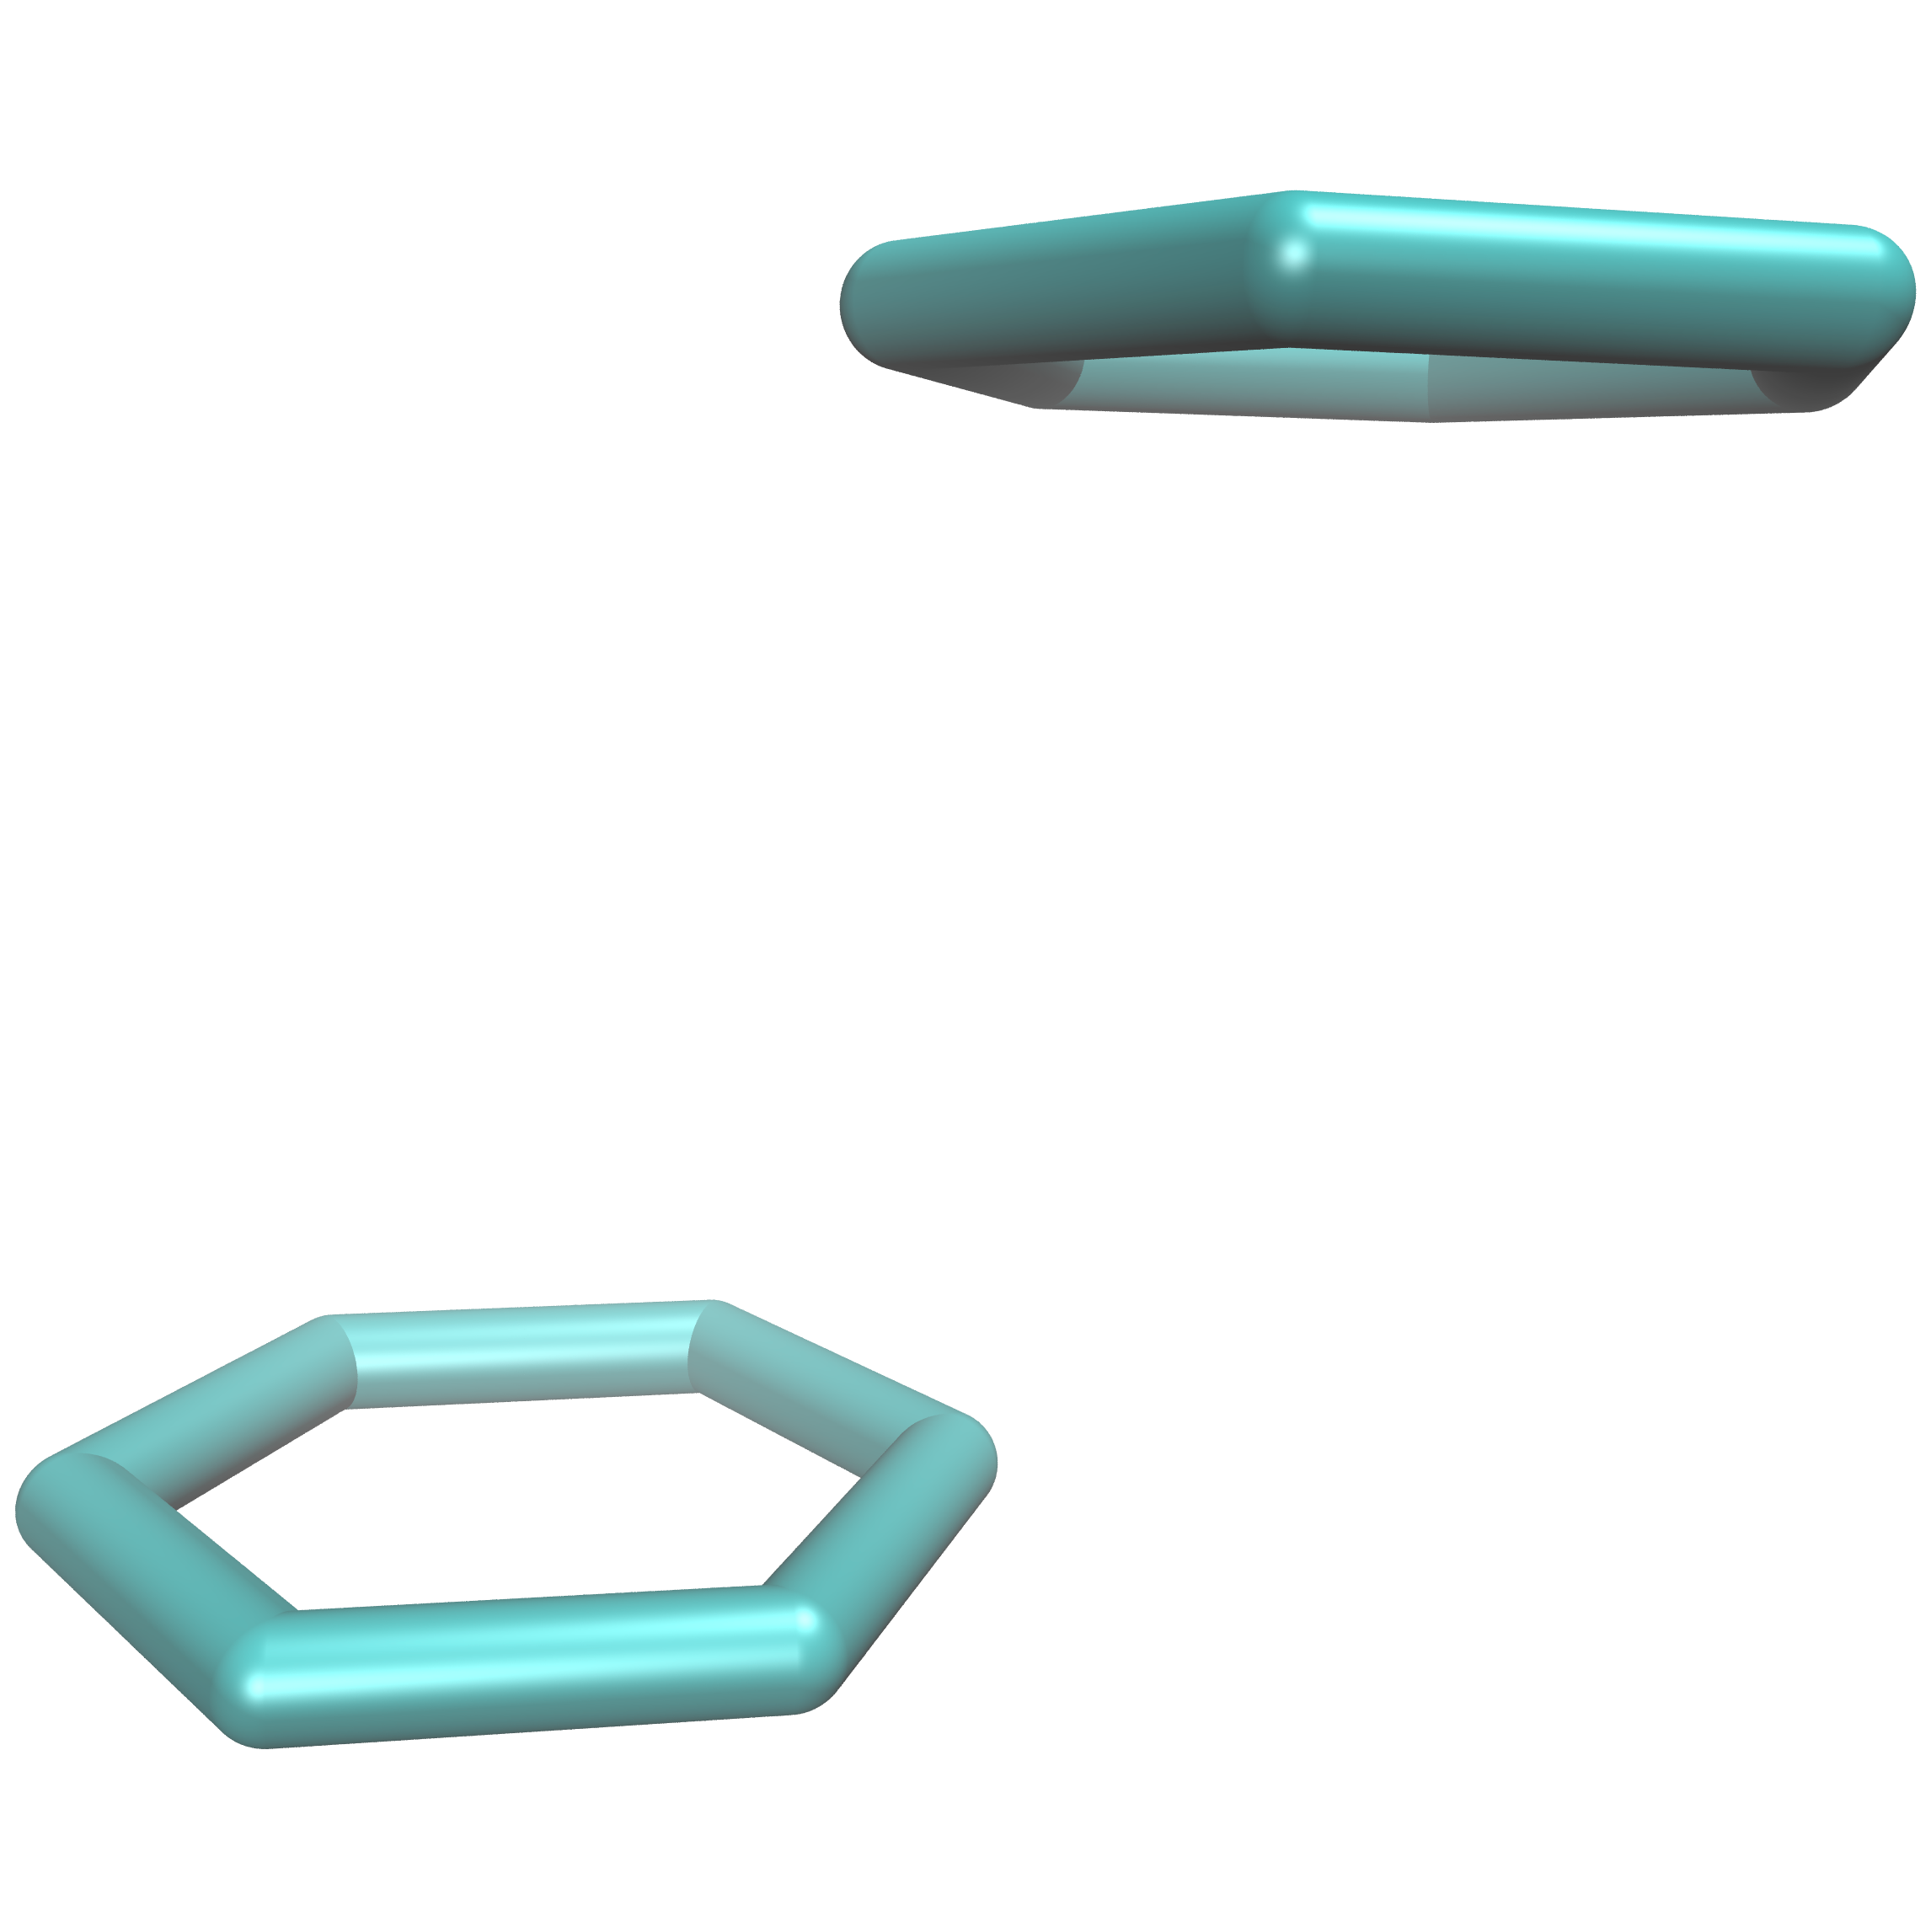
\includegraphics[width=\textwidth]{PD.png}
                \caption{}\label{fig:pd}
        \end{subfigure}
        \begin{subfigure}[b]{0.32\textwidth}
                \centering
                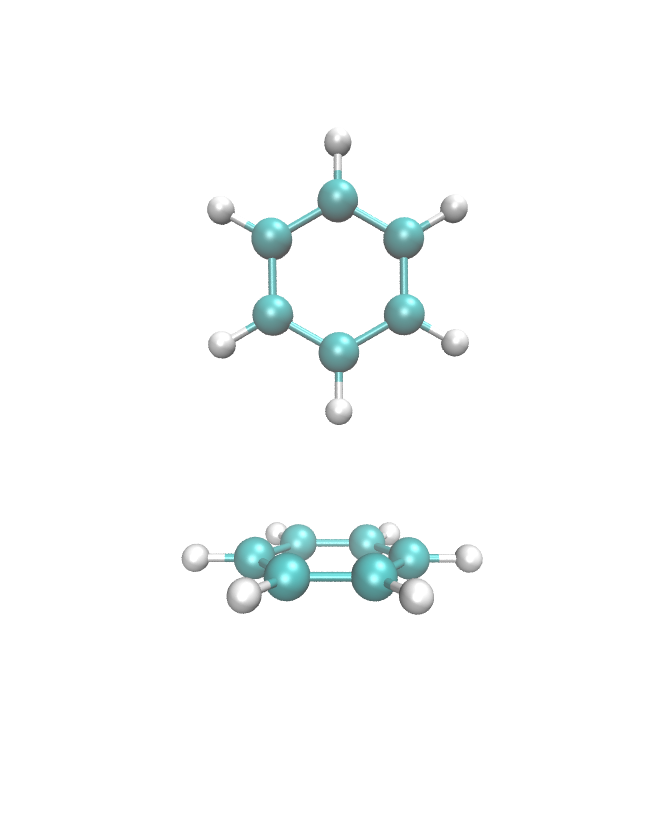
\includegraphics[width=\textwidth]{Tshaped.png}
                \caption{}\label{fig:tshaped}
        \end{subfigure}
        \vskip\baselineskip
        \begin{subfigure}[b]{0.475\textwidth}
                \centering
                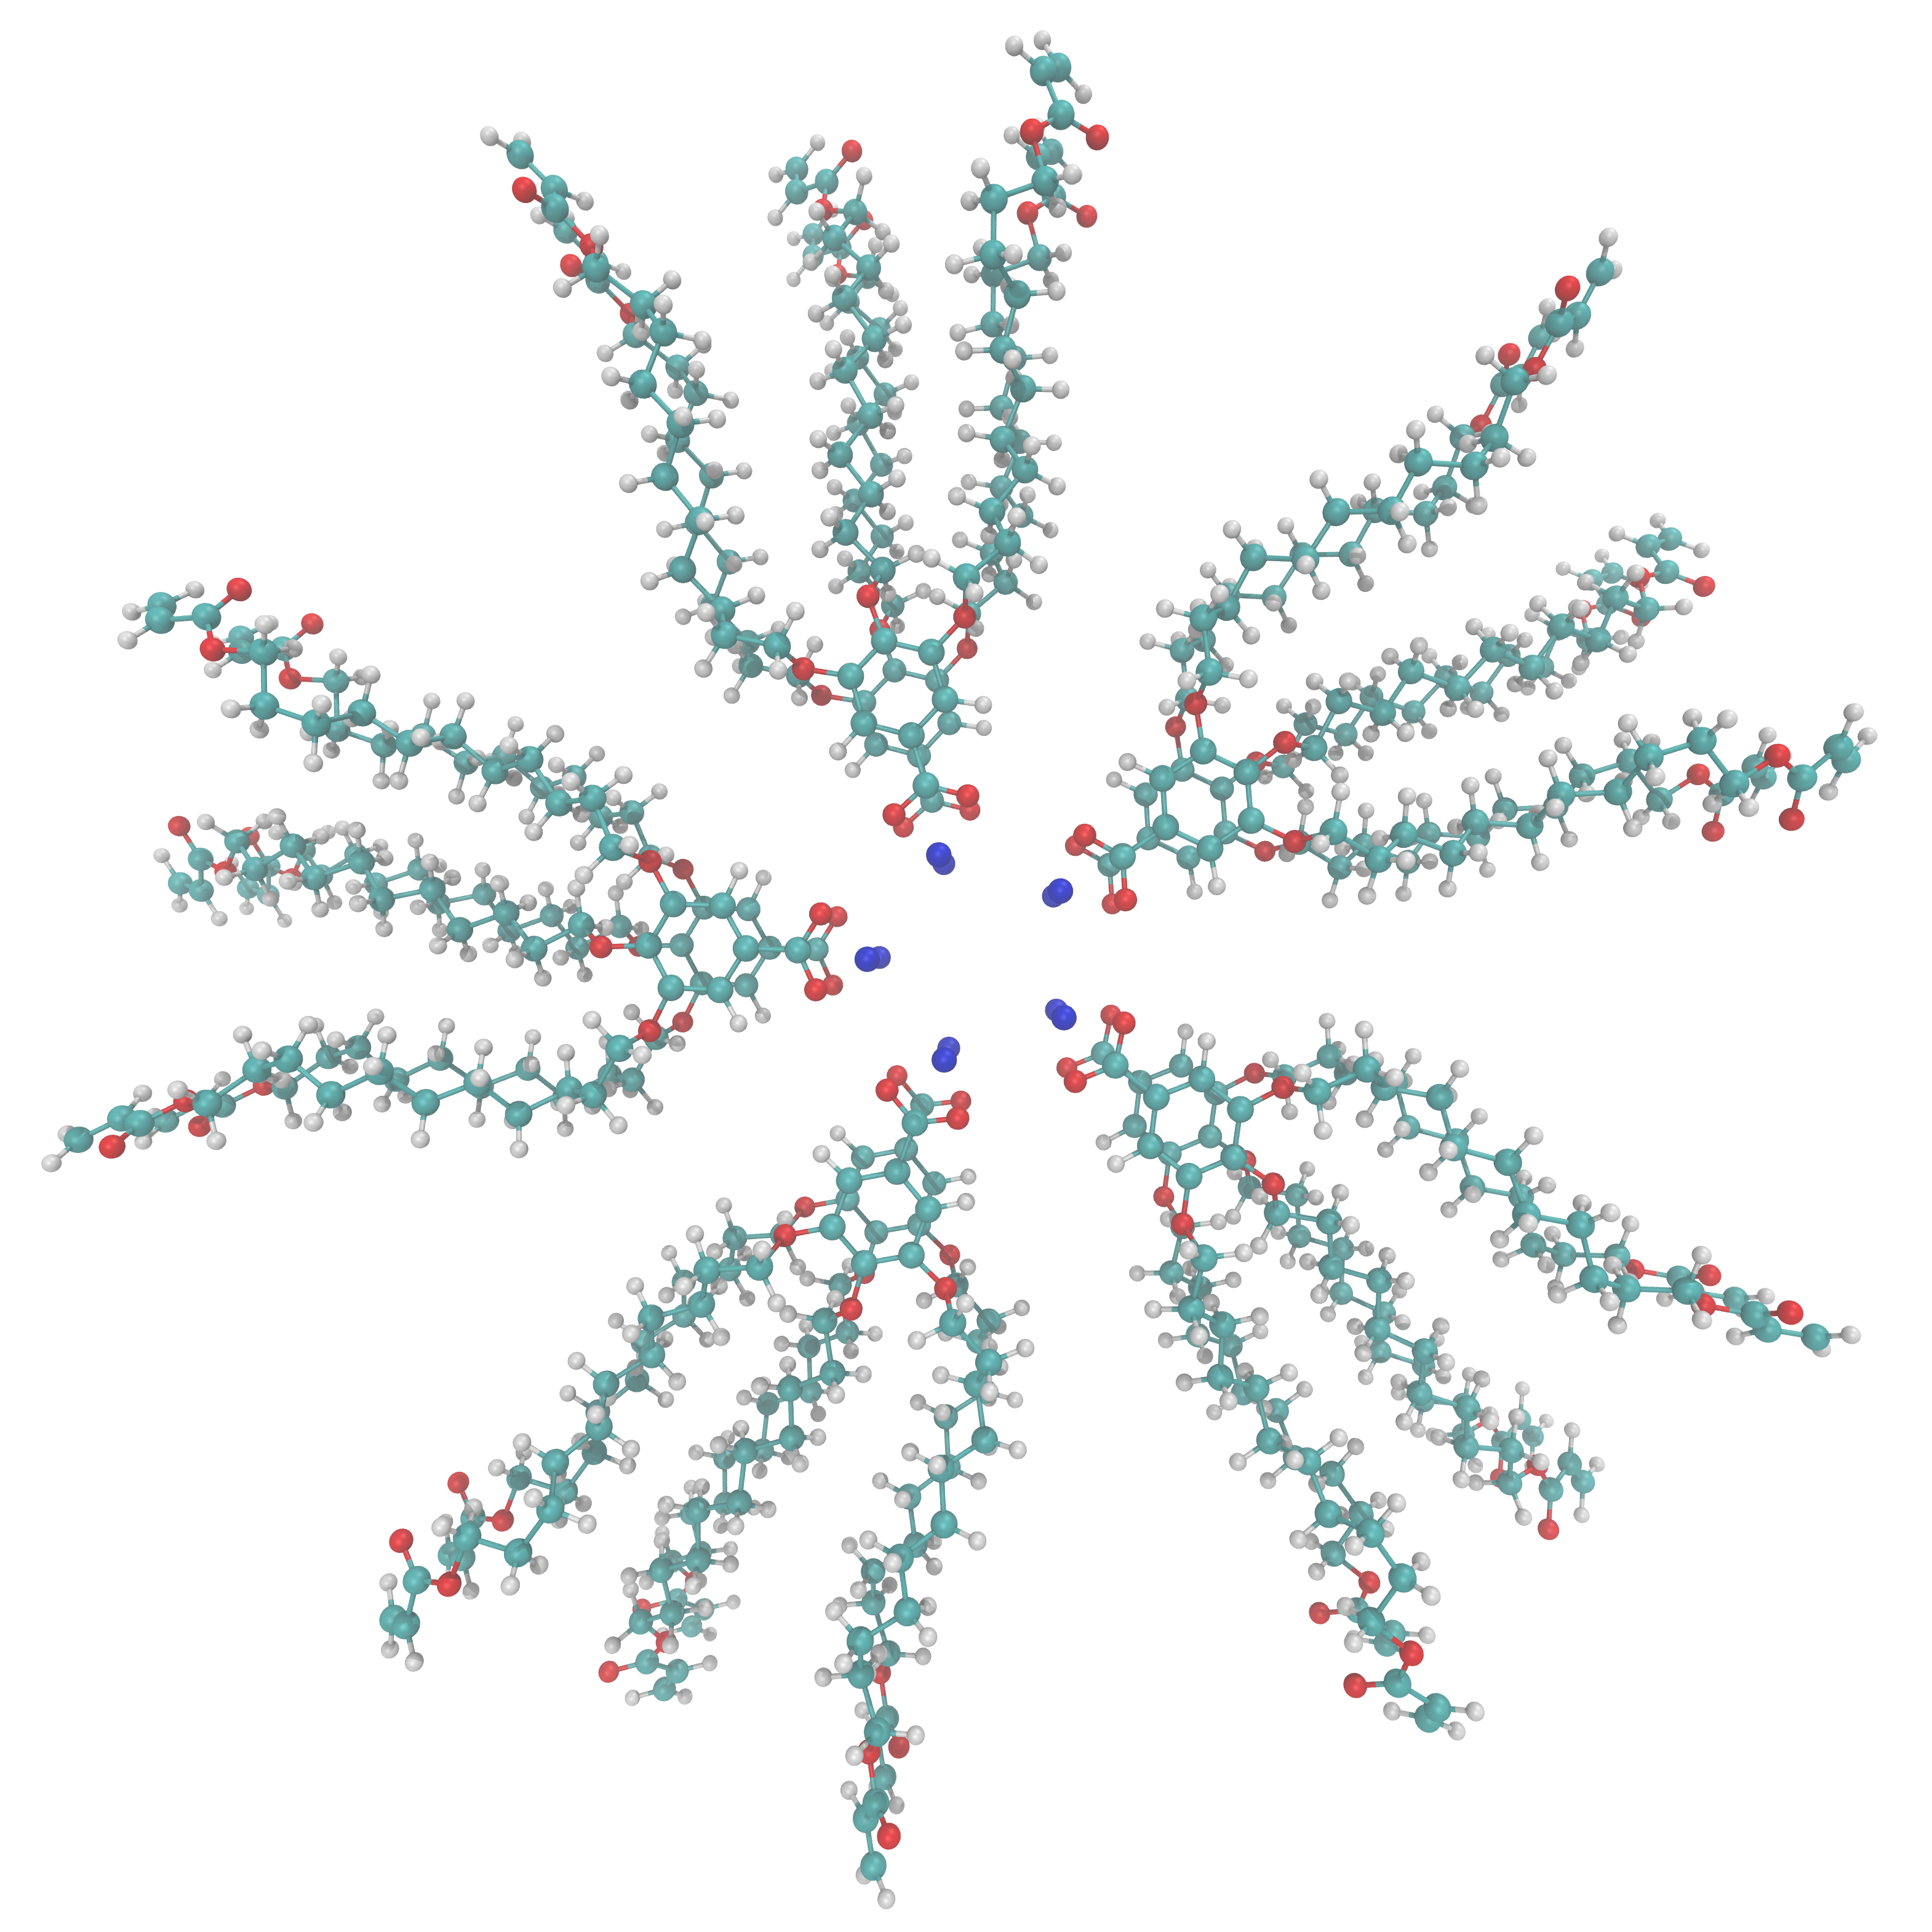
\includegraphics[width=\textwidth]{sandwichedlayers.png}
                \caption{}\label{fig:sandwichedlayers}
        \end{subfigure}
        \begin{subfigure}[b]{0.475\textwidth}
                \centering
                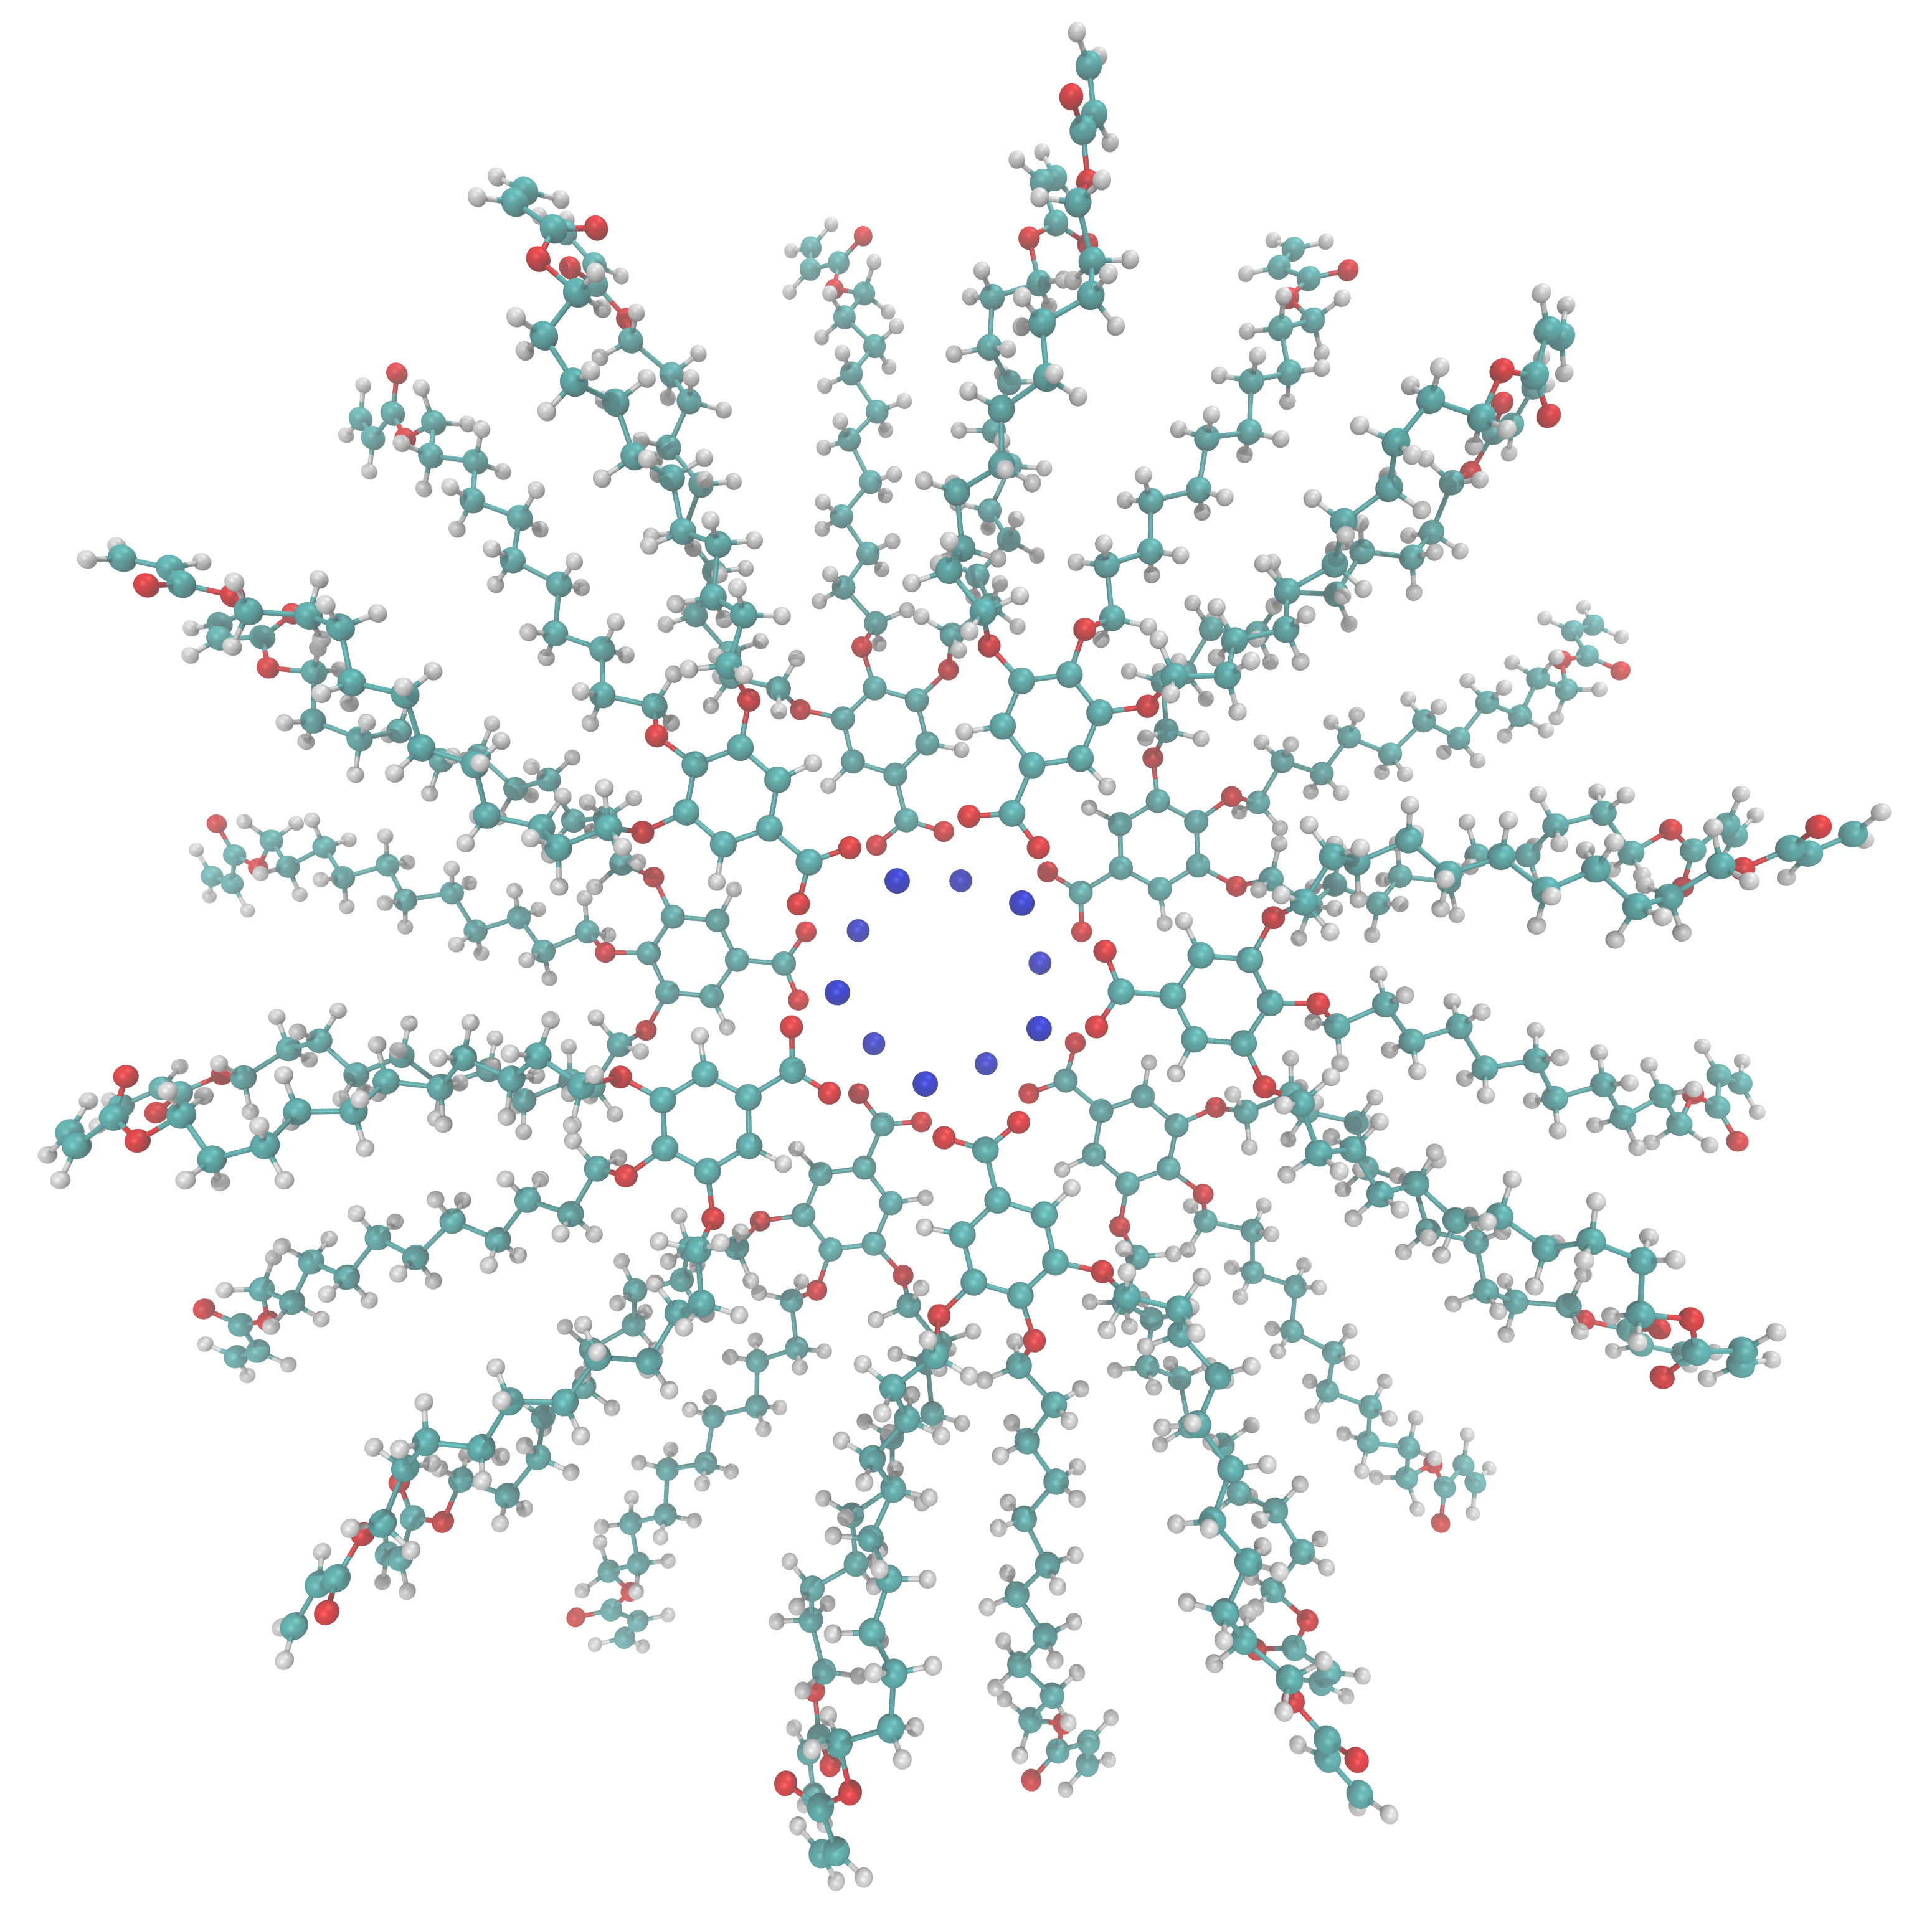
\includegraphics[width=\textwidth]{offsetlayers.png}
                \caption{}\label{fig:offsetlayers}
        \end{subfigure}
        \caption{(a) Sandwiched benzene dimers stack 3.8 \angstrom~apart. (b) Parallel-Displaced benzene dimers stack
        3.4 \angstrom~vertically and 1.6 \angstrom~horizontally apart. (c) T-shaped benzene dimers stack 5.0 \angstrom~apart.
        (d) Monomers stacked in the sandwiched configuration (e) Monomers stacked in the parallel-displaced
        configuration.}\label{fig:stacking}
  \end{figure}

  Based on evidence from section~\ref{M-section:rpi} of the main text, we
  believe it is most likely that the head groups stack somewhere between
  the sandwiched and parallel displaced modes which we studied (Figure~\ref{fig:between_pd}).

  \begin{figure}[!htb]
  \centering
  \begin{subfigure}{0.45\textwidth}
  \centering
  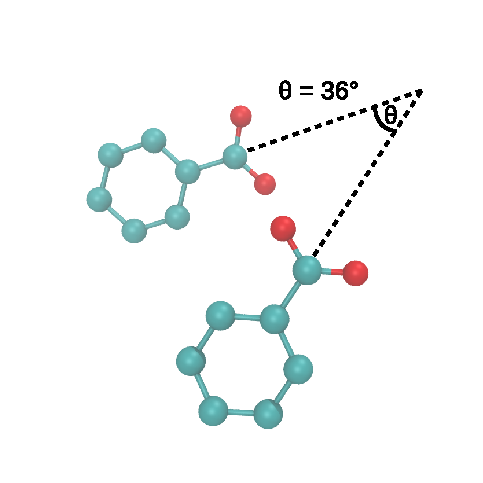
\includegraphics[width=\textwidth]{pd_36.eps}
  \caption{}\label{fig:pd_36}
  \end{subfigure}
  \begin{subfigure}{0.45\textwidth}
  \centering
  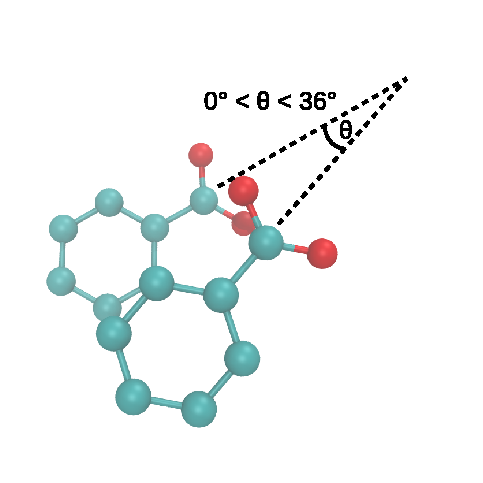
\includegraphics[width=\textwidth]{pd_lt36.eps}
  \caption{}\label{fig:pd_lt36}
  \end{subfigure}
  \caption{Head groups are likely stacked in a configuration between sandwiched and
  parallel displaced. (a) In our parallel displaced configurations with 5 columns 
  per pore, we placed head groups so the angle, $\theta$, between vectors extending
  from vertically stacked head groups to the pore center equals 36$\degree$ 
  ((360$\degree$ / $ncol$) / 2 , where $ncol$ is the number of columns per pore). 
  (b) In the true configuration, $\theta$ is likely distributed between 0$\degree$
  and 36 $\degree$. When $\theta$=0$\degree$, the system architecture is the same
  as a sandwiched configuration.}\label{fig:between_pd}
  \end{figure}

  \section{Equilibration Details}\label{section:equilibration}
  
  We developed equilibration schemes to create dry and wet configurations. Both
  schemes start with an initial configuration generated according to the previous
  guidelines. To create a dry configuration, we fix monomer head groups in the
  sandwiched or parallel-displaced configuration using position restraints with a
  force constant of 10$^6$ kJ mol$^{-1}$ nm$^{-2}$. We run a 50 ps simulation in
  the NVT ensemble which allows the monomer tails to settle without disrupting
  the ordering of the head groups. Doing so also mitigates system dependence on
  initial monomer configuration. Every 50 ps, we reduce the force constants by
  the square root of its previous value. Once the force constant is below 10 kJ
  mol$^{-1}$ nm$^{-2}$, we reduce the restraints in a sequence with values of
  8, 3, 2, 1, and 0 kJ mol$^{-1}$ nm$^{-2}$ respectively. We allow the resulting
  unrestrained structure to equilibrate for 5 ns in the NPT ensemble
  with pressure controlled by the Berendsen barostat. Next, we run long NPT
  equilibration simulations for at least 400 ns using the Parrinello-Rahman
  barostat with a time constant of 10 ps.

  % MRS6: some parameters missing here (time run between insertions, etc). 
  % I assume they are in supporting information?
  % BJC5: all water is present in initial configuration. This did not follow the more
  % complex procedures that I've come up with since then. 
  In order to create a ``wet'' system, we solvated an initial configuration with
  water using \texttt{gmx solvate}. We remove all water molecules placed outside
  the pore region. Then we randomly remove water molecules inside the pore region
  until the pores reach the desired concentration of water. The remainder of the
  equilibration follows the same procedure as the dry system. 

  \clearpage

  \section{Calculation of pore-to-pore spacing statistics}\label{section:p2p_stats}
 
 %BJC: is it really necessary to explain this if I release the code? I don't explain
 %any of the other stats I calculate. 
  We are interested in 5 pore-to-pore distances which should all be
  equal in a perfect hexagonal array (Figure~\ref{fig:p2p_diagram}). Only 4 of
  the 5 distances are independent. We can calculate a trajectory of spacing
  versus time for each of the 5 distances. We calculated the average pore-to-pore
  spacing and its uncertainty according to the following procedure:
   \begin{enumerate}
	\item We calculated the time when each of the pore-to-pore distances
	were equilibrated using \\ \texttt{pymbar.timeseries.detectEquilibration()}
	\cite{chodera_simple_2016,shirts_statistically_2008}. We began calculations
	after the largest of the five values.
	\item We calculated how long it takes for the data in each of the 5
	trajectories to become uncorrelated using \texttt{pymbar.timeseries.integratedAutocorrelationTime()}
	\cite{chodera_simple_2016,shirts_statistically_2008}. 
	\item We broke the full equilibrated trajectory into blocks of length $\tau$, where
	$\tau$ is the maximum of the five autocorrelation times calculated. Each block contains
	five sub-trajectories of pore-to-pore spacings.   
	\item We generate statistics using the bootstrapping technique. For
	each bootstrap trial, we reconstruct an equilibrium trajectory by randomly
	sampling from the trajectory blocks. 
	\item The average pore-to-pore distance is the mean of all pore
	spacings among all bootstrap trials.
	\item To calculate the uncertainty in pore-to-pore distance, we calculate the average 
	pore spacing for each pore over all bootstrap trials. Using the 5 average 
	pore-to-pore distances, we calculate the spread in a single pore-to-pore distance 
	with:
	\begin{equation}
	s = \sqrt{\frac{1}{4} \sum_{i=1}^5 (x_i - \overline{x})^2} 
	\label{equation:p2p_stats}
	\end{equation}
	where $\overline{x}$ is the average pore-to-pore distance. We divided the sum in 
	Equation~\ref{equation:p2p_stats} by 4 since there are only 4 independent pore
	spacings.
  \end{enumerate}
  
%BJC: included in a figure above
%  \begin{figure}[!htb]
%	\centering
%	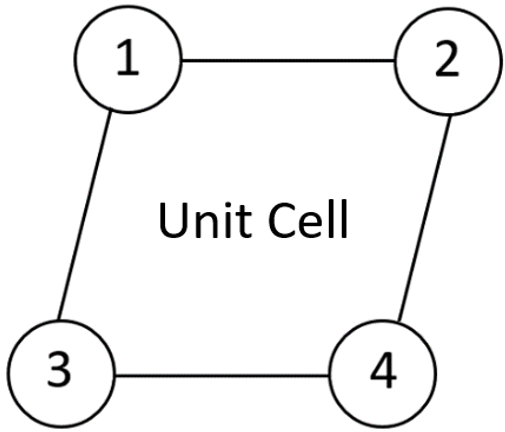
\includegraphics[width=0.25\textwidth]{p2p_diagram.png}
%	\caption{There are five pore-to-pore distances that are equal in a perfect
%		hexagon. If each number in the diagram represents the center of a
%		pore in a hexagonal unit cell, then the distance from 1 to 2, 2 to 4, 
%		4 to 3, 3 to 1 and 1 to 4 should be equal. Only 4 of the distances
%		are independent. For example, the distance from 1 to 4 is defined by
%		the location of all other pore centers.}
%	\label{fig:p2p_diagram}  
%  \end{figure}
  
  Alternatively, one can calculate the pore spacing as half of the $x$ and $y$
  box vectors, however this technique does not fully capture the uncertainty
  in the individual pore-to-pore distances (Table~\ref{table:p2p}). 
  
  \begin{table}[h]
  \centering
  \begin{tabular}{ccc}
  \toprule
  System                         & Pore Spacing ($nm$) & Pore Spacing ($nm$)              \\
                                 & Pore centers        & $\frac{1}{2}(x\ box\ vector)$ ($nm$) \\ 
  \midrule
  Sandwiched, Ordered            & 4.18 $\pm$ 0.13     & 4.16 $\pm$ 0.01                  \\
  Parallel Displaced, Ordered    & 4.17 $\pm$ 0.12     & 4.18 $\pm$ 0.01                  \\
  Sandwiched, Disordered         & 4.05 $\pm$ 0.14     & 4.01 $\pm$ 0.01                  \\
  Parallel Displaced, Disordered & 4.03 $\pm$ 0.07     & 4.01 $\pm$ 0.01                  \\
  \bottomrule
  \end{tabular}
  \caption{The pore spacing measured in two ways agree within uncertainty. In the main
  text, we report values calculated by measuring the average distance between pore centers. 
  Alternatively, one can estimate the pore spacing as half of the $x$ and $y$ box vectors.
  Both methods agree within uncertainty, but measuring the distance between pore centers
  does a better job of showing the spread of pore-to-pore distances.}~\label{table:p2p}
  \end{table}

  \clearpage

  \section{2D Small Angle X-ray Scattering Data}  
 
  \begin{figure}[!htb]
  \centering
  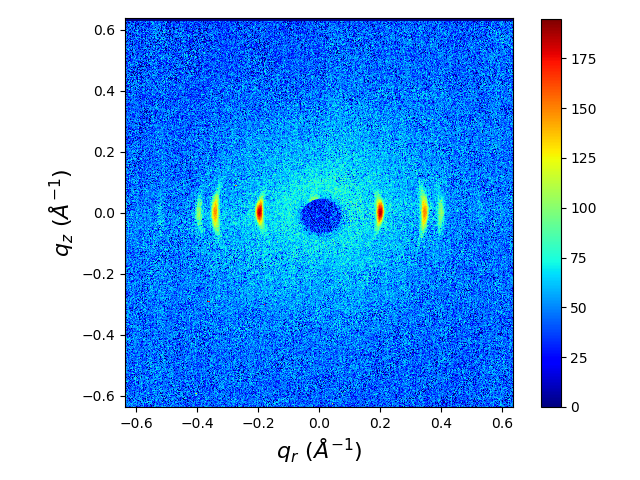
\includegraphics[width=0.5\textwidth]{2DSAXS_axes.png}
  \caption{Two dimensional small angle X-ray scattering experiments show
  reflections along the $q_r$ axis at $q_z$=0. The spacing between the reflections
  is characteristic of a hexagonal phase and is directly related to the distance
  between pores. The reflections are arced because the pores are not perfectly
  aligned. A perfectly aligned system would show dots at each peak location. An
  isotropically aligned system would show concentric rings about the origin which
  pass through each peak location. The d\textsubscript{100} and d\textsubscript{110} 
  peaks (the first two pairs of reflections from origin located at $|\mathbf{q}| 
  \approx 0.18~\AA^{-1}$ and $|\mathbf{q}| \approx 0.31~\AA^{-1}$) are not visible
  in the 2D WAXS pattern. The edges of the d\textsubscript{200} reflection (the third
  pair of reflections located at $|\mathbf{q}| \approx 0.36~\AA^{-1}$) are slightly
  visible in the 2D WAXS pattern, so we used them to approximate the experimental
  intensity of R-pores.}\label{fig:2DSAXS}
  \end{figure}

  \newpage

  \section{Component radial density functions}\label{section:radial_density}
 %BJC: can probably delete this figure 
  \begin{figure}[!htb]
  \centering
  \begin{subfigure}{0.47\textwidth}
        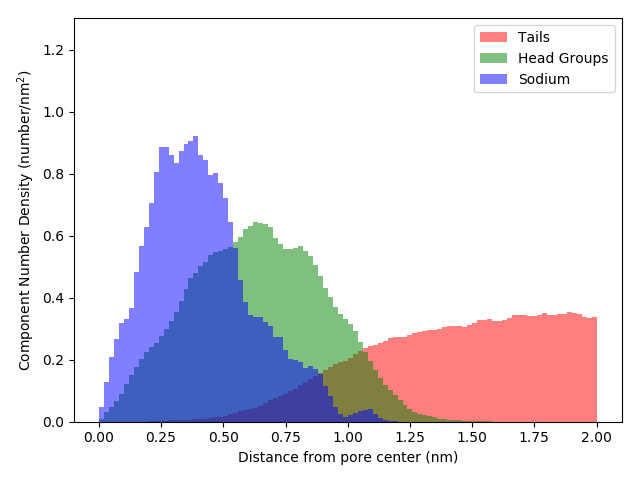
\includegraphics[width=1\linewidth]{offset_density.png}
        \caption{Parallel Displaced, Ordered Pore Basin}
        \label{fig:offset_density}
  \end{subfigure}
  \begin{subfigure}{0.47\textwidth}
        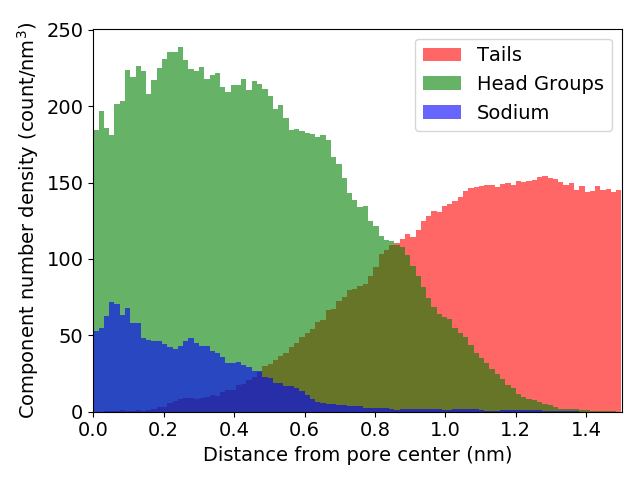
\includegraphics[width=1\linewidth]{layered_density.png}
        \caption{Sandwiched, Ordered Pore Basin}
        \label{fig:layered_density}
  \end{subfigure}
  \begin{subfigure}{0.47\textwidth}
        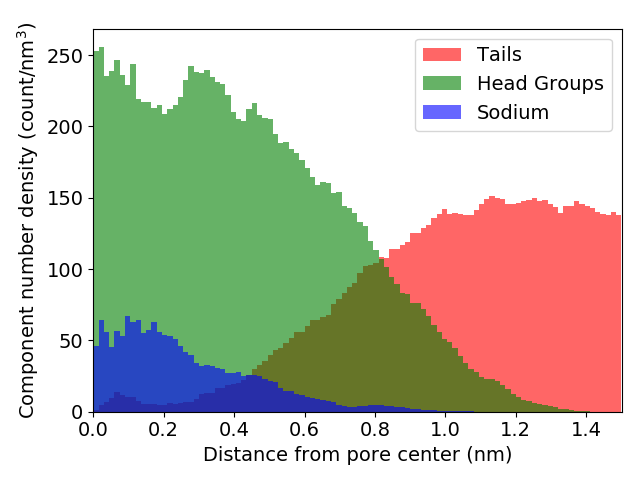
\includegraphics[width=1\linewidth]{disordered_offset_density.png}
        \caption{Parallel Displaced, Disordered Pore Basin}
        \label{fig:disordered_offset_density}
  \end{subfigure}
  \begin{subfigure}{0.47\textwidth}
        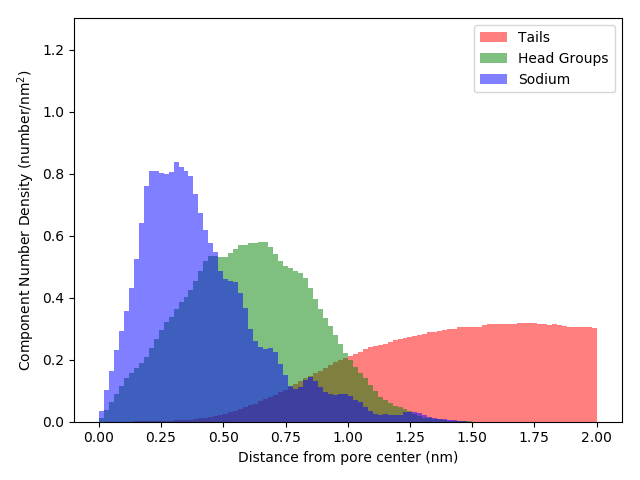
\includegraphics[width=1\linewidth]{disordered_density.png}
        \caption{Sandwiched, Disordered Pore Basin}
        \label{fig:disorder_layered_density}
  \end{subfigure}
  %MRS8: at least one of these would be good to put in the main paper.
  \caption{In all cases, the component radial distribution functions exhibit a
	  composition gradient transitioning from the hydrophilic to the hydrophobic
	  regions. Systems with monomers initially stacked 3.7 \AA~apart in the parallel
	  displaced (a), and sandwiched (b) configurations both show the highest
	  concentrations of ions and head groups away from the pore center. Systems with
	  layers initially spaced 5 \AA~apart (c) and (d), both show the highest
	  concentrations of ions and head groups near the pore center, implying a more
	  uniform, disordered pore.}~\label{fig:densities}
  \end{figure}
  \clearpage

  \begin{figure}
  \begin{minipage}{0.45\linewidth}
  \centering
  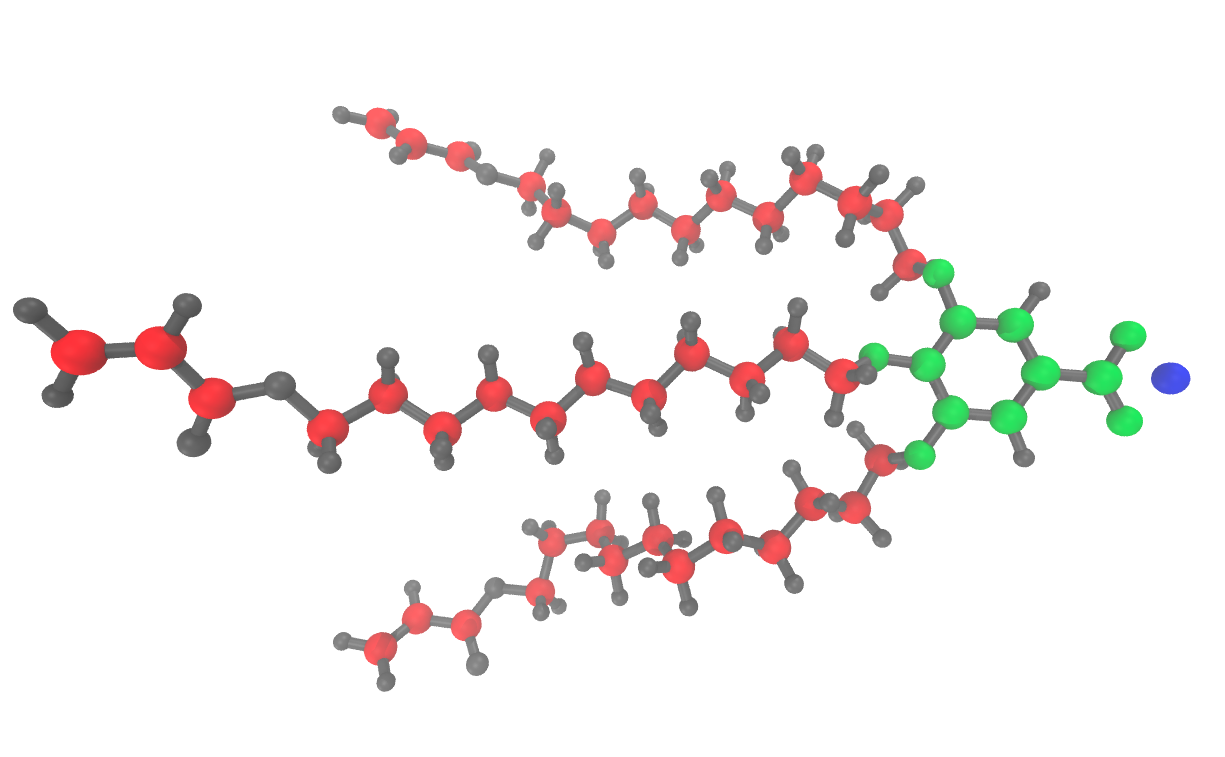
\includegraphics[width=\textwidth]{monomer_color_coded.png}
  \vspace{4.5em}
  \caption{The groups used for radial distribution calculations. Red atoms are in the
  tails group. Green atoms are in the head group region. The blue atom is sodium.}\label{fig:monomer_color_coded}
  \end{minipage}\qquad
  \begin{minipage}{0.45\textwidth}
  \centering
  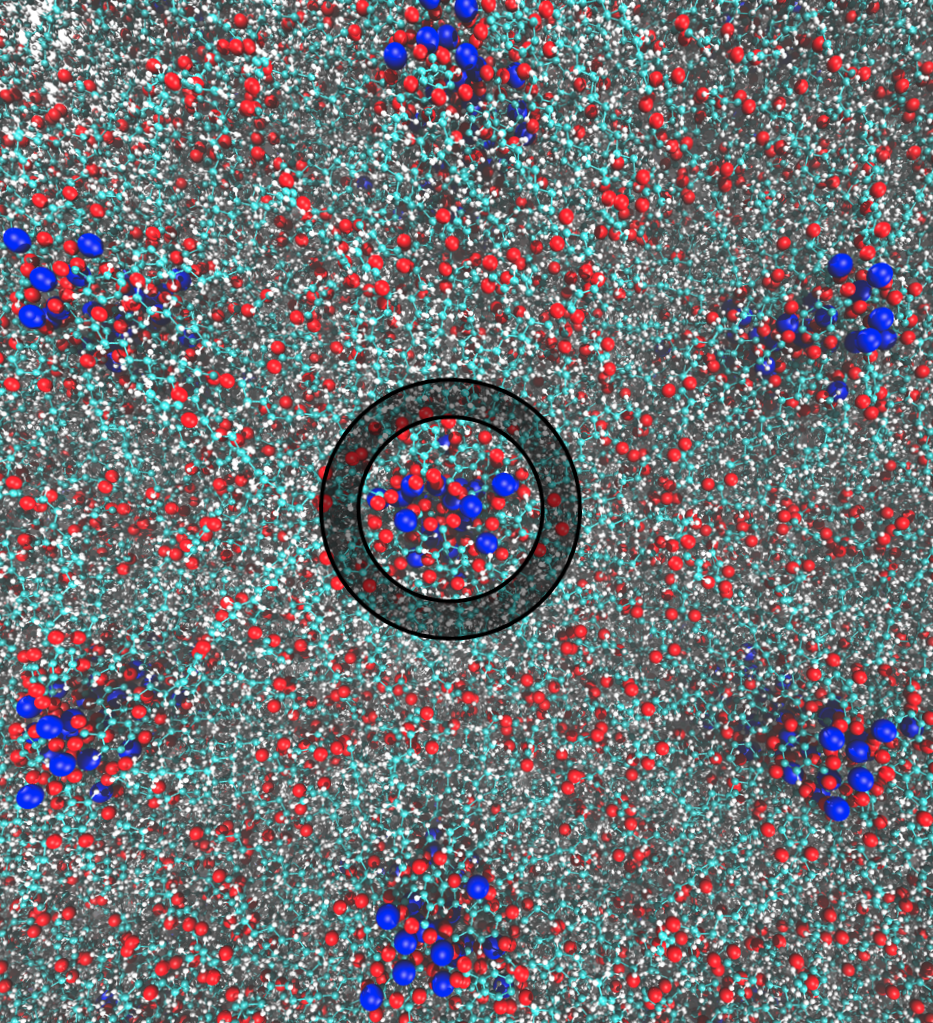
\includegraphics[width=\linewidth]{radial_distribution_annulus.png}
  \caption{
  Looking down onto the $xy$ plane of the membrane, 
  % this diagram
  % illustrates how we calculated radial distribution
  % functions.
  we binned the radial distance of all atoms in chosen groups from
  pore centers. The bins are defined by the annulus bounded by concentric
  circles centered at the pore centers, as shown. We normalize by
  dividing the count of atoms within each bin annulus by its volume.
%  of
%  the annulus where the volume is the area of the annulus times the
%  height of the membrane in the z-direction.
  }~\label{fig:rdf_diagram}
  \end{minipage}
  \end{figure}
% BJC: Unnecessary, supporting info already long
%  \begin{figure}
%	\centering
%        \begin{subfigure}{0.40\textwidth}
%                \centering
%                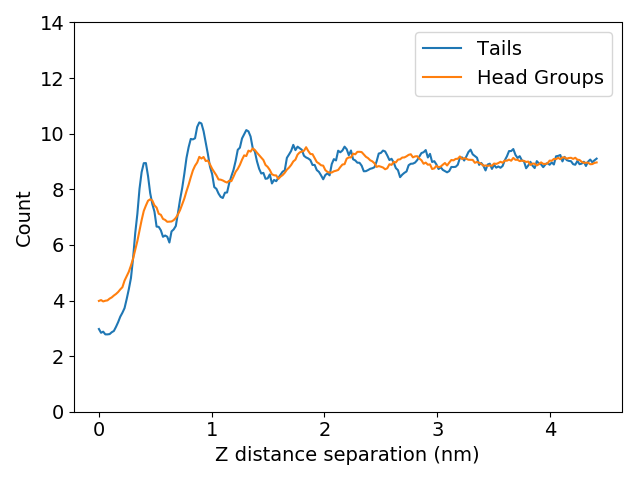
\includegraphics[width=\textwidth]{zdf_layered_4.png}
%                \caption{4 mon/layer, Sandwiched}\label{fig:zdf_layered_4}
%        \end{subfigure}
%        \begin{subfigure}{0.40\textwidth}
%                \centering
%                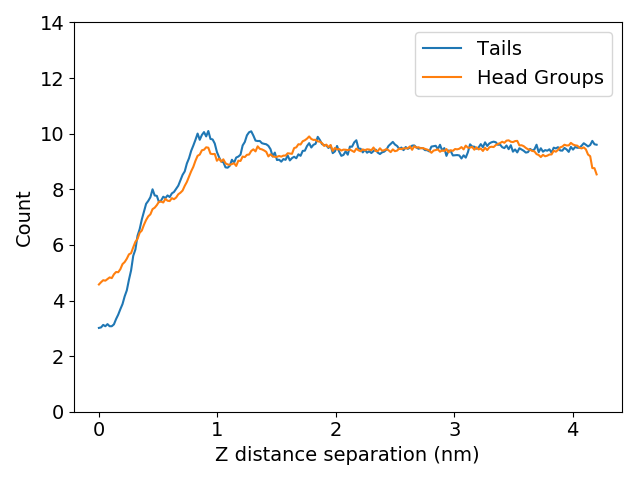
\includegraphics[width=\textwidth]{zdf_offset_4.png}
%                \caption{4 mon/layer, Parallel Displaced}\label{fig:zdf_layered_4}
%        \end{subfigure}
%	\begin{subfigure}{0.40\textwidth}
%                \centering
%                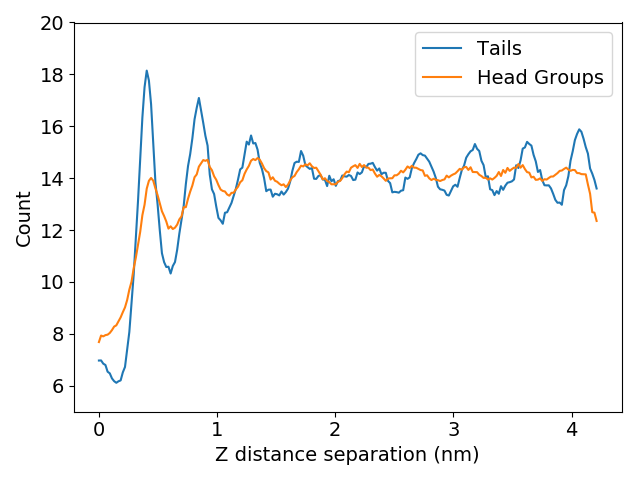
\includegraphics[width=\textwidth]{zdf_layered_6.png}
%                \caption{6 mon/layer, Sandwiched}\label{fig:zdf_layered_6}
%        \end{subfigure}
%        \begin{subfigure}{0.40\textwidth}
%                \centering
%                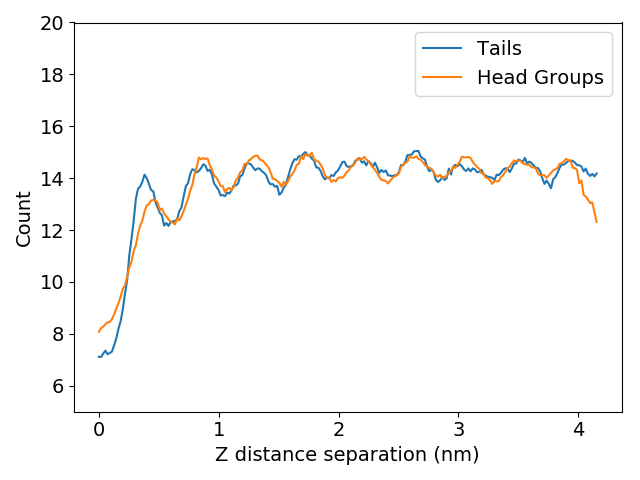
\includegraphics[width=\textwidth]{zdf_offset_6.png}
%                \caption{6 mon/layer, Parallel Displaced}\label{fig:zdf_layered_6}
%        \end{subfigure}
%        \begin{subfigure}{0.40\textwidth}
%                \centering
%                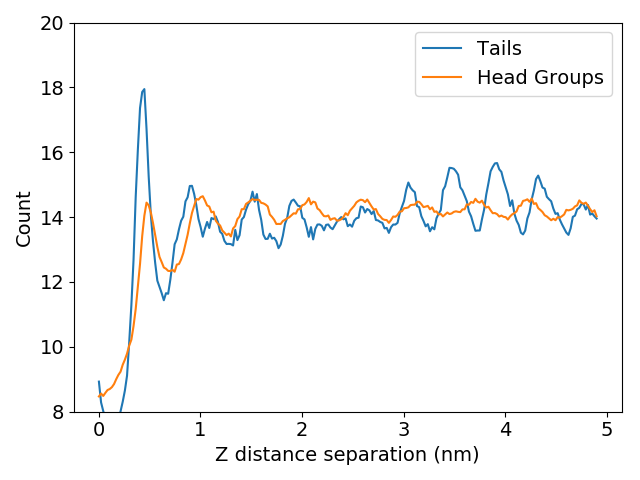
\includegraphics[width=\textwidth]{zdf_layered_7.png}
%                \caption{7 mon/layer, Sandwiched}\label{fig:zdf_layered_7}
%        \end{subfigure}
%        \begin{subfigure}{0.40\textwidth}
%                \centering
%                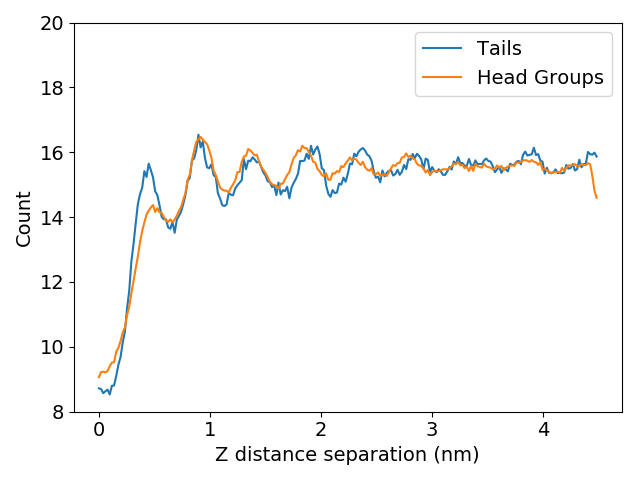
\includegraphics[width=\textwidth]{zdf_offset_7.png}
%                \caption{7 mon/layer, Parallel Displaced}\label{fig:zdf_layered_7}
%        \end{subfigure}
%	\begin{subfigure}{0.40\textwidth}
%                \centering
%                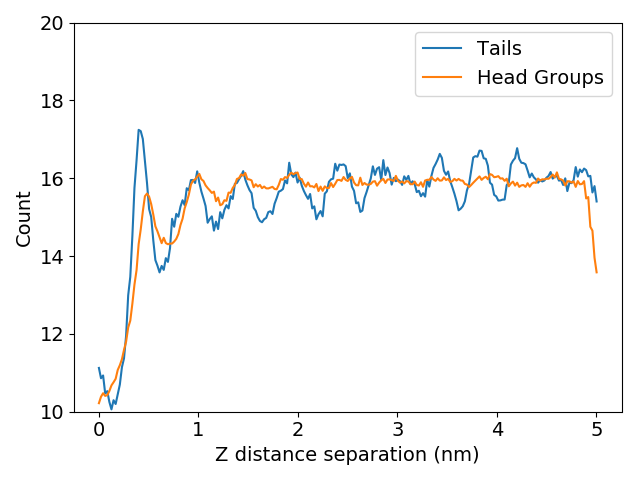
\includegraphics[width=\textwidth]{zdf_layered_8.png}
%                \caption{8 mon/layer, Sandwiched}\label{fig:zdf_layered_8}
%        \end{subfigure}
%        \begin{subfigure}{0.40\textwidth}
%                \centering
%                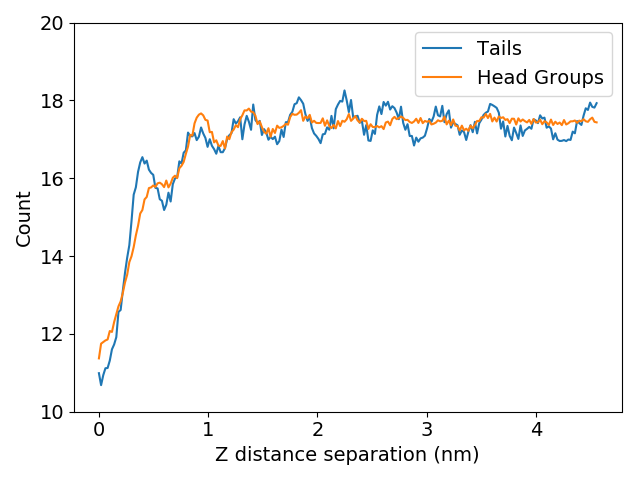
\includegraphics[width=\textwidth]{zdf_offset_8.png}
%                \caption{8 mon/layer, Parallel Displaced}\label{fig:zdf_layered_8}
%        \end{subfigure}
%	\caption{$g(z)$ for all other configurations built with layers stacked 3.7 \AA~apart}\label{fig:zdf}
%  \end{figure}

%BJC: unnecessary. Supporting info already long..and more is coming
%  \begin{figure}
%	\centering
%        \begin{subfigure}{0.40\textwidth}
%                \centering
%                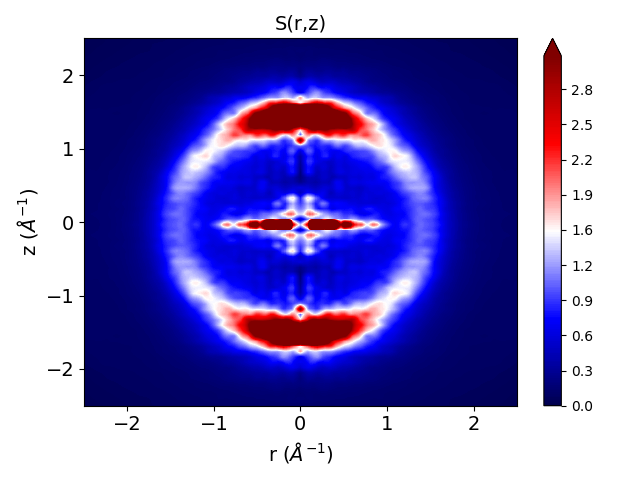
\includegraphics[width=\textwidth]{rzplot_layered_4.png}
%                \caption{4 mon/layer, Sandwiched}\label{fig:rzplot_layered_4}
%        \end{subfigure}
%        \begin{subfigure}{0.40\textwidth}
%                \centering
%                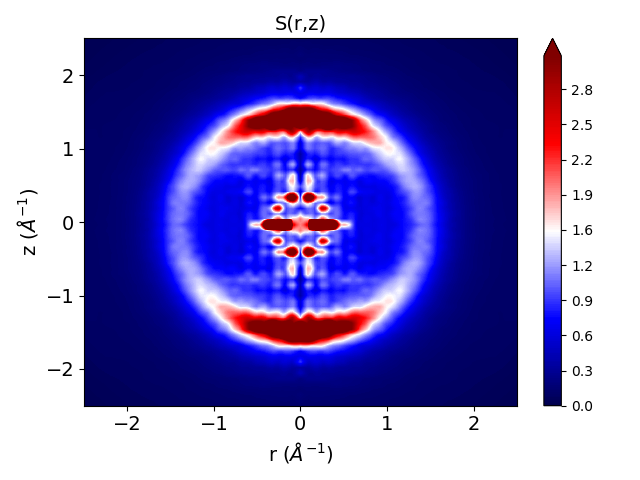
\includegraphics[width=\textwidth]{rzplot_offset_4.png}
%                \caption{4 mon/layer, Parallel Displaced}\label{fig:rzplot_offset_4}
%        \end{subfigure}
%        \begin{subfigure}{0.40\textwidth}
%                \centering
%                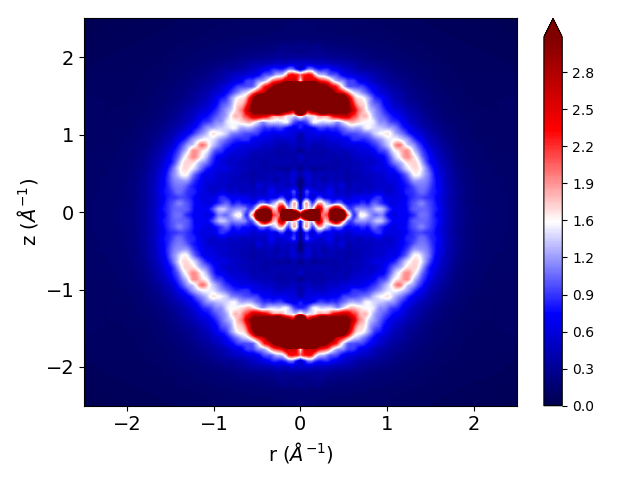
\includegraphics[width=\textwidth]{rzplot_layered_6.png}
%                \caption{6 mon/layer, Sandwiched}\label{fig:rzplot_layered_6}
%        \end{subfigure}
%        \begin{subfigure}{0.40\textwidth}
%                \centering
%                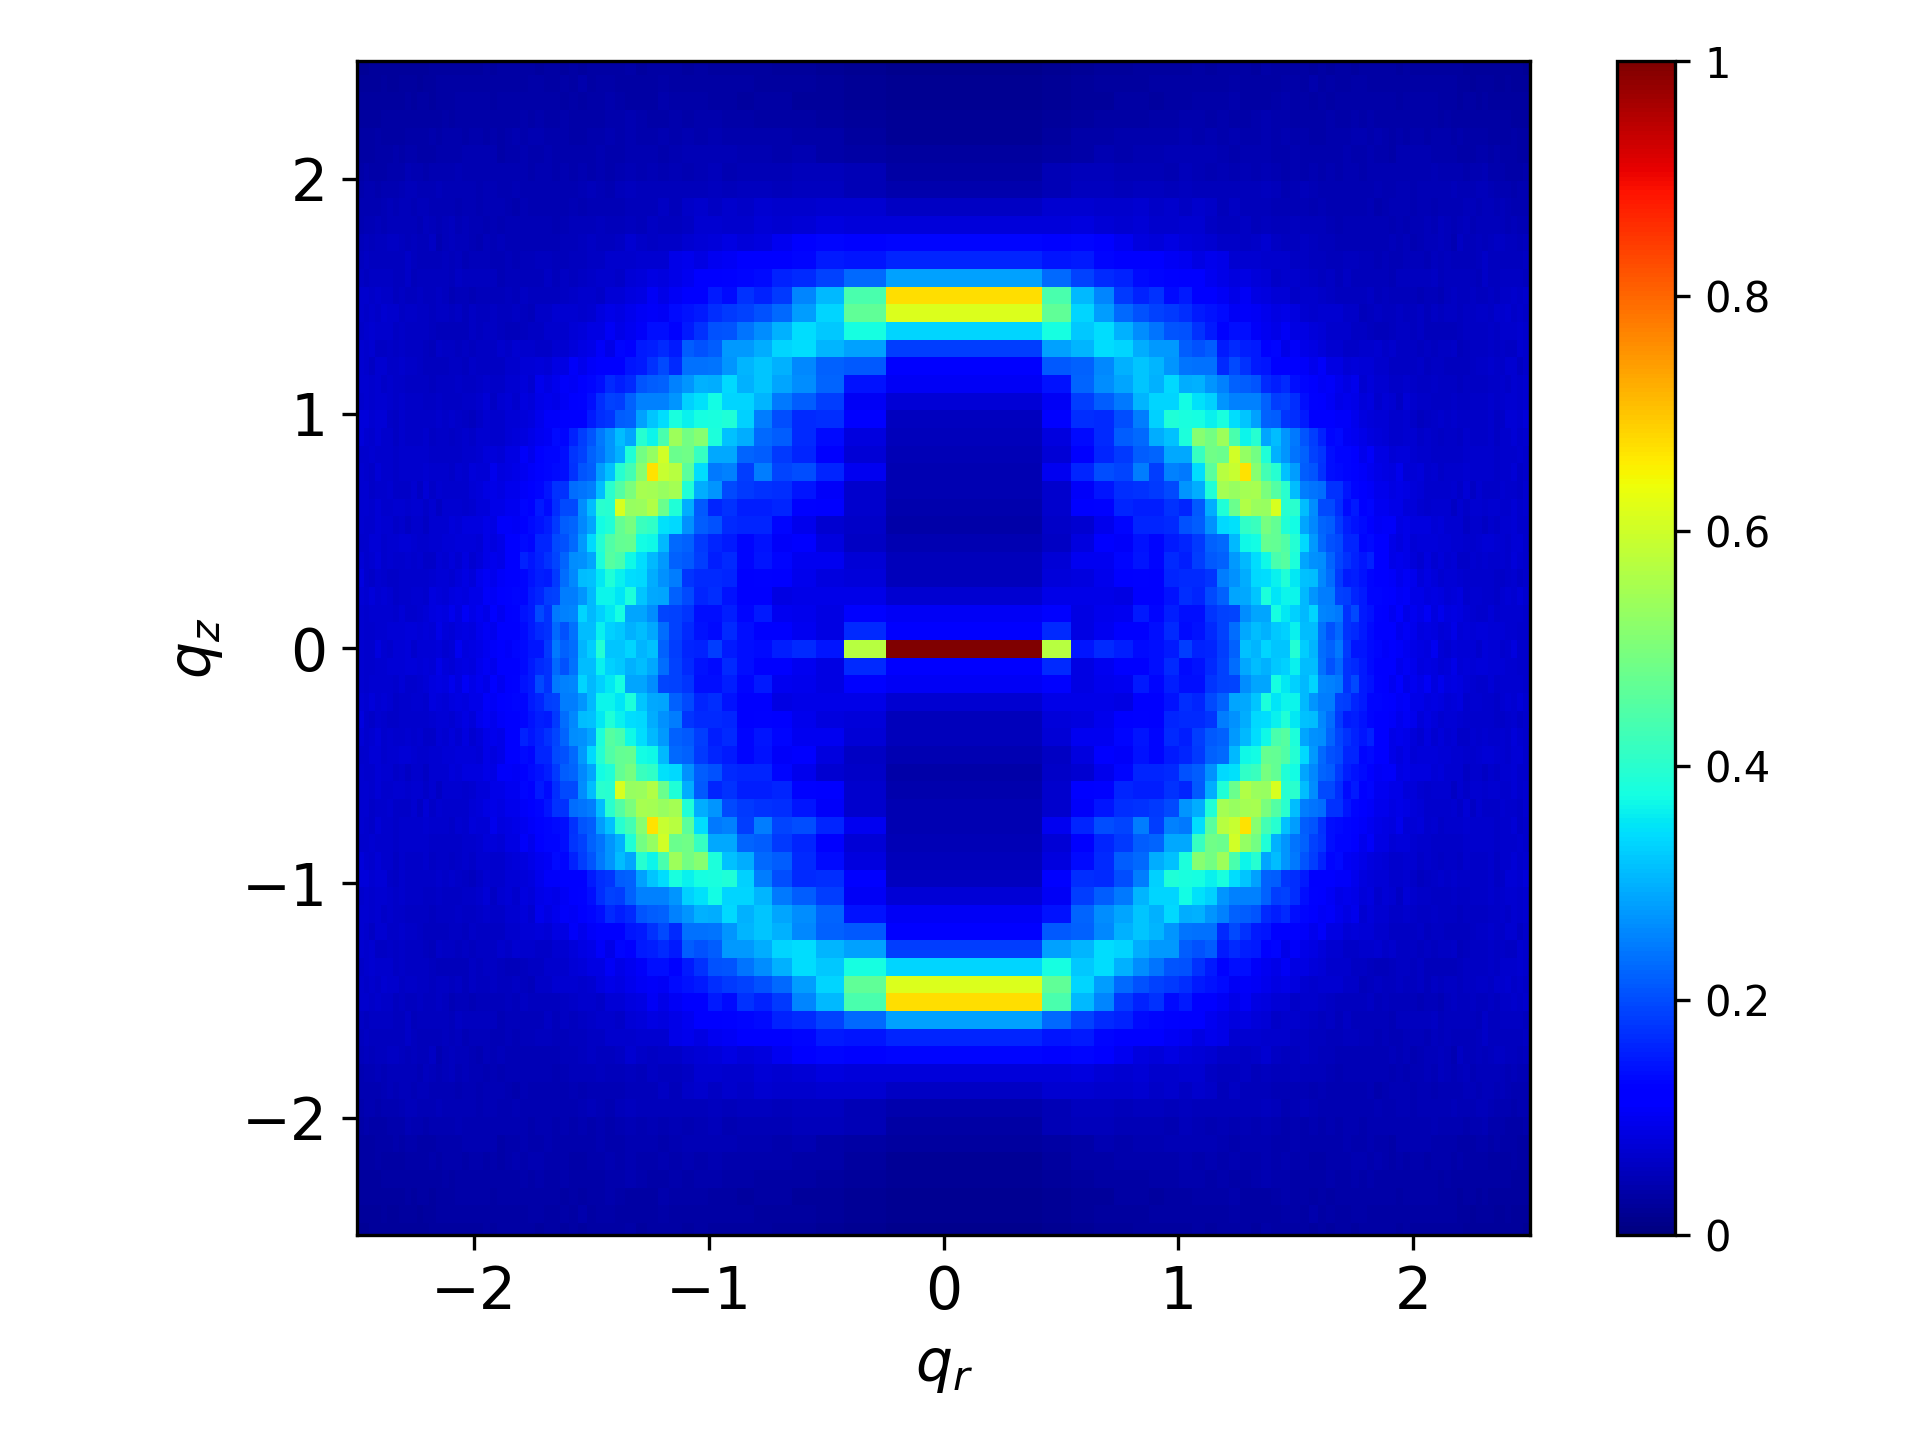
\includegraphics[width=\textwidth]{rzplot_offset_6.png}
%                \caption{6 mon/layer, Parallel Displaced}\label{fig:rzplot_offset_6}
%        \end{subfigure}
%        \begin{subfigure}{0.40\textwidth}
%                \centering
%                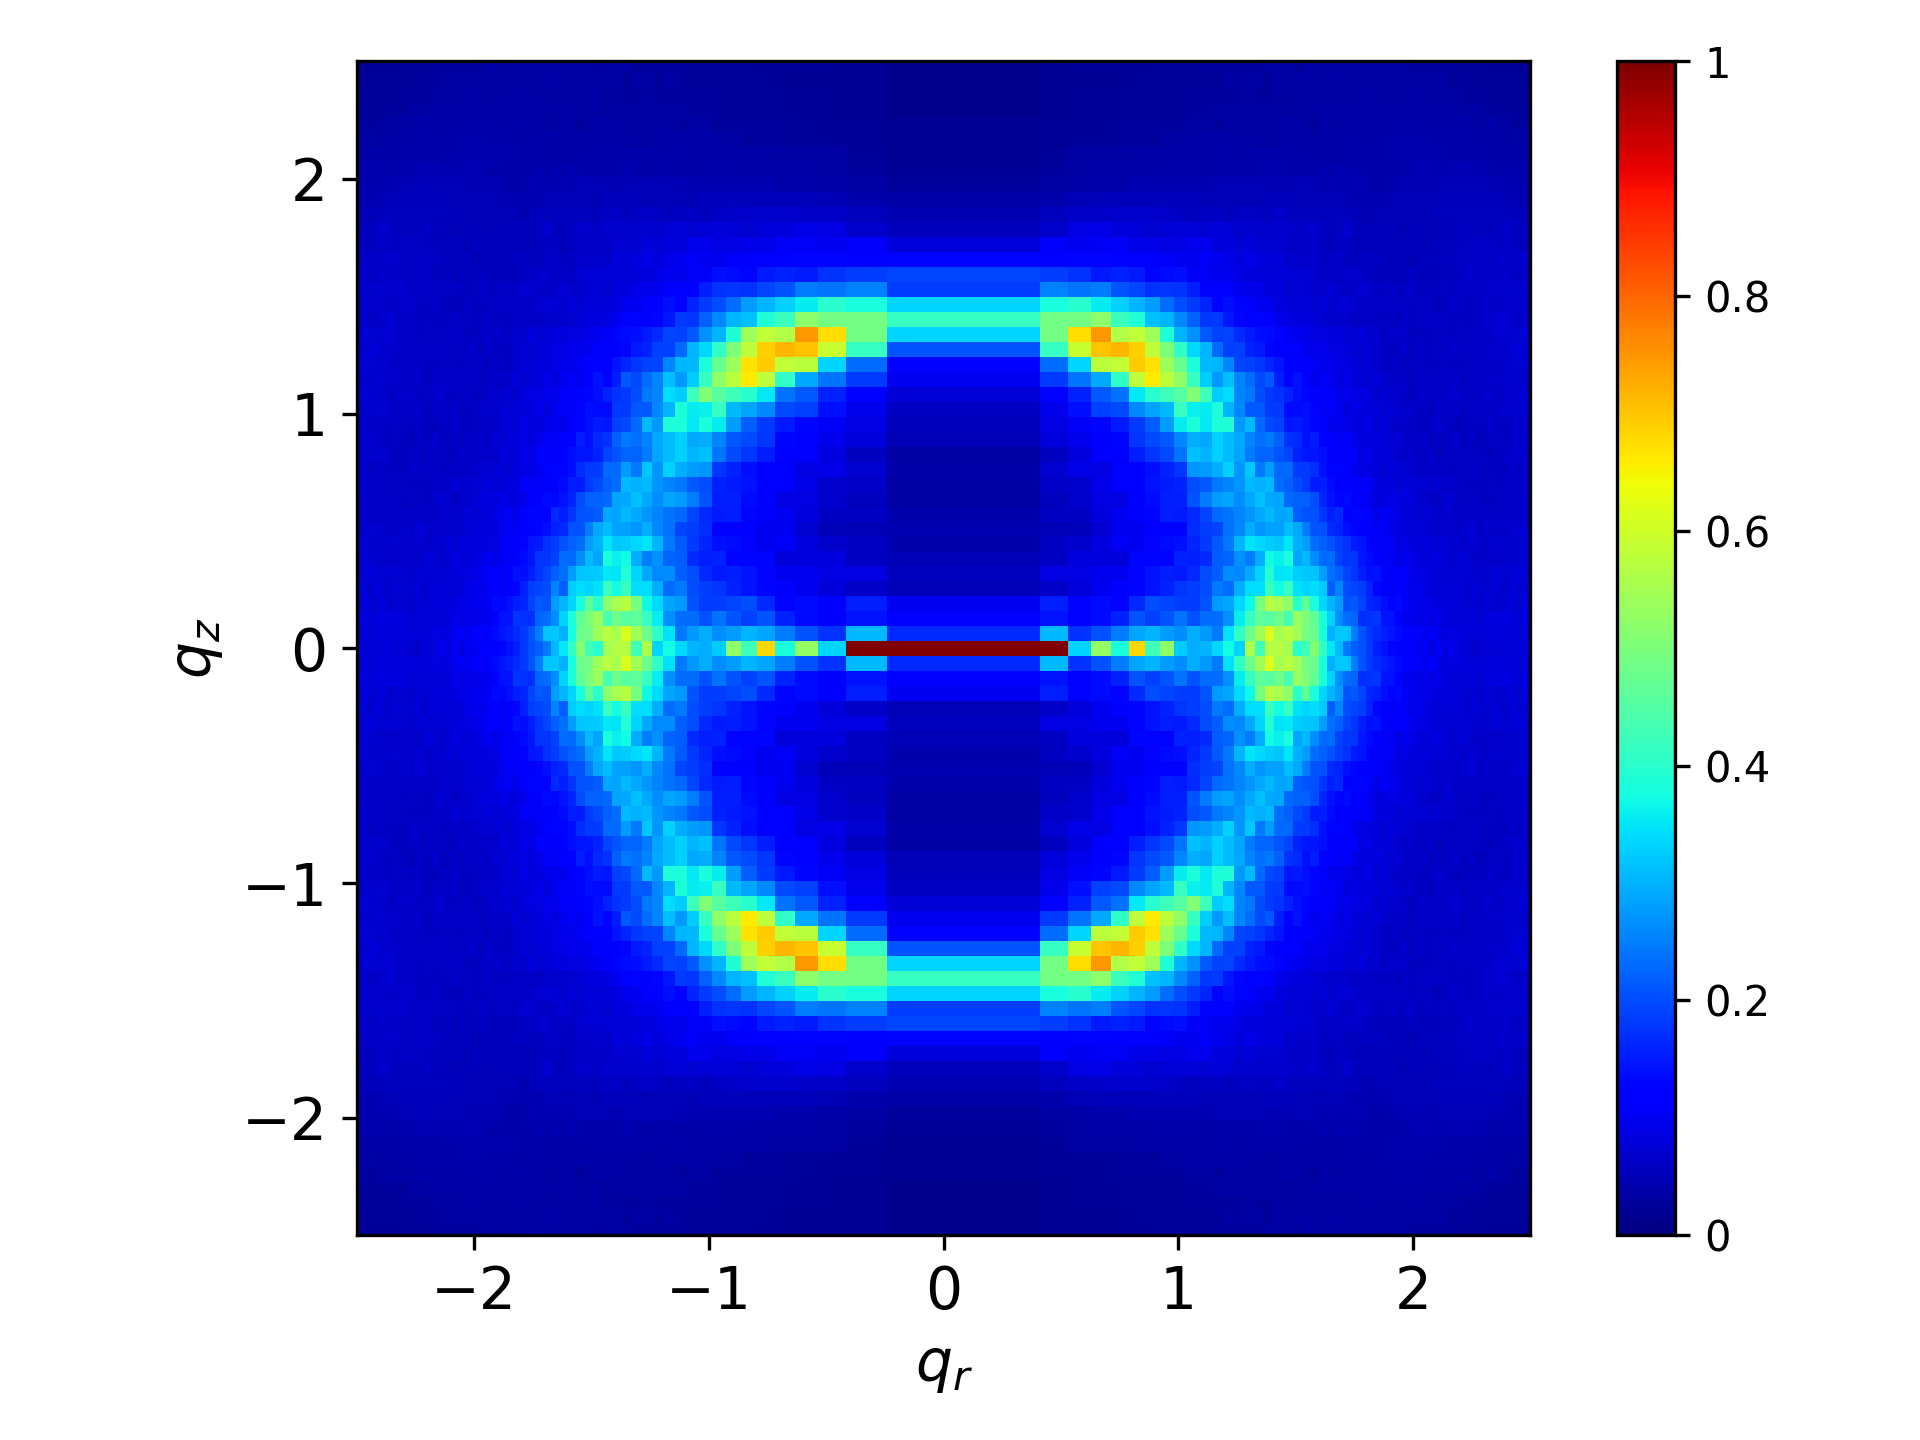
\includegraphics[width=\textwidth]{rzplot_layered_7.png}
%                \caption{7 mon/layer, Sandwiched}\label{fig:rzplot_layered_7}
%        \end{subfigure}
%        \begin{subfigure}{0.40\textwidth}
%                \centering
%                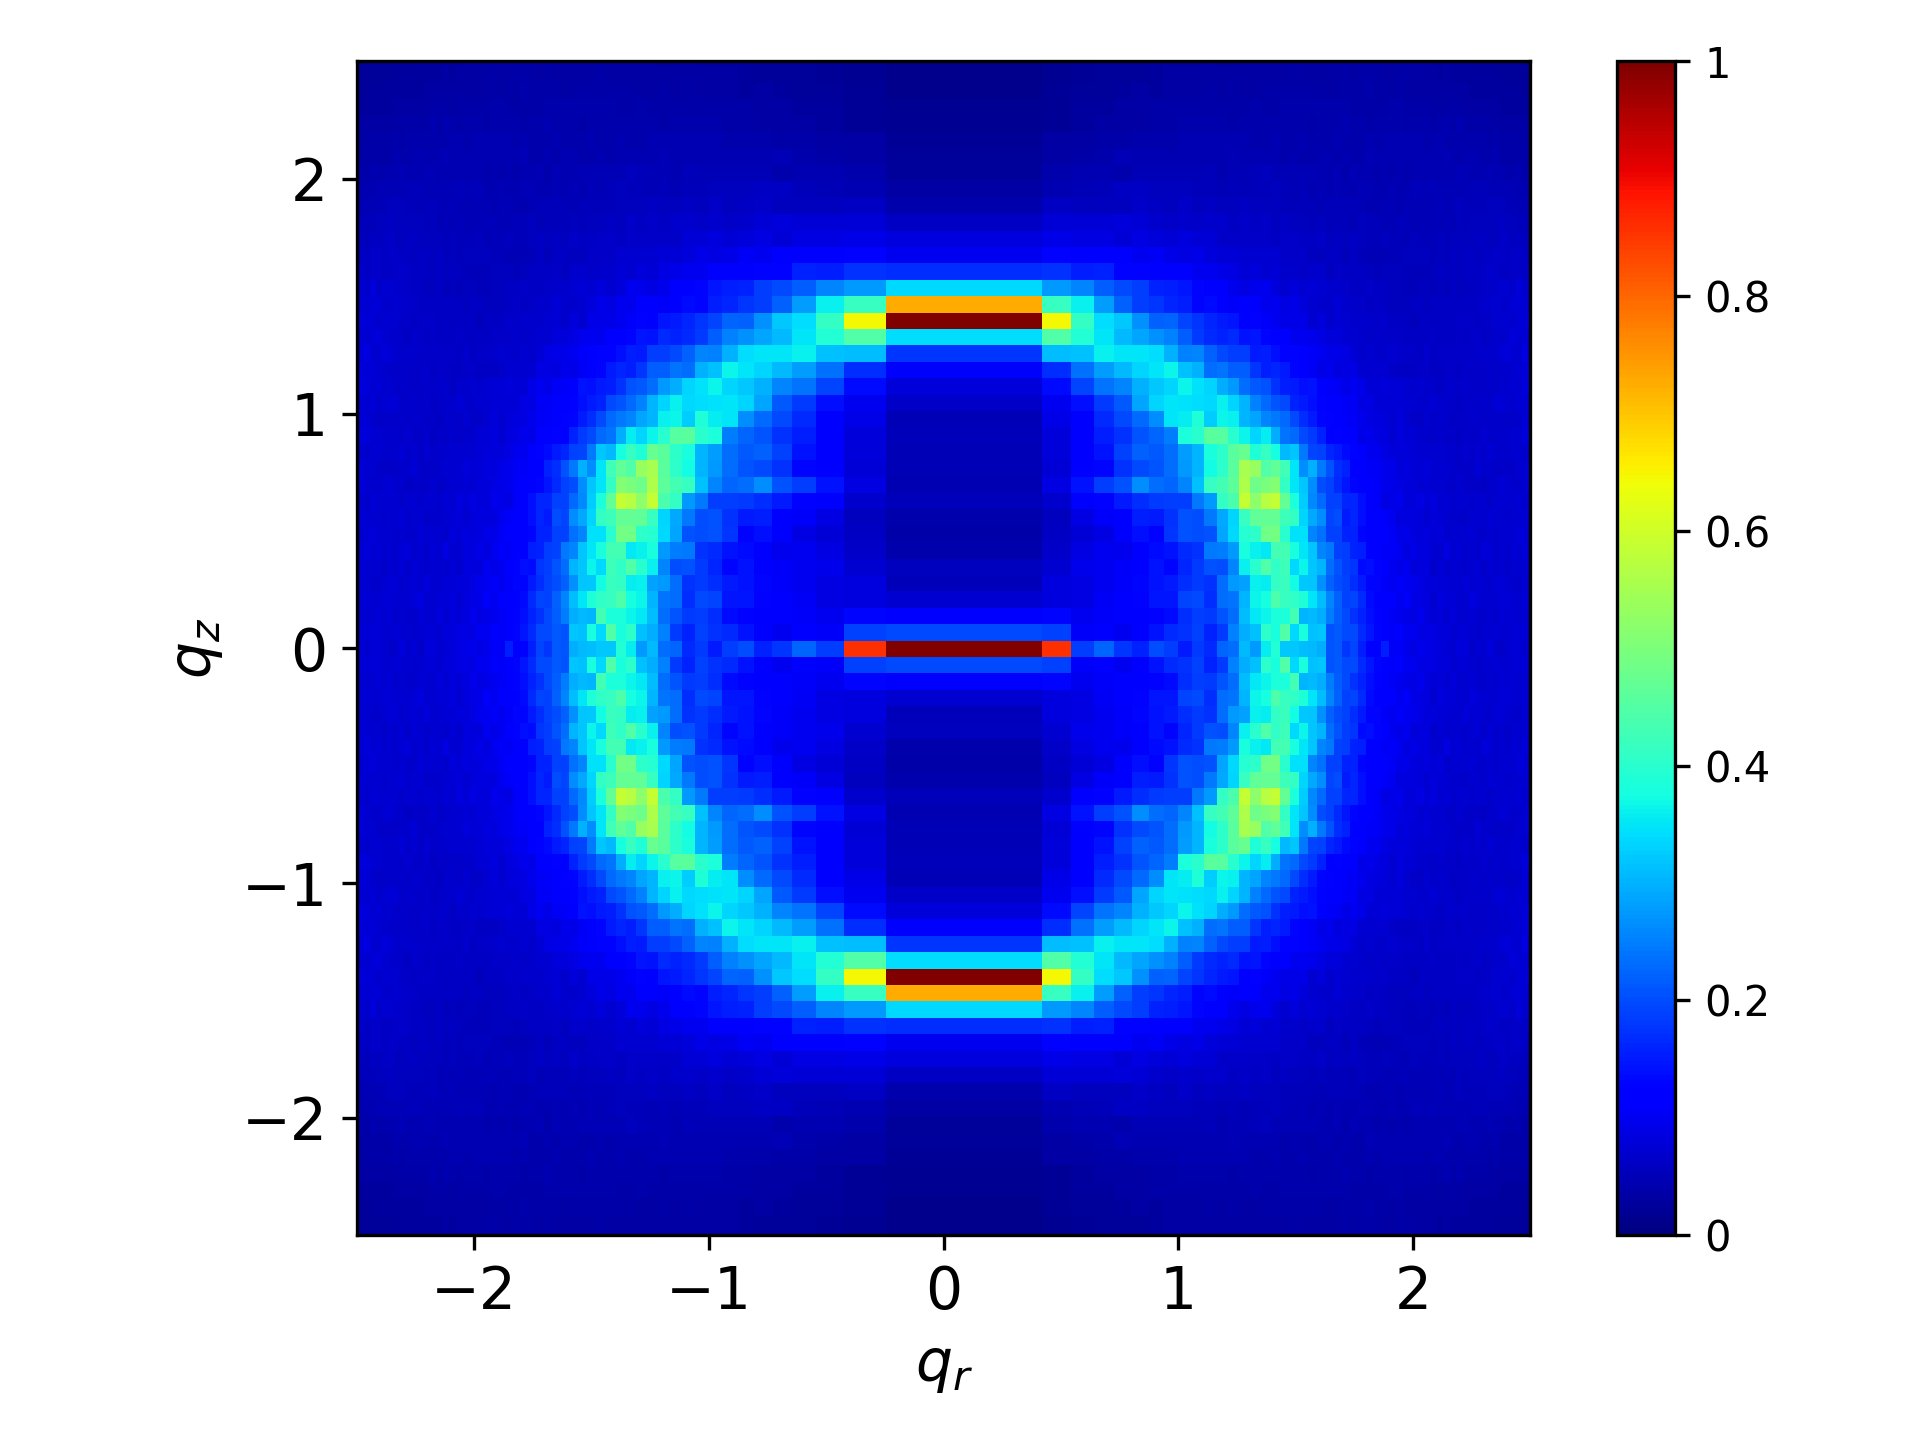
\includegraphics[width=\textwidth]{rzplot_offset_7.png}
%                \caption{7 mon/layer, Parallel Displaced}\label{fig:rzplot_offset_7}
%        \end{subfigure}
%        \begin{subfigure}{0.40\textwidth}
%                \centering
%                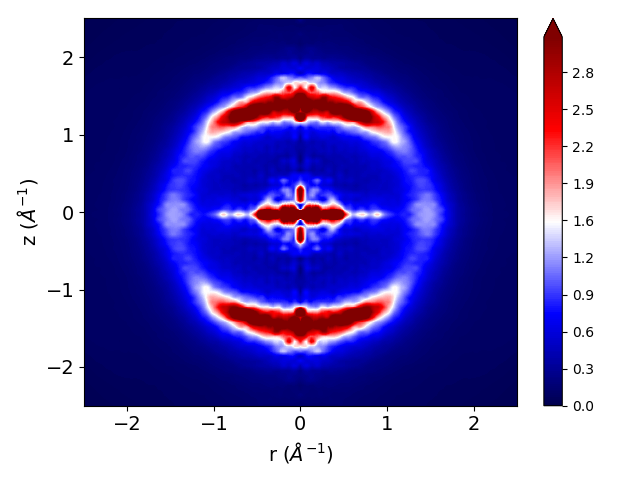
\includegraphics[width=\textwidth]{rzplot_layered_8.png}
%                \caption{8 mon/layer, Sandwiched}\label{fig:rzplot_layered_8}
%        \end{subfigure}
%        \begin{subfigure}{0.40\textwidth}
%                \centering
%                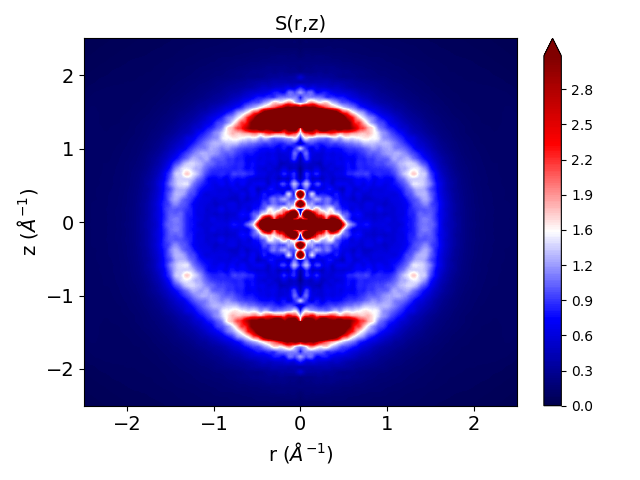
\includegraphics[width=\textwidth]{rzplot_offset_8.png}
%                \caption{8 mon/layer, Parallel Displaced}\label{fig:rzplot_offset_8}
%        \end{subfigure}
%	\caption{Simulated XRD patterns for all other configurations built with
%		 layers stacked 3.7 \AA~apart}\label{fig:XRDsim}
%  \end{figure}

%  \begin{wrapfigure}{R}{0.4\textwidth}
%      \centering
%      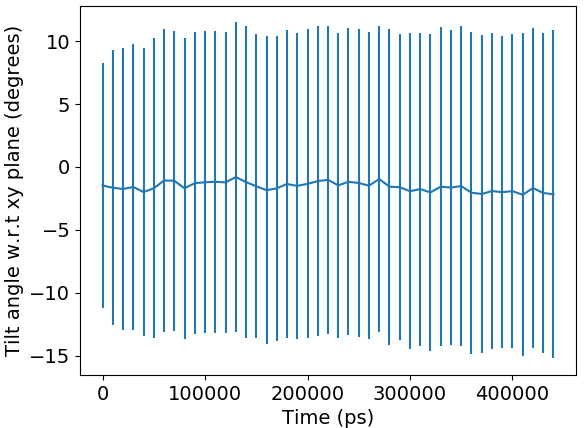
\includegraphics[width=0.4\textwidth]{tilt.png}
%      \caption{The average angle between alkane chains and the xy plane is nearly zero degrees}\label{fig:tilt}     
%  \end{wrapfigure}


%  \begin{figure}
%	\centering
%	\begin{subfigure}{0.45\textwidth}
%		\centering
%		\includegraphics[width=\textwidth]{ps5layered.png}
%		\caption{}\label(fig:ps5layered}
%	\end{subfigure}
%	\begin{subfigure}
%		\centering
%		\includegraphics[width=\textwidth]{ps5offset.png}
%		\caption{}\label{fig:ps5offset} 
%	\end{subfigure}
%  \end{figure}  
  
  \section{Ionic Conductivity}\label{section:ionic_conductivity}
 %BJC: add plot of collective diffusion values 
  In the main text, we calculated ionic conductivity using the Nernst-Einstein
  relationship. We also measured ionic conductivity using a second method, termed
  the collective diffusion model\cite{liu_collective_2013}, for robustness
  (Figure~\ref{fig:conductivity}). The collective diffusion model measures the
  movement of the collective variable, Q, which is defined as the amount of
  charge transfer through the system and can be thought to represent the center
  of charge of the system. The conductance, $\gamma$, of the system can be
  calculated as:
  \begin{equation}
	 \gamma = \dfrac{D_Q}{k_b T} 
	\label{eqn:collective_diffusion}
  \end{equation}
  $D_Q$ is the diffusion coefficient of the collective variable Q and is 
  calculated using the Einstein relation. We convert the resulting value
  to ionic conductivity by multiplying by channel length and dividing by
  the membrane cross sectional area. One can access a detailed derivation of 
  the model elsewhere\cite{liu_collective_2013}.
  
  \begin{figure}[!htb]
        \centering
        \includegraphics[width=0.5\linewidth]{Ionic_conductivity.png}
        \caption{The Collective Diffusion model and the Nernst-Einstein relation yield
        agreeing values of ionic conductivity for both types of ordered basin systems 
        simulated. Both methods estimate the value of the ionic conductivity to be an 
        order of magnitude higher than the experimental value. There is more noise in
        the collective diffusion model because there is inherently less data that 
        can be used for its calculation. For that reason, we use only the Nernst-Einstein relationship in the main text.}
        \label{fig:conductivity}
  \end{figure}  
  
  \section{Cross-linking algorithm details}\label{section:xlink}

  Crosslinking of the the monomer Na-GA3C11 occurs via a UV initiated free
  radical polymerization (FRP) (Figure~\ref{fig:xlink_mech}). Head-to-tail addition
  takes place between terminal vinyl groups on each of the monomer tails. We
  only considered head-to-tail addition since it is the dominant propagation mode
  in the real system.   

  \begin{figure}[!htb]
  \centering
  \includegraphics[width=\textwidth]{Crosslink_mechanism.eps}
  \caption{Terminal vinyl groups present on each monomer tail react with free
	  radical initiators to create monomers with terminal vinyl radicals.  Vinyl
	  radicals react with the vinyl groups of other monomers in order to propagate
	  crosslinking.}\label{fig:xlink_mech}
  \end{figure}
  
  We based our cross-linking algorithm on the known reaction mechanism.
  FRPs require an initiator which bonds to the system, meaning new atoms are
  introduced into the system. For simplicity, we simulated the initiator as
  hydrogen and made it present in the simulation by including them as dummy atoms
  in all possible locations where an addition could occur. We carry out the
  cross-linking procedure iteratively. During each iteration, the algorithm
  selects eligible bonding carbon atoms based on a distance cut-off. The algorithm
  then updates the topology with new bonds and changes dummy hydrogen atoms to appropriate
  hydrogen atom types. We only considered head-to-tail addition
  due to its dominance in the real system \cite{young_introduction_2011}. We did
  not consider direction of attack because the resultant mixture is racemic.

  Our implementation requires long simulation times to achieve high cross-link 
  densities. A typical cross-linking procedure can take up to 24 hours. In
  order to collect equilibrated data, further NPT simulation is necessary. We
  typically run a cross-linked system for an additional 100 ns to allow the system
  to readjust. For those reasons we did not cross-link all systems tested.
  
  \clearpage
  \section{The nematic order parameter}\label{method:nematic_order}

  We calculated the nematic order parameter for our system in order to
  understand the degree of ordering among monomer head groups. Typically, the
  nematic order parameter is calculated for nematic liquid crystal systems which
  are characterized by unidirectional ordering of liquid crystal monomers. The
  preferred direction of monomers is defined by the unit director vector,
  $\mathbf{n}$. Assuming a single preferred direction of alignment, the nematic
  order parameter, $S$, is defined as:~\cite{chaikin_principles_1995}
  \begin{equation}
	 S = \frac{1}{2} \langle(3\cos^2\theta -1)\rangle
	\label{eqn:nematic_order_parameter}
  \end{equation}
  where $\theta$ is the angle between the molecular long axis and $\mathbf{n}$.
  In a perfectly ordered nematic liquid crystal system, the molecular axis of each
  monomer should be aligned with $\mathbf{n}$ and give an order parameter of $S=1$. 
  We are interested in quantifying the degree of monomer head group alignment 
  between systems. We use Equation~\ref{eqn:nematic_order_parameter} to accomplish this
  by defining $\mathbf{n}$ as the $z$-axis (or pore axis), and then measuring the angles,
  $\theta$, between $\mathbf{n}$ and the vectors perpendicular to the plane of
  the aromatic head groups ($\mathbf{v}$ in Figure~\ref{fig:director}). 
  
  %BJC: change n to v in picture.
  \begin{figure}[!htb]
  \centering
  \includegraphics[width=0.75\linewidth]{nematic_director.png}
  \caption{We calculate the nematic order parameter by measuring the angle
  between $\mathbf{v}$ and the $z$-axis.}~\label{fig:director}
  \end{figure}

  The nematic order parameter is highest in sandwiched systems. 
  Figure~\ref{fig:nematic_distribution} shows the distribution of angles between
  the nematic director and the vector perpendicular to the monomer head groups. 
  Systems in the ordered basin have higher nematic order parameters than their
  disordered basin counterparts. Both sandwiched systems have higher nematic order
  parameters than both parallel displaced systems. This may occur because monomers
  in the sandwiched configuration have their motion restricted by vertically adjacent
  monomers, while those in the parallel displaced configuration have more room to 
  rotate.
  
  \clearpage

  \begin{figure}[!htb]
  \begin{subfigure}{\linewidth}
        \centering
        \begin{subfigure}{0.45\linewidth}
                \centering
                \includegraphics[width=\linewidth]{layered_nematic_order.png}
                \caption{Sandwiched, Ordered}~\label{fig:sandwich_nematic}
        \end{subfigure}%
        \begin{subfigure}{0.45\linewidth}
                \centering
                \includegraphics[width=\linewidth]{offset_nematic_order.png}
                \caption{Parallel Displaced, Ordered}~\label{fig:offset_nematic}
        \end{subfigure}
        \begin{subfigure}{0.45\linewidth}
                \centering
                \includegraphics[width=\linewidth]{disorder_sandwich_nematic_order.png}
                \caption{Sandwiched, Disordered}~\label{fig:disorder_sandwich_nematic}
        \end{subfigure}%
        \begin{subfigure}{0.45\linewidth}
                \centering
                \includegraphics[width=\linewidth]{disorder_offset_nematic_order.png}
                \caption{Parallel Displaced, Disordered}~\label{fig:disorder_offset_nematic}
        \end{subfigure}
  \end{subfigure}
  \caption{The distribution of angles between nematic director vector (see
	  Figure~\ref{fig:director}) and the $z$-axis averaged over the equilibrated portion
	  of each trajectory. The ordered sandwiched configuration has a higher nematic order
	  parameter than the ordered parallel displaced configuration. The disordered
	  sandwiched configuration has a higher nematic order parameter than the 
	  disordered parallel displaced configuration.}~\label{fig:nematic_distribution}
  \end{figure}

%BJC: now in main text
%  \section{Measurement of intensities of experimental and simulated XRD patterns}\label{section:xrd_intensities}
%  
%  We developed standardized methods of measuring the intensity of reflections of interest
%  in the experimental and simulated X-ray diffraction patterns presented in this work. Here,
%  we graphically illustrate the methods used for measuring these intensities. 
%  
%  All diffraction patterns are normalized according to R-alkanes and the intensities
%  of all reflections are reported relative to the intensity of R-alkanes. The region
%  used to calculate the average intensity of R-alkanes is shown in 
%  Figure~\ref{fig:ralkanes}. The top region is excluded because, in the simulated
%  patterns, R-$\pi$ intersects with R-alkanes.
%  
%  R-$\pi$ and R-double are reported as the maximum values of the peaks of the 
%  $q_z$ cross-section of the experimental pattern at $q_r=0$ (Figure~\ref{fig:rpi_rdouble}).
%  In the case of the experimental pattern, the peak heights are not symmetrical,
%  so we report the average of the two heights.
%  
%  We measured R-spots by calculating the average intensity within a region 
%  selected by visual inspection. We report the average intensity within the regions 
%  highlighted in red in Figure~\ref{fig:rspots}. If there are no easily discernible
%  spots, we report the average intensity at the intersection of R-alkanes with
%  the $q_z$ value of R-double since that is where we expect it to appear based on
%  experiment. Since R-double does not appear in our simulated patterns, we 
%  estimate where it should appear as half of the $q_z$ value of R-$\pi$.
%  
%  \begin{figure}[!htb]
%  \centering
%  \begin{subfigure}{0.45\linewidth}
%  \centering
%  \includegraphics[width=\textwidth]{WAXS_raw.png}
%  \caption{Unaltered experimental WAXS pattern}\label{fig:unaltered}
%  \end{subfigure}
%  \begin{subfigure}{0.45\linewidth}
%  \centering
%  \includegraphics[width=\textwidth]{ralkanes.png}
%  \caption{R-alkanes}\label{fig:ralkanes}
%  \end{subfigure}
%  \begin{subfigure}{0.45\linewidth}
%  \centering
%  \includegraphics[width=\textwidth]{rpi_rdouble.png}
%  \caption{$q_z|_{r=0}$}\label{fig:rpi_rdouble}
%  \end{subfigure}
%  \begin{subfigure}{0.45\linewidth}
%  \centering
%  \includegraphics[width=\textwidth]{rspots.png}
%  \caption{R-spots}\label{fig:rspots}
%  \end{subfigure}
%  \caption{}\label{fig:xrd_intensities}
%  \end{figure}
 
  \clearpage
 
  \section{Noise in simulated diffraction patterns}\label{section:xrd_noise}
  
  The magnitude of noise in the simulated diffraction patterns decreases as 
  the number of independent configurations increases (Figure~\ref{fig:xrd_noise}).
  We simulated the structure factor of 100 randomly placed particles and varied 
  the number of independent configurations (N). It is expected that the structure
  factor should resemble a two-dimensional Gaussian. We cannot sample enough 
  independent configurations of our system to completely eliminate noise.
  
  \begin{figure}[!htb]
  \centering
  \begin{subfigure}{0.45\linewidth}
  \centering
  \includegraphics[width=\textwidth]{xrd_1frame.png}
  \caption{N=1}
  \end{subfigure}
  \begin{subfigure}{0.45\linewidth}
  \centering
  \includegraphics[width=\textwidth]{xrd_10frame.png}
  \caption{N=10}
  \end{subfigure}
  \begin{subfigure}{0.45\linewidth}
  \centering
  \includegraphics[width=\textwidth]{xrd_100frame.png}
  \caption{N=100}
  \end{subfigure}
  \begin{subfigure}{0.45\linewidth}
  \centering
  \includegraphics[width=\textwidth]{xrd_10000frame.png}
  \caption{N=10000}
  \end{subfigure}
  \caption{The magnitude of noise, especially along $q_r$=0, decreases
  as the number of independent configurations (N) increases.}\label{fig:xrd_noise}
  \end{figure}
  
  \clearpage
%  \section{Experimental correlation length of R-$\pi$}\label{section:correlation_length}
% 
%  \vspace{1em}
%  Previous experimental studies of these systems did not calculate the correlation length, so we estimated it
%  from the raw 2D WAXS data. We took a slice of the 2D WAXS data along the dashed line in
%  Figure ~\ref{fig:waxs_dashed}. We removed background noise by subtracting the
%  intensity far from the pattern (high $q$) uniformly. We used a least squares
%  algorithm to fit a Lorentzian curve to the data. Only values recorded above
%  $q_z$ = 1.6 were considered for the fit in order to mitigate interference from
%  R-alkanes (Figure~\ref{fig:correlation_length_exp}). The full width at half
%  maximum (FWHM) is related to the correlation length, L, by the relationship: $
%  L = \frac{1}{FWHM} $. The error in the value is calculated as the square root
%  of the diagonal entry of the covariance matrix of optimized fit parameters.
%  We estimate the value of the correlation length to be 10 $\pm$ 1 using this 
%  method. Since the experimental peak width is also influenced by strain and 
%  instrumental broadening in addition to finite size broadening, the value 
%  calculated here is really only an upper bound on the correlation length. 
%  % need citations and more on Lorentzian parameters
%  \begin{figure}[!htb]
%  \centering
%  \begin{subfigure}{0.45\textwidth}	
%  	\includegraphics[width=\textwidth]{waxs_dashed.png}
%	\caption{}~\label{fig:waxs_dashed}
%  \end{subfigure}
%  \begin{subfigure}{0.45\textwidth}
%	\includegraphics[width=\textwidth]{Correlation_length_exp.png}
%	\caption{}~\label{fig:correlation_length_exp}
%  \end{subfigure}
%  \caption{(a) We estimated the system's experimental correlation length using a 
%  1D slice of the 2D WAXS patterns along $q_r$=0. (b) We fit a Lorentzian curve 
%  to the 1D slice. One of the fit parameters is the full width at half maximum (FWHM).
%  The correlation length is 1/FWHM.}~\label{fig:correlation}
%  \end{figure}
%  \vspace{1em} \\

  \section{The effect of imposed tail tilt}\label{section:tail_tilt}
  
  Monomer tails prefer to lie flat rather than tilt with respect to the
  membrane plane. We created a monomer whose tails tilt ca. 30$\degree$ with
  respect to the $xy$ membrane plane.  We added position restraints to the ends
  of the monomer tails with the same force constant as the head groups (see
  section~\ref{section:equilibration}).  As we slowly reduce the force constants,
  the tails begin to tend towards a negligible tilt angle
  (Figure~\ref{fig:tail_tilt}).
  
  \begin{figure}[!htb]
  \centering
  %MRSF2: seems to be missing in the repository? tilt_cat.png
  \includegraphics[width=0.5\textwidth]{tilt_cat.png}
  \caption{As we reduce the force constants applied to the end of each
  tail of an initially tilted monomer configuration, the average tilt 
  angle with respect to the membrane plane decreases until it is nearly
  negligible.}\label{fig:tail_tilt}
  \end{figure}

  \section{Tail organization}\label{section:tail_packing}
  
  In order to understand the origin of R-spots, we looked for ordering among
  the tails. We divided the tail into three sections: tail-fronts, tail-middles
  and tail-ends. The sections are illustrated in Figure~\ref{fig:tail_sections}.
  
  \begin{figure}[!htb]
  \centering
  \includegraphics[width=0.5\textwidth]{tail_sections.png}
  \caption{We divided the tail into three regions: tail-fronts (blue), 
  tail-middles (green) and tail-ends (red).}\label{fig:tail_sections}
  \end{figure}
  
  We plotted the center of masses of each tail section and measured the angle 
  between each center of mass and its nearest neighbor center of masses of the
  same tail section. For example, Figure~\ref{fig:centroids} shows a 3D plot of
  the center of masses of each tail front. We wanted to know the average location
  of nearest neighbors to each center of mass. The red bead in 
  Figure~\ref{fig:centroids} is a randomly selected center of mass. The
  green beads are the nearest neighbor center of masses to the red bead. We
  measured the angle between the red bead and each green bead with respect to
  the $xy$ plane. We repeated the same calculation for each center of mass at
  each simulation frame and were able to plot the average distribution shown
  in Figure~\ref{fig:tail_fronts}. We repeated the calculation for the tail
  middles (Figure~\ref{fig:tail_middles}) and the tail ends 
  (Figure~\ref{fig:tail_ends}). The amount of order decreases as we explore
  packing of tails farther from the head group.

  \begin{figure}[!htb]
        \centering
        \begin{subfigure}{0.45\textwidth}
        \includegraphics[width=\textwidth]{centroids.png}
		\caption{}\label{fig:centroids}
        \end{subfigure}
        \begin{subfigure}{0.45\textwidth}
        \includegraphics[width=\textwidth]{hexagonal_tail_packing.png}
        \caption{}\label{fig:tail_fronts}
        \end{subfigure}
        \begin{subfigure}{0.45\textwidth}
        \includegraphics[width=\textwidth]{hexagonal_tail_packing_middles.png}
        \caption{}\label{fig:tail_middles}
        \end{subfigure}
        \begin{subfigure}{0.45\textwidth}
        \includegraphics[width=\textwidth]{hexagonal_tail_packing_ends.png}
        \caption{}\label{fig:tail_ends}
        \end{subfigure}
        \caption{Monomer tails pack together hexagonally. (a) The center of mass
        of each tail-front (See Figure~\ref{fig:tail_sections}) is visualized as
        a blue sphere. The red sphere highlights an example of a tail-front 
        center of mass with its nearest neighbors (green spheres) surrounding it
        in a hexagonal pattern. (b) We calculated the angle between each tail-front
        center of mass and its nearest neighbor tail-front center of masses and 
        plotted the distribution. There are distinct peaks ca. $-60\degree$, $0\degree$ and
        $60\degree$ which is indicitive of hexagonal packing. (c) We repeated the 
        same procedure outlined in (a) and (b) with the tail-middles. There is still 
        a high degree of order. (d) We repeated the procedure again with the tail-ends.
        There is far less order at the ends of the tails where there is more
        space to fill.}\label{fig:tail_packing}
  \end{figure}
  
  \clearpage
  
  \section{Ensemble of ordered sandwiched configurations}\label{section:sandwiched_ensemble}
  
  Here we show the results of the same analysis shown in Figures~\ref{M-fig:ensemble_XRD} 
  and~\ref{M-fig:full_ensemble_distributions} of the main text for the 
  ordered sandwiched ensemble of configurations.
  
  \begin{figure}[!htb]
  \centering
  \begin{subfigure}{\textwidth}
  \includegraphics[width=\textwidth]{sandwiched_ensemble_pooled.pdf}
  \caption{Distributions of deviations from ideal positions generated with data
  from all independent simulations}\label{fig:offset_ensemble_pooled}
  \end{subfigure}
  \begin{subfigure}{\textwidth}
  \includegraphics[width=\textwidth]{sandwiched_ecdfs.pdf}
  \caption{Empirical cumulative distribution functions generated from (a) and
  from simulation ensembles.}\label{fig:offset_ecdfs}
  \end{subfigure}
  \caption{(a) The distributions of the head group COM deviations
  from their idealized positions generated using pooled data from all
  frames of each independent configuration are symmetric, implying that 
  there is equal probability for a head group to displace in the positive
  or negative $z$, $r$ or $\theta$-direction. (b) The COM position of a 
  given head group is displaced randomly upon quenching. The ECDF generated from
  the pooled distributions (black) in (a) agree with the means of the 
  ECDFs generated from each COM (red). The red error bars are larger than
  the black error bars since there is a wider distribution of mean COM
  deviations than the mean deviations of distributions sampled from the full
  distribution.}\label{fig:full_ensemble_distributions}
  \end{figure} 

  %MRSF: isn't this picture the same in the main draft of the document. Probably wouldn't have occured.
  %BJC: it's not identical. The main text uses the parallel displaced data.
  \begin{figure}[!htb]
  \centering
  \begin{subfigure}{0.49\textwidth}
  \includegraphics[width=\textwidth]{sandwiched_ensemble_stds.pdf}
  \caption{}\label{fig:offset_ensemble_stds}
  \end{subfigure}
  \begin{subfigure}{0.49\textwidth}
  \includegraphics[width=\textwidth]{sandwiched_ensemble_means.pdf}
  \caption{}\label{fig:offset_ensemble_means}
  \end{subfigure}
  \begin{subfigure}{\textwidth}
  \includegraphics[width=\textwidth]{sandwiched_ensemble_regional_density.pdf}
  \caption{}\label{fig:offset_ensemble_regional_density}
  \end{subfigure}
  \caption{(a) The standard deviation of the distribution of quenched disorder
  from the first 5 ns of the main ordered sandwiched system studied in
  this paper (black dashed line) is in agreement with the distribution of quenched disorder 
  standard deviations calculated from the ensemble of simulations (histogram). 
  (b) The mean values of $r$ and $\theta$ from the first 5 ns of the main
  system trajectory (black dashed line) is in agreement with the distribution of mean values
  calculated from each simulation in the ensemble (histogram). The mean values of $z$
  are necessarily 0 so they are not plotted. (c) The radial densities of tail
  atoms, head group atoms and sodium atoms calculated from the first 5 ns of the
  main system simulation trajectory (black lines) and from the ensemble of 
  trajectories (all other lines) look qualitatively similar.}\label{fig:ensemble_stds}
  \end{figure}
  
  \clearpage

  \section{Carboxylate Dihedrals}

  It is most energetically favorable for the carboxylate group attached to the monomer
  head groups to stay coplanar with the phenyl group to which it is attached
  (Figure~\ref{fig:carboxylate_dihedral_rb}). Although GAFF may over-predict the penalty
  for deviating from its minimum energy configuration relative to those calculated 
  by Rakitin and Pack~\cite{rakitin_necessity_2005} and Nelson and
  Borkman~\cite{nelson_internal_1998}, they all show that there is an appreciable barrier
  to rotation about the carboxylate-phenyl bond. The potential energy reaches its maximum
  at rotation angles corresponding to a carboxylate group that is antiparallel to the 
  plane of the phenyl ring to which it is attached (90\degree and 270\degree).
  
  \begin{figure}[!htb]
  \centering
  %MRSF2: figure missing in repository. 
  \includegraphics[width=0.5\textwidth]{carboxylate_dihedrals.pdf}
  \caption{A potential energy diagram for the dihedral angle about the carbon-carbon bond of
  a carboxylate group attached to an aromatic ring, using parameters from GAFF (blue), 
  Rakitin (orange) and Borkman (green). It is energetically favorable for the 
  carboxylate group to stay in plane with the aromatic ring. There is a large energy 
  penalty as the dihedral becomes antiparallel to the plane of the aromatic 
  ring.}\label{fig:carboxylate_dihedral_rb}
  \end{figure}

  \clearpage
% BJC: not necessary
%  \begin{figure}[!htb]
%  \centering
%        \begin{subfigure}{0.45\textwidth}
%                \includegraphics[width=\textwidth]{water_filled_pore.png}
%                \caption{}\label{fig:water_filled_pores}
%        \end{subfigure}
%        \begin{subfigure}{0.45\textwidth}
%                \includegraphics[width=\textwidth]{water_removed.png}
%                \caption{}\label{fig:water_removed}
%        \end{subfigure}
%  \caption{(a) Pores built in the parallel displaced configuration with 5
%	  monomers per layer are filled with 5 wt\% water. (b) The same system is
%	  visualized with water molecules and sodium ions removed. Head groups vacate the
%	  pore region leaving an aqueous solution of water and sodium ions.}\label{fig:water_pores}
%  \end{figure}

% BJC: a lot of this is in the main text, but there is some other potentially usefull stuff in here
%  \section{Demonstrative Fourier transforms}\label{section:fourier}
%  
%  Here we use Fourier transforms to demonstrate some of the arguments made in 
%  the main text. Interpretation of real and simulated X-ray diffraction patterns
%  is non-trivial and requires careful thought. They are a function of the positions
%  of all atoms in space, and suffer from the phase problem. Namely, there are multiple
%  solutions that could explain a single diffraction pattern. Using simplified models, 
%  we can hypothesize about the effect of various configurations on the simulated patterns.
%
%  \subsection{Magnitude of R-$\pi$}\label{section:rpi_ft}
%  
%  In all cases, the magnitude of R-$\pi$ in our system is larger than that in experiment.
%  Some of the discrepancy can be explained by defects and imperfect pore alignment. 
%  However, there are significant effects resulting from the ordered states that we simulate.
%  
%  Persistent oscillations in the z-correlation function, $g(z)$, increase the intensity of R-$\pi$. 
%  In Figure~\ref{fig:z_correlation}, we fit a decaying sinusoidal function 
%  (equation~\ref{M-eqn:decaying_sinusoid} of the main text) to $g(z)$ calculated from the
%  sandwiched configuration in the ordered basin. While the sinusoidal decay fit decays to one
%  rather quickly, $g(z)$ continues to oscillate with nearly the same amplitude as its third peak. 
%  In Figure~\ref{fig:theoretical_correlation_functions}, we overlay the same decaying sinusoidal
%  fit with a function that continues to oscillate with the same amplitude as the third peak of
%  the fit to $g(z)$. In Figure~\ref{fig:power_spectrum_comparison}, we plot the power spectrum
%  generated from the discrete Fourier transform of the plots in Figure~\ref{fig:theoretical_correlation_functions}. 
%  The maximum intensity of the power spectrum increases by nearly 60\% when the correlation 
%  function does not decay to one. This explains, in part, the large simulated value of the
%  intensity of R-$\pi$.
%  
%  \begin{figure}[!htb]
%  \centering
%  \begin{subfigure}{0.32\textwidth}
%  \includegraphics[width=\textwidth]{z_correlation_layered_sinefit.png}
%  \caption{}\label{fig:z_correlation}
%  \end{subfigure}
%  \begin{subfigure}{0.32\textwidth}
%  \includegraphics[width=\textwidth]{theoretical_correlation_functions.png}
%  \caption{}\label{fig:theoretical_correlation_functions}
%  \end{subfigure}
%  \begin{subfigure}{0.32\textwidth}
%  \includegraphics[width=\textwidth]{power_spectrum_comparison.png}
%  \caption{}\label{fig:power_spectrum_comparison}
%  \end{subfigure}
%  \caption{(a) We fit a decaying sinusoidal function to the z-correlation function, $g(z)$, 
%  calculated from the ordered basin sandwiched system. The oscillations in $g(z)$ continue
%  to oscillate at nearly the same amplitude as its third peak. (b) We overlaid a plot of the
%  fit to $g(z)$ with a similar function that continues to oscillate with the same amplitude
%  as its third peak. (c) The power spectrum of each plot in (b) exhibits a 60\% increase in
%  intensity of the peaks when the function does not decay to 1.}\label{fig:rpi_ft}
%  \end{figure}
%  
%  \subsection{Simplified assemblies}\label{section:simplified_assemblies}
%  
%  We explored the sandwiched and parallel displaced configurations as potential ways for
%  aromatic head groups to stack. We used copies of the same monomer to build each system.
%  We were unable to create any assemblies which exhibited R-double using this technique. 
%  We simulated diffraction patterns of simplified configurations to understand why. We 
%  placed points in array that resemble the sandwiched and parallel displaced configurations.
%  Points are space 3.7 $\AA$ apart so it is easy to relate them to LLC membrane system.
%  5 columns of points are placed 5 $\AA$ from a defined "pore center".
%  
%  When points are stacked in either configuration, R-double cannot appear. In the case
%  of the sandwiched configuration, the fundamental frequency is set at 1.7 $\AA^{-1}$,
%  the same location as R-$\pi$. Subharmonics appear at integer multiples of this frequency.
%  The parallel displaced configuration exhibits reflections at half the $q_z$ value of
%  R-$\pi$, which is where we expect to see R-double. However, just like the LLC membrane
%  system, the reflections appear away from $q_r=0$ and are caused by the helical stacking
%  arrangement. 
%  
%  From these observations, it is clear that, in order to make R-double appear in our simulated
%  diffraction patterns, we must create systems with asymmetries along the z-axis which lead to
%  a fundamental frequency of $0.85 \AA^{-1}$. This requires a modulation in electron density 
%  every 7.4 $\AA$. This line of thought gave rise to the systems studied in 
%  section~\ref{M-section:rdouble} of the main text.
%  
%  \begin{figure}[!htb]
%  \centering
%  \begin{subfigure}{0.45\textwidth}
%  \includegraphics[width=\textwidth]{simple_sandwich_realspace.png}
%  \caption{}\label{fig:simple_sandwich_realspace}
%  \end{subfigure}
%  \begin{subfigure}{0.45\textwidth}
%  \includegraphics[width=\textwidth]{simple_sandwich_rzplot.png}
%  \caption{}\label{fig:simple_sandwich_rzplot}
%  \end{subfigure}
%  \begin{subfigure}{0.45\textwidth}
%  \includegraphics[width=\textwidth]{simple_offset_realspace.png}
%  \caption{}\label{fig:simple_offset_realspace}
%  \end{subfigure}
%  \begin{subfigure}{0.45\textwidth}
%  \includegraphics[width=\textwidth]{simple_offset_rzplot.png}
%  \caption{}\label{fig:simple_offset_rzplot}
%  \end{subfigure}
%  \caption{}\label{fig:simple_FTs}
%  \end{figure}
  
  \section{All solvated systems}\label{section:solvation}
  
  % formatting taken from : https://tex.stackexchange.com/questions/239715/add-titles-for-rows-and-columns-in-a-subfloat
  \newlength{\tempdima}
  \newcommand{\rowname}[1]% #1 = text
  {\rotatebox{90}{\makebox[\tempdima][c]{\textbf{#1}}}}
  
  \renewcommand{\thesubfigure}{\alph{subfigure}}
  \newcommand{\mycaption}[1]% #1 = caption
  {\refstepcounter{subfigure}\textbf{(\thesubfigure) }{\ignorespaces #1}}  
  
  \begin{figure}[!htb]
  \begin{subfigure}{0.915\textwidth}
  	\settoheight{\tempdima}{\includegraphics[width=.32\linewidth]{solvated_offset_rzplot_1.png}}%
  	\centering\begin{tabular}{@{}c@{ }c@{ }c@{ }c@{}}
  	&\textbf{1 wt\%} & \textbf{\hspace{2em}2.5 wt\%} & \textbf{5 wt\%} \\
  	\rowname{Parallel Displaced}&
  	\includegraphics[width=.28\linewidth,trim={1cm 0 1.3cm 0},clip]{solvated_offset_rzplot_1.png}&
  	\includegraphics[width=.28\linewidth,trim={1cm 0 1.3cm 0},clip]{solvated_offset_rzplot_25.png}&
  	\includegraphics[width=.28\linewidth,trim={1cm 0 1.3cm 0},clip]{solvated_offset_rzplot_5.png}\\[-1ex]
  	%&\mycaption{0.2} & \mycaption{0.2} & \mycaption{0.3}\\
  	\rowname{Sandwiched}&
  	\includegraphics[width=.28\linewidth,trim={1cm 0 1.3cm 0},clip]{solvated_layered_rzplot_1.png}&
  	\includegraphics[width=.28\linewidth,trim={1cm 0 1.3cm 0},clip]{solvated_layered_rzplot_25.png}&
  	\includegraphics[width=.28\linewidth,trim={1cm 0 1.3cm 0},clip]{solvated_layered_rzplot_5.png}\\[-1ex]
  	%\mycaption{0.5} & \mycaption{0.6} & \mycaption{0.7} \\
  	\end{tabular}
  \end{subfigure}
  \begin{subfigure}{0.075\textwidth}
  	\includegraphics[width=\textwidth]{colorbar_jet.png}
  \end{subfigure}
	\caption{Adding 1 wt\% water to the ordered basin dry systems causes an increase in the intensity
	R-spots. R-double becomes visible in the parallel displaced configuration. Additional amounts
	of water increase discrepancies with experiment} %MRS7:by increasing disorder?
  \label{fig:solvation}

  \end{figure}
  
  \clearpage
  \section{The role of water in the appearance of R-double}\label{section:rdouble}
  
  The appearance of R-double is likely a consequence of structure induced when
  vertically stacked monomer pairs share hydrogen bonds with a common water molecule (See
  Section~\ref{M-section:rdouble} of the main text). We quantified the occurence of
  these pairing interactions by binning the $z$-positions of the center of mass of 
  the monomer head groups into 20 bins, the same number as the monomers per column. 
  This works relatively well since there is a high degree of correlation between
  columns in our system. Peaks in the distributions represent the scenario where a monomer head group
  shares a water molecule with a head group vertically above it (See Figure~\ref{fig:pore_hbonds}).
  We calculated the discrete Fourier transform of the distributions in Figure~\ref{fig:pore_hbonds}
  which we used as a rough indicator of whether the head group arrangement will lead to R-double
  (Figure~\ref{fig:pore_hbonds_ft}). We see the strongest indicator of asymmetric monomer
  stacking in Pore 1 where the peaks at 0.76 $\AA^{-1}$ are clearly distinguishable, meaning
  there is periodicity at twice the $\pi$-stacking distance.
  
  \begin{figure}[!htb]
  \centering
  \begin{subfigure}{0.45\textwidth}
  \includegraphics[width=\textwidth]{pore_hbonds.png}
  \caption{}\label{fig:pore_hbonds}
  \end{subfigure}
  \begin{subfigure}{0.45\textwidth}
  \includegraphics[width=\textwidth]{pore_hbonds_ft.png}
  \caption{}\label{fig:pore_hbonds_ft}
  \end{subfigure}
  \caption{(a) We group the $z$-coordinate of the center of mass of monomer
  head groups into 20 bins. Peaks in the distributions indicate a shared hydrogen bonded
  water molecule between a monomer head group and one in the bin vertically above it. 
  The distance between the peaks roughly corresponds to the distance between pairs of 
  monomers. The distance between peaks in pore 1 (indicated by arrows) is equal to two 
  times the $\pi$-stacking distance. In this scenario, monomers are no longer evenly spaced
  in the $z$-direction since they are pulled closer together by hydrogen bonds. (b) We 
  performed discrete Fourier transforms on each distribution in (a) In Pore 1, there 
  is periodicity every 8.3 $\AA$, twice the $\pi$-stacking distance, as indicated by the
  intensity at 0.76 $\AA^{-1}$. In this case, the center of mass of two adjacent pairs 
  is separated by twice the average monomer stacking distance, while the four monomers 
  involved are unequally spaced. These conditions seem likely to give rise to R-double.
  }\label{fig:hbonds}
  \end{figure}
  
  \section{Diffusion of monomers}

  We calculated the diffusion coefficient of the monomer head groups by measuring
  the slope of the linear region of their mean squared displacement curves accumulated
  over the length of the equilibration simulations (Table~\ref{table:msd}). 
  
  \begin{table}[h]
  \centering
  \begin{tabular}{cc}
  \toprule
  System & Diffusion Constant ($m^2/s$) \\ 
  \midrule
  Sandwiched, Ordered & $1.4 \times 10^{-14}$ \\
  Parallel Displaced, Ordered & $2.0 \times 10^{-14}$ \\
  Sandwiched, Disordered & $2.0 \times 10^{-14}$ \\
  Parallel Displaced, Disordered & $3.5 \times 10^{-14}$ \\
  Parallel Displaced, 1 wt \% water & $7.1 \times 10^{-14}$ \\
  \bottomrule
  \end{tabular}
  \caption{The diffusion constants for all systems are on the order of $10^{-14} m^2/s$ 
  .}~\label{table:msd}
  \end{table}
  
  \section{Autocorrelation of monomer dihedrals}
  
  In section~\ref{M-section:slow_dynamics} of the main text, we calculated the
  autocorrelation function of the outer tail either dihedrals pictured
  in Figure~\ref{fig:dihedrals}.
  
  \begin{figure}[!htb]
  \centering
  \includegraphics[width=0.5\textwidth]{monomer_dihedrals.png}
  \caption{We measured the autocorrelation functions of the dihedrals highlighted in
  black. We only included dihedrals associated with the outer tails in our calculation
  since the position of the center tail leads to fundamentally different interactions and
  dynamics.}\label{fig:dihedrals}
  \end{figure}
  
%  \begin{figure}[!htb]
%  \centering
%  \begin{subfigure}{width=0.45\textwidth}
%  \includegraphics[width=\textwidth]{rdouble_offset_solvated_rzplot.png}
%  \caption{}\label{fig:rdouble_offset_solvated_rzplot}
%  \end{subfigure}
%  \begin{subfigure}{width=0.45\textwidth}
%  \includegraphics[width=\textwidth]{rzplot_pore1_removed.png}
%  \caption{}\label{fig:rzplot_pore1_removed}
%  \end{subfigure}
%  \caption{(a) The simulated diffraction pattern of a system simulated in an ordered basin 
%  parallel displaced configuration with 1 wt\% water shows R-double at $mathbf{q}=(0, 0.7) \AA^{-1}$.
%  (b) When we remove }\label{fig:pore1_removed}
%  \end{figure}

\clearpage
\bibliography{llc}
\end{document}

% LocalWords:  Na GA Packmol pdb filetype MarvinSketch noauthor nodate GROMACS
% LocalWords:  atomtypes antechamber inpcrd prmtop acpype py silva gro gmx NVT
% LocalWords:  editconf molcharge bccsym cyan png dihedrals pore's ca pt xy kJ
% LocalWords:  kinetically metastable outlier BJC Berendsen barostat Parrinello
% LocalWords:  Rahman solvated solvate Eq XRD alkanes WAXS exp FWHM mon alkane
% LocalWords:  transitioning topview rzplot traj binned wt LLC Subharmonics UV
% LocalWords:  realspace Crosslinking polymerization FRP crosslinking FRPs rb
% LocalWords:  racemic Nernst carboxylate antiparallel llc
